
% documentclass options:
% ngerman is needed for hyphenation if the thesis contains parts written in German
% BCOR is binding correction
% if you'd rather have a one sided thesis, add `onside' to the documentclass
\documentclass[11pt, a4paper, BCOR=10mm, english, ngerman]{scrbook}

% include all packages and define commands in setup.tex

%------------------------------------------------------------------------------
%       package includes
%------------------------------------------------------------------------------
    % font encoding is set up for pdflatex, for other environments see
    % http://tex.stackexchange.com/questions/44694/fontenc-vs-inputenc
    \usepackage[T1]{fontenc}  % 8-bit fonts, improves handling of hyphenations
    \usepackage{booktabs}
    \usepackage[utf8x]{inputenc}
    % provides `old' commands for table of contents. Eases the ability to switch
    % between book and scrbook
    \usepackage{scrhack}
    \usepackage{subcaption}
    \usepackage{adjustbox}
    \usepackage{multirow}
    \usepackage{threeparttable}

    %add packages for text color


    % ------------------- layout, default -------------------
    % adjust the style of float's captions, separated from text to improve readabilty
    \usepackage[labelfont=bf, labelsep=colon, format=hang, textfont=singlespacing]{caption}
    \usepackage{chngcntr}  % continuous numbering of figures/tables over chapters
    \counterwithout{equation}{chapter}
    \counterwithout{figure}{chapter}
    \counterwithout{table}{chapter}

    % Uncomment the following line if you switch from scrbook to book
    % and comment the setkomafont line
    %\usepackage{titlesec}  % remove "Chapter" from the chapter title
    %\titleformat{\chapter}[hang]{\bfseries\huge}{\thechapter}{2pc}{\huge}
    \setkomafont{chapter}{\normalfont\bfseries\huge}

    \usepackage{setspace}  % Line spacing
    \onehalfspacing
    % \doublespacing  % uncomment for double spacing, e.g. for annotations in correction

    % ------------------- functional, default-------------------
    \usepackage[dvipsnames]{xcolor}  % more colors
    \usepackage{array}  % custom format per column in table - needed on the title page
    \usepackage{graphicx}  % include graphics
    %\usepackage{subfig}  % divide figure, e.g. 1(a), 1(b)...
    \usepackage{amsmath}  % |
    \usepackage{amsthm}   % | math, bmatrix etc
    \usepackage{amsfonts} % |
    \usepackage{calc}  % calculate within LaTeX
    \usepackage[unicode=true,bookmarks=true,bookmarksnumbered=true,
                bookmarksopen=true,bookmarksopenlevel=1,breaklinks=false,
                pdfborder={0 0 0},backref=false,colorlinks=false]{hyperref}


    %==========================================
    % You might not need the following packages, I only included them as they
    % are needed for the example floats
    % ------------------- functional, custom -------------------
    \usepackage{algorithm,algpseudocode}
    \usepackage{bm}  % bold greek variables (boldmath)
    \usepackage{tikz}
    \usetikzlibrary{positioning}  % use: above left of, etc

    % Improves general appearance of the text
    \usepackage[protrusion=true,expansion=true, kerning]{microtype}

%------------------------------------------------------------------------------
%       (re)new commands / settings
%------------------------------------------------------------------------------
    % ----------------- referencing ----------------
    \newcommand{\secref}[1]{Section~\ref{#1}}
    \newcommand{\chapref}[1]{Chapter~\ref{#1}}
    \renewcommand{\eqref}[1]{Equation~(\ref{#1})}
    \newcommand{\figref}[1]{Figure~\ref{#1}}
    \newcommand{\tabref}[1]{Table~\ref{#1}}

    %changing line spacing to 1.5
    \renewcommand{\baselinestretch}{1.2}

    % ------------------- colors -------------------
    \definecolor{darkgreen}{rgb}{0.0, 0.5, 0.0}
    % Colors of the Albert Ludwigs University as in
    % https://www.zuv.uni-freiburg.de/service/cd/cd-manual/farbwelt
    \definecolor{UniBlue}{RGB}{0, 74, 153}
    \definecolor{UniRed}{RGB}{193, 0, 42}
    \definecolor{UniGrey}{RGB}{154, 155, 156}


    % ------------------- layout -------------------
    % prevents floating objects from being placed ahead of their section
    \let\mySection\section\renewcommand{\section}{\suppressfloats[t]\mySection}
    \let\mySubSection\subsection\renewcommand{\subsection}{\suppressfloats[t]\mySubSection}


    % ------------------- marker commands -------------------
    % ToDo command
    \newcommand{\todo}[1]{\textbf{\textcolor{red}{(TODO: #1)}}}
    \newcommand{\extend}[1]{\textbf{\textcolor{darkgreen}{(EXTEND: #1)}}}
    % Lighter color to note down quick drafts
    \newcommand{\draft}[1]{\textbf{\textcolor{NavyBlue}{(DRAFT: #1)}}}


    % ------------------- math formatting commands -------------------
    % define vectors to be bold instead of using an arrow
    \renewcommand{\vec}[1]{\mathbf{#1}}
    \newcommand{\mat}[1]{\mathbf{#1}}
    % tag equation with name
    \newcommand{\eqname}[1]{\tag*{#1}}

    %New command for frequently used terms%
    \newcommand{\gvit}{GroupViT }
    \newcommand{\ovs}{OVSegmentor }
    \newcommand{\pvoc}{PASCAL VOC }
    \newcommand{\pcon}{PASCAL Context }
    \newcommand{\coco}{MSCOCO }
    \newcommand{\ad}{ADE 20K }
    \newcommand{\mIoU}{Mean Intersection Over Union }


    % ------------------- pdf settings -------------------
    % ADAPT THIS
    \hypersetup{pdftitle={The great title!},
                pdfauthor={FirstName LastName},
                pdfsubject={Undergraduate thesis at the Albert Ludwig University of Freiburg},
                pdfkeywords={deep learning, awesome algorithm,  undergraduate thesis},
                pdfpagelayout=OneColumn, pdfnewwindow=true, pdfstartview=XYZ, plainpages=false}


    %==========================================
    % You might not need the following commands, I only included them as they
    % are needed for the example floats

    % ------------------- Tikz styles -------------------
    \tikzset{>=latex}  % arrow style


    % ------------------- algorithm ---------------------
    % Command to align comments in algorithm
    \newcommand{\alignedComment}[1]{\Comment{\parbox[t]{.35\linewidth}{#1}}}
    % define a foreach command in algorithms
    \algnewcommand\algorithmicforeach{\textbf{foreach}}
    \algdef{S}[FOR]{ForEach}[1]{\algorithmicforeach\ #1\ \algorithmicdo}

\usepackage[T1]{fontenc}
\usepackage{lmodern}


\begin{document}
    \pagestyle{empty} % no header and no page number
    % disable hyper links to remove warning "destination with same identifier"
    % this means within this section nothing can be referenced with a hyperlink
    \hypersetup{pageanchor=false}
    
\begin{titlepage}
\begin{center}

\newcommand{\HorizontalLine}{\rule{\linewidth}{0.3mm}}

{\Large Master's Thesis}\\[1.3cm]


% _____________________________________________________________________________
\HorizontalLine \\[0.4cm]
\begin{spacing}{2
}
    {\huge \bfseries Tackling the Challenges of Unsupervised Object Detection} \\
\end{spacing}
\HorizontalLine \\[1.5cm]
% _____________________________________________________________________________


{\Huge Ajesh Krishnan Kizhakke Menakath} \\[2cm]


\begin{tabular}[hc]{>{\huge}l >{\huge}l}
  
  Advisers: & Silvio Galesso \\[1.2cm]
  Examiner: & Prof. Dr. Thomas Brox \\[0.2cm]
    &          Prof. Dr. Matthias Teschner \\[0.3cm]
\end{tabular}
\vfill  % move the following text to the bottom

\Large {
    Albert-Ludwigs-University Freiburg\\
    Faculty of Engineering\\
    Department of Computer Science\\
    Chair of Pattern Recognition and Image Processing\\[1cm]

    August 23\textsuperscript{th}, 2024\\
}
\end{center}
\end{titlepage}

% title page back
\ \vfill \ \\  % at least one space required before vfill
\
\textbf{Writing period}            \smallskip{} \\
23.\,02.\,2023 -- 23.\,08.\,2023   \bigskip{} \\
\
\textbf{Examiner}                  \smallskip{} \\
Prof. Dr. Thomas Brox              \bigskip{} \\
\
\textbf{Second Examiner}                  \smallskip{} \\
Prof. Dr. Matthias Teschner           \bigskip{} \\
\
\textbf{Advisers}                  \smallskip{} \\
Silvio Galesso

    \pagestyle{plain} % remove chapter name from top, page number at the bottom
    \frontmatter  % roman page numbers
    % official declaration from the examination office; to be sure double
% check the wording on their website
% (https://www.tf.uni-freiburg.de/studies/exams/thesis/thesis_formatting.html#erklaerung)

\chapter*{Declaration}

I hereby declare, that I am the sole author and composer of my thesis and that no other sources or learning aids, other than those listed, have been used. Furthermore, I declare that I have acknowledged the work of others by providing detailed references of said work.  \newline
I hereby also declare, that my Thesis has not been prepared for another examination
or assignment, either wholly or excerpts thereof.
\\[3\normalbaselineskip]
\begin{tabular}{p{\textwidth/2} l}
  \rule{\textwidth/3}{0.4pt}   &   \rule{\textwidth/3}{0.4pt} \\
  Place, Date                  &   Signature
\end{tabular}
    \chapter*{Abstract}
This thesis focuses on advancing unsupervised object detection and instance segmentation by building upon and improving the CutLER framework. While CutLER has demonstrated significant potential in unsupervised learning tasks, it exhibits limitations, particularly in handling overlapping instances and dependence on initial masks. This work investigates these limitations in detail.

To address these challenges, we propose three key contributions. First, a detailed study of the effects of overlapping instances is conducted, which leads to the decision to remove images with overlapping instances from the training set. This adjustment resulted in observed improvements in model performance. Second, we verify the hypothesis that object-centricity of images contributes to better instance discrimination capabilities.  Finally, we introduce a refined mask filtration scheme that improves the quality of the pseudo-ground truth masks generated by the MaskCut method. By removing ambiguous and low-confidence masks during training, the proposed approach effectively reduces noise and enhances the precision of mask predictions.

Experiments conducted across diverse datasets, including COCO and PASCAL VOC, validate the effectiveness of the proposed improvements. The results consistently show performance gains in both detection and segmentation tasks, underscoring the importance of addressing overlapping instances and refining mask annotations in unsupervised learning. This thesis not only seeks to enhance the performance of the CutLER framework but also provides valuable insights into the challenges and opportunities inherent in unsupervised object detection and segmentation.
%In the evolving realm of deep learning for scene understanding, the traditional dichotomy between grouping and recognition has blurred, thanks to integrated end-to-end training systems. Yet, GroupViT reshapes this landscape by reintroducing explicit grouping in deep networks. This novel bottom-up approach rekindles the essence of semantic segmentation in contrasts with traditional top-down methods. GroupViT, trained on weak supervisory signals from text, showcases impressive results across various datasets, highlighting its efficacy for open-vocabulary segmentation. 
%% By identifying and grouping coherent concepts before labeling, GroupViT remarkably aligns segmentation performance with human perception. 
%
%
%Within this thesis, we undertake a dissection of the pretrained GroupViT model, isolating two pivotal components for open-vocabulary segmentation: Visual Grouping and Vision-Text Alignment. Based on our analysis, it becomes evident that there is substantial room for improvement, particularly in Visual Grouping. By leveraging GroupViT’s pretrained model and further training on a cleaner, smaller MSCOCO dataset, we observed promising enhancements on the dataset. However, there are trade-offs, compromising performance on downstream dataset such as PASCAL VOC and PASCAL Context.
%% By capitalizing on GroupViT's existing knowledge and training the relevant components on cleaner and smaaler MSCOCO dataset, promising enhancements emerge on the validation split. However, these gains come with trade-offs, as performance on downstream datasets is compromised.
%
%To address these challenges, this work introduces strategic enhancements. First, we incorporate entropy regularization techniques to improve semantic grouping and visual-text alignment. Second, we propose a non-noisy contrastive loss, countering limitations of training on a smaller dataset and leading to more robust, accurate results.
%% To tackle these challenges, the dissertation introduces strategic enhancements. One of these enhancements involves the incorporation of entropy regularization techniques. By implementing these techniques, the dissertation seeks to improve the process of grouping semantic concepts and aligning visual and textual elements more effectively. Another significant enhancement proposed is the adoption of a non-noisy contrastive loss. This approach addresses the inherent limitations associated with training on a smaller dataset, ultimately leading to more robust and accurate results.
%
%These systematic refinements furnish a framework to further train the pretrained model of  GroupViT on smaller and cleaner datasets for segmentation, while upholding the performance across datasets.
%% By methodically implementing these refinements, the dissertation provides a robust framework for fine-tuning a pretrained GroupViT model on a more streamlined datasets, preserving performance standards across downstream applications.
%% Deviating from Biological vision, Deep learning netwroks have blurred the distinction between between grouping and  recognition following the top-down approach. This Thesis explores and enhances GroupViT that approached semantic segmentation like HUmans, by finding and grouping coherent concepts and finaaly label them in a bottom-up manner. This results in fucntioning of segmentation closer to humar perception. GroupViT training on weak supervisory signals of text achieves remarkable performance on many downstream datasets making it suitable for open-vocabulary segmentation.
%
%
%%  In this Thesis, we examine the pretrained model of GroupViT by decoupling teo of its major components for the task of open-vocabulary segmentation called Visual Grouping and Vision-Text alignment and examining them indivisually. We found that although both of them have some room of improvement, Visual Grouping has a bigger one . While utilizing the pretrained knowledge of GroupViT , training relevant components on a cleaner, smaller dataset of MSCOCO, we observed improved performance on the validation split of training dataset but big comprise on downstream datasets. We proceeded with making targetted improvements (i) Firstly we proposes entropy regularization methods to improved grouping of cohesive concepts and improve visual-text alignment (ii) We propose non-noisy contrastive loss due to training on smaller datasets.
%
%%  This strategic and step-wise improvement provides an effective recipe to train a pretrained model of GroupViT on a cleaner smaller dataset without comprising its performance on downstream datasets
%
%% I am further investigating the potential of GroupVIT on cleaner, smaller but more challenging datasets such as COCO. GroupViT combines a hierarchical grouping architecture with VIT to achieve semantic segmentation using only text supervision. The grouping mechanism of GroupVIT learns to group similar image regions for segmentation by comparing segment-level embeddings to those derived from captions through contrastive learning. As part of our current roadmap, we plan to explore a new localized paired loss, which will aim to align grouped image segments with specific words or pairs of words in the text caption at different levels of grouping hierarchy. GroupVIT currently uses a multi-label contrastive loss that aims to align emerged grouped segments with entire captions. However, we believe that localizing the loss to the parts of the caption that represent the emerged grouped segments could improve the performance of GroupVIT by targetting localized semantic similarity. In addition, we will investigate different levels of hierarchy to explore the efficiency of the model.
    \tableofcontents
    \listoffigures
    \listoftables
    \hypersetup{pageanchor=true}  % re-enable hyperlinking

    \mainmatter  % Arabic page numbers
    \chapter{Introduction}\label{chap:introduction}

\section{Motivation}
Instance detection is a fundamental challenge in computer vision with critical applications in fields ranging from autonomous driving to medical imaging. Recent advancements have seen a shift from traditional Convolutional Neural Networks (CNNs) to the transformative capabilities of Transformers, as demonstrated by Dosovitskiy et al. (2020) with their Vision Transformer (ViT)~\cite{dosovitskiy2020image}. Subsequently, the concept of utilizing deep ViT features as dense visual descriptors was introduced by Amir et al. (2021)~\cite{amir2021deep}, highlighting the strong semantic information these descriptors provide about instances within an image. This shift highlights a growing interest in leveraging deep, self-supervised features for dense visual representation.

In this context, the current state-of-the-art method for unsupervised instance segmentation, CutLER~\cite{wang2023cut}, utilizes DINO features~\cite{caron2021emerging} to identify instances within images. Despite its advancements, CutLER faces challenges such as grouping of nearby instances and complex background patterns. Addressing these issues not only aims to improve the practical performance of unsupervised methods but also contributes to understanding the efficacy of self-supervised features and the role of inductive biases in computer vision. These methods are crucial not only for their direct applications but also as pre-training techniques for downstream tasks, enhancing models trained with limited labeled data.

This thesis seeks to investigate and overcome these limitations by analyzing the CutLER baseline and proposing possible enhancements to unsupervised object detection and segmentation. By improving these methods, we aim to advance the state of unsupervised learning, providing deeper insights into feature representations and their impact on vision tasks.

%\input{Images/main/mask_cut_cutler_comparison}
\begin{figure*}
	\centering
	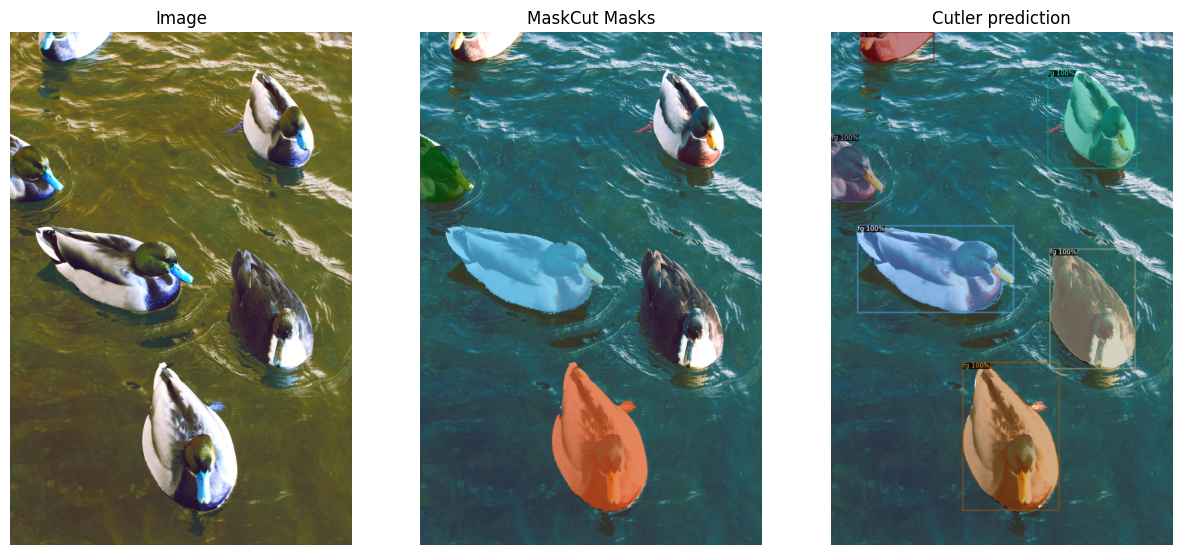
\includegraphics[width=1\textwidth]{Images/main/intro_cutler_pic.png}
	\caption[\textbf{Comparison of MaskCut and CutLER Outputs}]{\textbf{Maskcut and CutLER outputs}. Figure illustrates the outputs of MaskCut and CutLER with N=3 (Number of masks generated).}
	\label{fig:mask_cut_cutler_comparison}
\end{figure*}

\section{Overview of CutLER}
In the field of unsupervised object detection and instance segmentation, the recent work by Xudong Wang et al. introduces Cut-and-LEaRn (CutLER)~\cite{wang2023cut}, a novel approach that significantly advances the state-of-the-art. CutLER leverages the capabilities of self-supervised models to identify objects without human supervision, and it enhances this capability to train a high-performance localization model without any labeled data. The methodology begins with the MaskCut approach (inspired from~\cite{wang2022tokencut}), which generates coarse masks for multiple objects within an image. Subsequently, a detector is trained on these masks using a robust loss function. Performance is further improved through a self-training process where the model is iteratively trained on its own predictions. This approach not only simplifies the training process but also proves to be compatible with various detection architectures and capable of detecting multiple objects simultaneously. Figure~\ref{fig:mask_cut_cutler_comparison} shows original image, masks generated by Maskcut for N=3, where N represents maximum number of masks generated per image (Like in the original paper, we use N=3 in all of our experiments) and the final CutLER output.

The effectiveness of CutLER is demonstrated through extensive evaluations across diverse image domains, including video frames, paintings, sketches, and complex scenes. Notably, CutLER, utilizing a ResNet50 backbone, achieves a substantial performance increase, more than doubling the detection accuracy on 10 out of 11 benchmarks compared to the previous state-of-the-art method, FreeSOLO, which uses a ResNet101 backbone. Specifically, CutLER improves the average precision (AP50) by over 2.7 times across these benchmarks. This demonstrates CutLER's potential not only as a zero-shot unsupervised detector but also as an efficient low-shot detector, marking a significant step forward in unsupervised object detection and instance segmentation.

\section{Contribution and Key Insights}

This study focuses on the shortcomings of CutLER and the methods to minimize them. Our main contributions are:

\begin{enumerate}
%    \item \textbf{Analysis on the performance of different metrics for discriminating instances}: We compare the effectiveness of distance and similarity measures on discriminating instances of same and different classes.
    
    \item \textbf{Analysis on the influence of overlapping instances}: We compare the performance of the model when trained with and without overlapping instances and conclude that training without overlapping instances results in better instance discrimination.

    \item \textbf{Refining maskcut masks}: On top of self training, we refine mask-cut masks using CutLER predictions to remove noisy masks and retraining to yield better performance.
\end{enumerate}

% Wite about the improvement
%These contributions collectively elevate the understanding and practical implementation of GroupViT, opening doors to broader applications. Notably, the research achieves 18\% improvement on the training dataset, maintaining strong results on downstream datasets like PASCAL VOC and PASCAL Context.

\section{Outline}
\begin{itemize}
	 \item \textbf{Chapter \ref{chap:background}:}Explores the foundational concepts of Vision Transformers and attention mechanisms, with a detailed introduction to DINO features. Also covers the CutLER training pipeline and methods for mask refinement.
	 
    \item \textbf{Chapter \ref{chap:relatedwork}:} Explores recent advances in self-supervised feature learning and developments in unsupervised object detection and semantic segmentation.
    
    \item \textbf{Chapter \ref{chap:approach}:} Provides a detailed explanation of the limitations of CutLER, with descriptive examples of the proposed mask filtration method and the baseline approach. Also includes comprehensive background information for experimenting with the impact of overlapping instances.
    
    \item \textbf{Chapter \ref{chap:experiments}:} Details evaluation of the baseline and proposed methods across various datasets, focusing on instance detection and segmentation tasks. It includes a comparison of performance metrics, such as AP and AP50, highlighting improvements and differences between the methods. Additionally, it examines the impact of overlapping instances and discusses the effectiveness of the proposed mask refinement approach.
\end{itemize}
    \chapter{Background and Related Works}\label{chap:background}

\section{Vision Transformer}

\begin{figure}
	\centering
	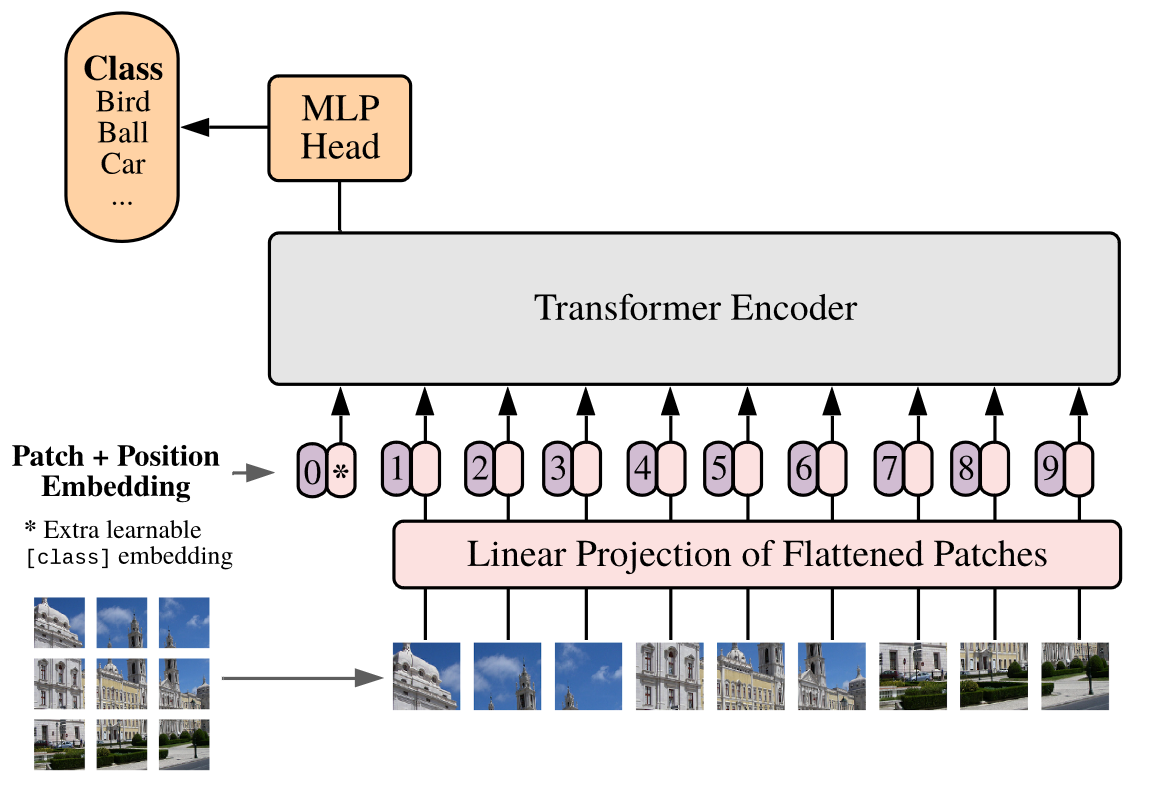
\includegraphics[width=0.9\textwidth]{Images/main/vit_full_arch.png}
	\caption[\textbf{ViT Architecture}]{\textbf{ViT Architecture}. ViT architecture from~\cite{dosovitskiy2020image}.}
	\label{fig:vit_full_arch}
\end{figure}

Vision Transformer (ViT), introduced by Dosovitskiy et al.~\cite{dosovitskiy2020image}, provides an alternative to Convolutional Neural Networks (CNNs) for image recognition, leveraging the transformer architecture to capture long-range dependencies and complex patterns that can complement and extend the capabilities of CNN-based models. The model applies Transformer architecture to image recognition tasks by treating image patches as sequences of tokens, akin to words in Natural Language Processing (NLP). The highlight of the paper is reusing the transformer encoder from the revolutionary work of Vaswani et al.~\cite{vaswani2023attentionneed} and adapting to use on images using patch tokenization and positional encoding.

As CutLER uses the features from a self-supervised ViT to generate masks, it is crucial to understand the basics architecture and working of ViT to get a complete picture of the feature generation process. Figure \ref{fig:vit_full_arch} shows the complete architecture of ViT. We are going to go into the main parts of the architecture for a better understanding of the process.

\subsection{Patch Tokens and Positional Encoding}

As each input is an image, unlike a sequence of words or tokens in~\cite{vaswani2023attentionneed}, the image is divided in fixed size patches (16x16 or 8x8) and each patch is treated as a token and each token is embedded into a fixed-dimensional vector using a learned embedding layer.

\begin{equation}
	\label{eq:pos_encoding}
	z⁰_i = z_i + p_i
\end{equation} 

For each token, instead of using sinusoidal position encodings~\cite{vaswani2023attentionneed} to retain information about the position of tokens in the sequence, a learnable position embedding is added as shown in the Eq.~\ref{eq:pos_encoding}, where \(p_i \in \mathbb{R}^{D}\) is the learnable position embedding for patch i. 

\begin{equation}
	\label{eq:full_pos_encoding}
	Z = [z_{class}; z⁰_1; z⁰_2;...; z⁰_N]
\end{equation}

Apart from \cite{vaswani2023attentionneed}, ViT~\cite{dosovitskiy2020image} introduces a special classification token \(z_{class}\) which is prepended to the sequence of patch embeddings. This token aggregates information from all patches and is used for the final classification task. The final encoding looks like Eq.~\ref{eq:full_pos_encoding}.

\subsection{Transformer Encoder}
The sequence of patch embeddings, augmented with positional information, is processed by the Transformer encoder. The encoder consists of multiple layers, each comprising Multi-Head Self-Attention (MSA) and Multi-Layer Perceptrons (MLPs), with Layer Normalization (LN) and residual connections. A weighted average~\cite{weng2020transformer} of individual attention outputs constitutes the final output. Figure~\ref{fig:transformer_encoder} illustrates the architecture of the transformer encoder. We briefly look into each part.

\begin{figure*}
	\centering
	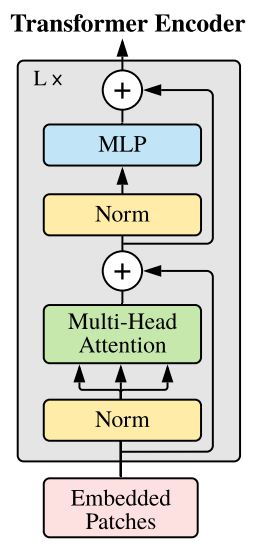
\includegraphics[width=0.3\textwidth]{Images/main/transformerblock.png}
	\caption[\textbf{Transformer Encoder Architecture}]{\textbf{Transformer Encoder Architecture}. Illustration of the Transformer encoder architecture in ViT~\cite{dosovitskiy2020image}.}
	\label{fig:transformer_encoder}
\end{figure*}

\subsubsection{Multi-Head Self-Attention (MSA)}
Self-attention allows the model to weigh the importance of different patches relative to each other.

\begin{subequations}
	\label{eq:qkv}
	\begin{align}
		\text{Queries  } Q = zW^{Q}_i \label{eq:query} \\
		\text{Keys  } K= zW^{K}_i \label{eq:key} \\
		\text{Values  } V = zW^{V}_i \label{eq:value}
	\end{align}
\end{subequations}

Given that \(d_k\) is the dimensionality of the key, query, and value vectors and \(W^Q_i, W^K_i, W^V_i \in \mathbb{R}^{D \times d_k }\) are learnable weight matrices, query, key, and value are computed as given in Eq.~\ref{eq:qkv}.


For each attention head \(i\),
\begin{equation}
	head_i =
	\text{Attention  }(Q_i,K_i,V_i) = \text{softmax  } \left(\frac{Q_iK^{T}_i}{\sqrt{d_k}}\right)V_i
\end{equation}

The outputs from all heads are concatenated and linearly transformed. Given \(W^O \in \mathbb{R}^{h-d_k \times D } \):
\begin{equation}
	MSA(z) = \text{Concat  }(head_i, head_2..., head_h)W^O
\end{equation}

\subsubsection{Layer Normalization and Residual Connections}
Each layer in the Transformer encoder includes Layer Normalization (LN) and residual (skip) connections
\begin{equation}
	z' = \text{MSA}(\text{LN}(z)) + z
\end{equation}
\begin{equation}
	z'' = \text{MLP}(\text{LN}(z')) + z'
\end{equation}
The Multi-Layer Perceptron (MLP) usually consists of two linear transformations with a Gaussian Error Linear Unit (GELU)~\cite{hendrycks2023gaussianerrorlinearunits} non-linearity in between. Assuming \(W_1\) and \(W_2\) are learnable weight matrices:
\begin{equation}
	\text{MLP}(x) = W_2(\text{GELU}(W_1x))
\end{equation}

\subsubsection{Output Layer}
The final output of the classification token is passed through a linear layer to produce the classification logits. Given \(C\) is the number of classes and \(W_{class} \in \mathbb{R}^{C \times D }\):
\begin{equation}
	\text{logits} = W_{class} \text{ }.\text{ } z''_{class}
\end{equation}
The linear layer projects the final representation of the classification token into the space of class labels.

\section{Self-Supervised Feature Learning}
Self-supervised feature learning is a crucial process that identifies patterns within extensive unlabeled datasets without the need for human-annotated labels. Plenty of research has been done in this field in the recent years. Several methods have been proposed, each with unique mechanisms and varying levels of success.

\subsection{Contrastive Learning}
Contrastive learning has gained significant attention for its effectiveness in self-supervised feature learning. One of the seminal works in this area is SimCLR~\cite{chen2020simple}. It employs a simple yet robust framework that leverages data augmentations to create positive pairs from the same image and negative pairs from different images. The model uses a contrastive loss to distinguish between these pairs, learning robust representations in the process. On the other hand, MoCo (Momentum Contrast)~\cite{he2020momentum} introduces a dynamic dictionary with a momentum encoder. This approach allows the model to maintain a queue of negative samples, effectively reducing memory requirements and improving scalability. Nevertheless, it still requires a substantial number of negative samples to function optimally and necessitates careful tuning of the momentum parameter to balance stability and learning efficiency.

\subsection{Clustering-Based Feature Learning}
Clustering-based feature learning approaches automatically uncover the natural groupings of data within the latent representation space. This clustering process helps in understanding the inherent structure of the data by grouping similar data points together based on learned features. Agglomerative Clustering with Self-supervision~\cite{asano2020selflabelling} can capture multi-scale structures and is found to be effective for diverse datasets. However, it is found to be computationally expensive and needs careful tuning of the self-supervised task. SwAV~\cite{caron2021unsupervised} combines clustering with contrastive learning by swapping assignments between different augmented views of the image. This method is efficient in terms of computational resources and achieves state-of-the-art performance on several benchmarks. But it is sensitive to the choice of hyperparameters.

\subsection{Distillation-Based Methods}
Distillation-based methods have also shown considerable promise in self-supervised learning. Bootstrap Your Own Latent (BYOL)~\cite{grill2020bootstrap} introduces a teacher-student network where the student learns to predict the teacher's representations. Remarkably, BYOL achieves this without using negative samples, simplifying the training process and reducing computational demands. However, it is sensitive to the choice of data augmentations and network architecture, and there is a potential risk of model collapse if not properly tuned. DINO~\cite{caron2021emerging} extends the self-distillation approach to Vision Transformers~\cite{dosovitskiy2020image}. DINO captures global image representations effectively without relying on negative samples. It shows strong performance on object detection and segmentation tasks, showcasing the potential of transformers in self-supervised learning.

Unlike traditional unsupervised representation learning methods that focus primarily on learning generalized visual features, our research centers on CutLER~\cite{wang2023cut}, which leverages these learned features, specifically DINO~\cite{caron2021emerging}, to focus on the task of instance detection. While CutLER builds upon the robust feature representations provided by DINO, it further enhances performance through advanced techniques and refinements.

\section{DINO}
The self-supervised model DINO, introduced by Caron, Mathilde, et al.~\cite{caron2021emerging}, achieves remarkable performance that rivals many state-of-the-art CNNs trained with supervision. DINO stands out for its ability to extract features that reveal clear information about semantic segmentation and scene layout within images. This capability distinguishes DINO from supervised ViTs and CNNs, underscoring its potential for sophisticated computer vision tasks without relying on annotated data.

As we will be using DINO features for producing the pseudo masks in CutLER~\cite{wang2023cut}, we need a basic understanding of DINO architecture and training.

\subsection{Knowledge Distillation}
 Knowledge distillation plays a crucial role in training a student model to mimic the behavior and representations learned by a teacher model, both of which are ViTs. 
 
\begin{figure*}
	\centering
	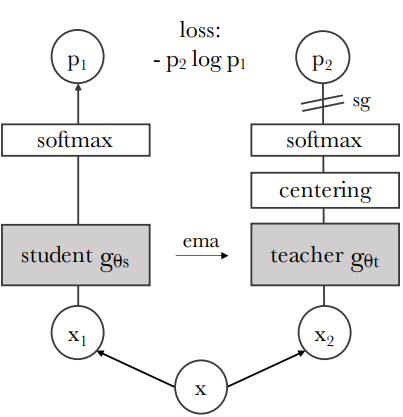
\includegraphics[width=0.5\textwidth]{Images/main/dino.png}
	\caption[\textbf{DINO Architecture }]{\textbf{Architecture of DINO} Illustration provided in~\cite{caron2021emerging}.}
	\label{fig:dino}
\end{figure*} 
 
 Initially, the teacher model is a ViT that is pre-trained on a large dataset using self-supervised learning techniques. The teacher captures rich, generalized features from the data. The student model is a smaller ViT that aims to replicate the teacher's performance but with fewer parameters, making it computationally lighter and potentially faster during inference.
 
\subsubsection{Momentum Encoder for Teacher}
Instead of using the teacher model directly, DINO employs a momentum encoder mechanism for stability and improved generalization. This means that the parameters of the teacher model are updated using a moving average of the student model's parameters, rather than directly during training.
\begin{equation}
	\label{eq:momentum}
	\theta_t \leftarrow m \theta_t + (1 - m) \theta_s
\end{equation}
The teacher model's parameters are updated using a momentum update rule as given in Eq.~\ref{eq:momentum}. Where \(\theta_t\) are the parameters of the teacher model, \(\theta_s\) are the parameters of the student model, and \(m\) is a momentum parameter (typically close to 1) that controls the rate of updating.

\subsection{Training Process}
DINO uses different augmentations of the same image to create multiple views. These augmented views are passed through both the teacher and student models. Outputs from both models are projected into a lower-dimensional space using projection heads. The optimization objective is to minimize the cross-entropy loss between the predicted probability distributions of the teacher and student models. Assume \(P_t(x)\) and \(P_s(x)\) represent the probability distributions predicted by the teacher and student models, respectively. The training process is illustrated in Fig.~\ref{fig:dino}.

\begin{equation}
	\label{eq:dino_objective}
	\min_{\theta_s} \mathcal{H}(P_t(x), P_s(x))
\end{equation}

The cross-entropy loss is computed between the softened distributions of the teacher and student models across all augmented views as given in Eq.~\ref{eq:dino_objective}.


\section{Unsupervised Object Detection and Instance Segmentation}
If we consider the recent methods for unsupervised object detection semantic segmentation, most of them leverage on self-supervised ViT~\cite{dosovitskiy2020image} features. In DINO~\cite{caron2021emerging} it is observed that the underlying semantic segmentation of images can be extracted using the saliency maps from the ViT. 

The quality of this segmentation surpasses existing methods when the image contains only a single instance. The effectiveness of DINO features in separating foreground and background has been affirmed by later works~\cite{engstler2023understanding}. Building on this observation, both LOST ~\cite{simeoni2021localizing} and TokenCut~\cite{wang2022tokencut} utilize DINO features to segment a single salient object from each image. These methods capitalize on the strength of DINO to construct a graph from the features of image patches. Unlike TokenCut and DINO, which can only detect one instance, LOST is capable of finding multiple instances within an image. However, it can't be used as a pre-trained model for down stream tasks. CutLER~\cite{wang2023cut} can not only detect multiple instances, but the model can also be further used as a pretrained model for label-efficient and fully-supervised learning.

MaskDistill~\cite{vangansbeke2022discovering} advocates a data-driven approach to mine object masks via self-supervised vision transformers and distill multiple object masks per image via an object segmentation model (Mask R-CNN~\cite{he2018maskrcnn}). Then a final segmentation model is trained using the found object masks. Although MaskDistill produces masks of similar quality to MaskCut, it generates only one class-agnostic mask per image. In contrast, MaskCut creates up to N masks per image to be used as pseudo labels. As a result, MaskCut has an advantage over MaskDistill in terms of quantity.

FreeSOLO~\cite{wang2022freesolo} and the follow up work Exemplar-FreeSOLO~\cite{Ishtiak_2023_CVPR} (with its addition of a randomly drawn pool of exemplars used in a contrastive learning loss) generate coarse segmentation masks with low guality and refine it further through self training similar to CutLER. But the poor quality of the coarse maps is a major drawback of this method, whereas CutLER masks made by the MaskCut~\cite{wang2023cut, wang2022tokencut} algorithm are usually better in quality and quantity than the initial masks used by MaskDistill~\cite{vangansbeke2022discovering} and FreeSOLO~\cite{wang2022freesolo}. 

Since CutLER outperforms other methods in most areas such as generating better pseudo ground truth masks, detecting multiple instances, and being compatible with various detection architectures, as well as serving as a pretrained model for supervised detection, our work primarily focuses on studying and enhancing the performance of CutLER.

\section{CutLER}
\begin{figure}
	\centering
	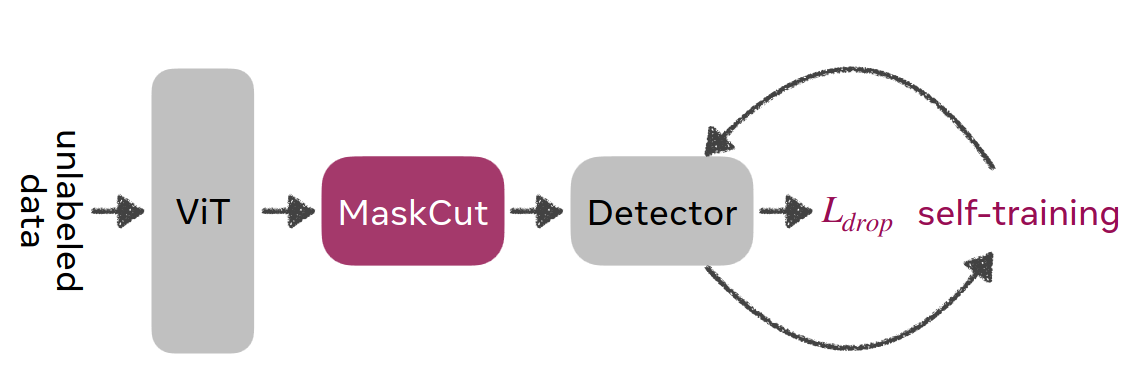
\includegraphics[width=0.8\textwidth]{Images/main/cutler_flow.png}
	\caption[\textbf{CutLER Overview}]{\textbf{CutLER Overview}. CutLER uses MaskCut for extracting coarse masks from the features of a self-supervised ViT. Following this, a detector utilizing a loss dropping strategy designed to be resilient against objects that MaskCut may overlook is used. Additionally, the model undergoes further enhancement through multiple rounds of self-training. Illustration taken from~\cite{wang2023cut}.}
	\label{fig:cutler_flow}
\end{figure} 

CutLER~\cite{wang2023cut} introduces a novel approach to address the challenges of object detection and instance segmentation in an unsupervised learning framework. By integrating Copy-Paste~\cite{ghiasi2021simplecopypastestrongdata} augmentation and a contrastive learning framework, the method not only circumvents the need for labeled data but also achieves state-of-the-art results in object detection and instance segmentation. The complete process is illustrated in Fig. \ref{fig:cutler_flow}.
 
\subsection{Normalized Cut}
Normalized Cut (NCut)~\cite{normcut} is a graph cut method where the goal is to partition an image into segments (or regions) by cutting a graph that represents the image, such that the similarity within each segment is maximized while the dissimilarity between different segments is also maximized. Understanding the NCuts algorithm is crucial, as CutLER's pseudo-ground truth masks rely on repeated NCuts to generate accurate masks. This process is key to CutLER's improved performance in unsupervised instance detection and segmentation.

In Normalized Cut, an image is represented as an undirected graph \( G = (V, E) \), where \( V \) is the set of nodes, each representing a pixel or a group of pixels and \( E \) is the set of edges, each representing a connection between two nodes, with weights \( w(i, j) \) indicating the similarity between nodes \( i \) and \( j \). A basic Cut is defined as the sum of the edge weights that are severed by the partition as given in Eq.~\ref{eq:cut}:

\begin{equation}
	\label{eq:cut}
	\text{Cut}(A, B) = \sum_{i \in A, j \in B} w(i, j)
\end{equation}

However, minimizing the cut alone tends to produce small, isolated segments. To address this, the Normalized Cut criterion is introduced. The Normalized Cut is defined as follows:

\begin{equation}
	\label{eq:norm_cut}
	\text{Ncut}(A, B) = \frac{\text{Cut}(A, B)}{\text{Assoc}(A, V)} + \frac{\text{Cut}(A, B)}{\text{Assoc}(B, V)}
\end{equation}

where \( \text{Assoc}(A, V) = \sum_{i \in A, j \in V} w(i, j) \) is the total connection from nodes in \( A \) to all nodes in the graph. The goal is to find the partition \( (A, B) \) that minimizes the NCut value. This can be expressed as an eigenvalue problem. The solution involves finding the eigenvector corresponding to the second smallest eigenvalue of the generalized eigenvalue problem given as Eq.~\ref{eq:eig_problem}.

\begin{equation}
	\label{eq:eig_problem}
	(D - W)x = \lambda D x
\end{equation}

where \( d(i) = \sum_{j} w(i, j) \) is the degree of node \( i \), and \( D \) is a diagonal matrix with \( d(i) \) on the diagonal and \( W \) is the weight matrix of the graph. The resulting eigenvector is used to partition the graph by thresholding its values.

\subsection{TokenCut}
TokenCut~\cite{wang2022tokencut} builds on the principles of Normalized Cut but adapts them to work within the framework of ViTs. Instead of operating on pixels, TokenCut segments an image by working with tokens - image patches processed by a ViT. In TokenCut, each token is treated as a node in a graph, and the edges are defined by the self-attention scores from the transformer, which capture the affinity between tokens. The goal remains similar: to partition the graph of tokens in a way that minimizes the NCut criterion. By leveraging the transformer’s attention mechanism, TokenCut can effectively capture global dependencies and segment objects in a self-supervised manner, even without labeled data. However, TokenCut only produces one mask per image, which limits the method from detecting multiple objects in an image. This issue is addressed in MaskCut.

\subsection{MaskCut}
\begin{figure}
	\centering
	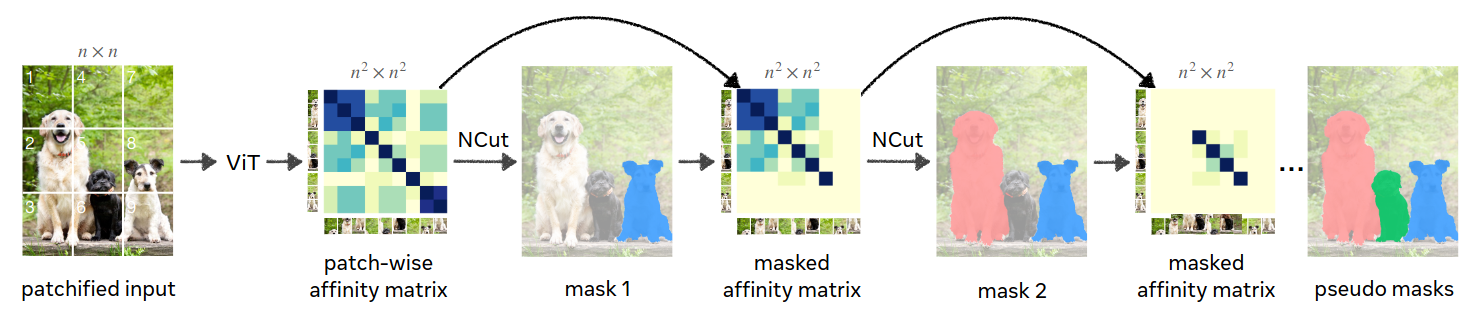
\includegraphics[width=1.0\textwidth]{Images/main/maskcut_eg.png}
	\caption[\textbf{MaskCut Flow}]{\textbf{MaskCut} works on the patch-wise
		similarity matrix for the image using a self-supervised DINO~\cite{caron2021emerging} model feature. N=3 defines the number of times NCut~\cite{normcut} is repeated on the background. In this case, 3 instances will be discovered per image in each step. Illustration taken from~\cite{wang2023cut}.}
	\label{fig:maskcut_flow}
\end{figure}

Like TokenCut~\cite{wang2022tokencut}, MaskCut considers the image segmentation problem as a graph partitioning task~\cite{normcut}. The nodes are tokens (each representing an image patch) and edges connect every pair of nodes, with weights \(W_{ij}\) reflecting the similarity between tokens. The optimization problem reduces the cost of dividing the graph into two sub-graphs, or a bipartition, by solving a generalized eigenvalue problem as given in Eq.~\ref{eq:eig_problem}. 

The similarity weight \( W_{ij} \) of NCut in TokenCut is based on the similarity of patches in the DINO feature space. Following recent methods~\cite{simeoni2021localizingobjectsselfsupervisedtransformers, vangansbeke2022discoveringobjectmaskstransformers, wang2023tokencutsegmentingobjectsimages}, they specifically employ the cosine similarity of 'key' features from the final attention layer of the DINO-pretrained model, represented as:

\begin{equation}
W_{ij} = \frac{K_i \cdot K_j}{\|K_i\|_2 \|K_j\|_2}
\end{equation}

where \( K_i \) denotes the 'key' feature of patch \( i \). They then solve Eq.~\ref{eq:eig_problem} to find the second smallest eigenvector \( x \). The main drawback of TokenCut is that it only uses the smallest eigenvector resulting in finding only one instance in the image. MaskCut overcomes this drawback and finds more instances by iteratively applying the same process in the background N times as given in Fig.~\ref{fig:maskcut_flow}. The figure shows the flow of MaskCut algorithm for N=3, where N defines the number of times NCut is repeated. In this case, up to 3 instances will be discovered per image.

Building on the work of~\cite{wang2023tokencutsegmentingobjectsimages, caron2021emergingpropertiesselfsupervisedvision}, a patch-wise similarity matrix for the image using features from a self-supervised DINO model~\cite{caron2021emerging} is created. Normalized Cuts~\cite{normcut} is applied to this matrix to obtain a single foreground object mask for the image. Subsequently, this foreground mask is used to mask out the affinity matrix values and repeat the process. This iterative approach enables MaskCut to identify multiple object masks within a single image.

MaskCut uses two conditions to improve the performance.
\begin{enumerate}
	\item An object centric prior~\cite{obj_centric_prior} is used to filter out backgrounds. ie, if the foreground contains more than 2 out of 4 corners, foreground and background are switched.
	
	\item From the intuition that foreground patches are more prominent than background ones~\cite{caron2021emergingpropertiesselfsupervisedvision, cond1_support_2}, we assert that the foreground mask should contain the patch corresponding to the maximum absolute value in the second smallest eigenvector.
\end{enumerate}
  If condition 1 is not satisfied and the current foreground contains two corners, background and foreground are switched.

\subsection{DropLoss}
A standard detection loss penalizes predicted regions \( r_i \) that do not overlap with the 'ground truth'. Since the ground truth masks from MaskCut may miss some instances, the standard loss does not allow the detector to identify new instances not labeled in the ground truth. To address this, the author proposes ignoring the loss for predicted regions \( r_i \) with minimal overlap with the ground truth.

\begin{equation}
	\label{eq:drop_loss}
L_{\text{drop}}(r_i) = \mathds{1}(\text{IoU}_i^{\text{max}} > \tau^{\text{IoU}}) L_{\text{vanilla}}(r_i)
\end{equation}

Specifically, during training, the loss is dropped for any predicted region \( r_i \) that has a maximum overlap of \( \tau^{\text{IoU}} \) with any ground truth instance as given in Eq. \ref{eq:drop_loss} where \(\text{IoU}_i^{\text{max}}\) denotes the maximum IoU with all ground truth for \( r_i \), and \( L_{\text{vanilla}} \) refers to the standard loss function for detectors. \( L_{\text{drop}} \) avoids penalizing the model for detecting objects missed in the 'ground truth', thus encouraging the exploration of different image regions.

\begin{figure}
	\centering
	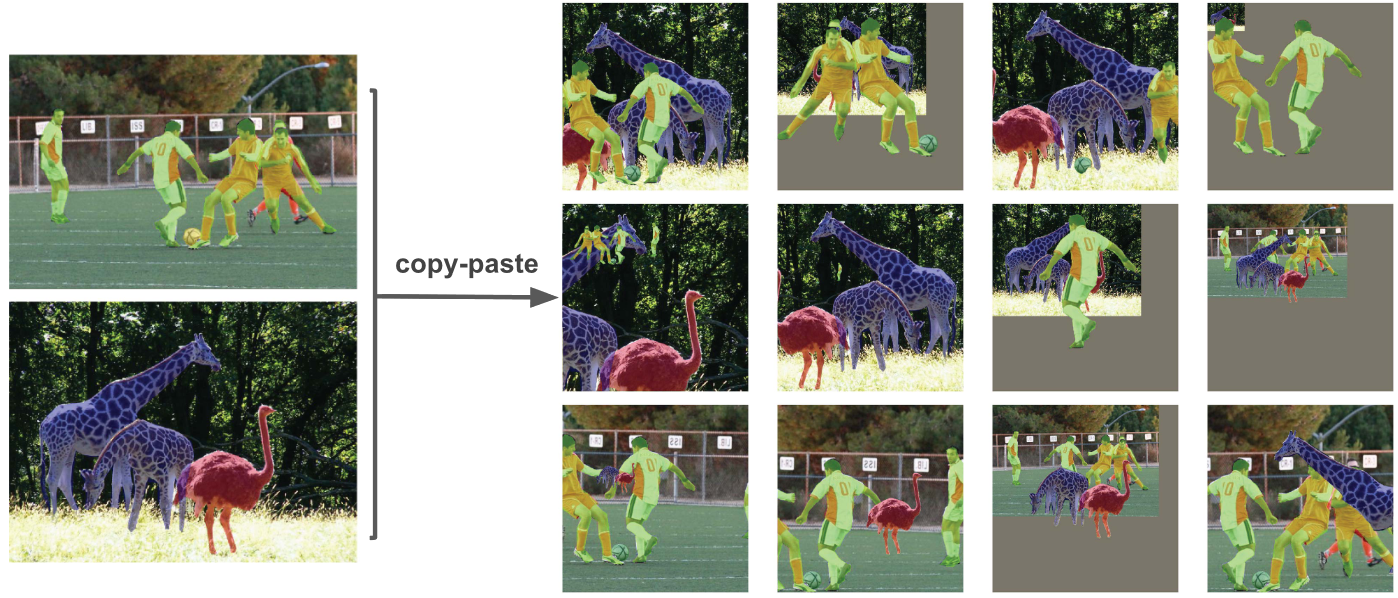
\includegraphics[width=1.0\textwidth]{Images/main/copy-paste.png}
	\caption[\textbf{Copy-Paste Augmentation}]{Illustration of Copy-Paste augmentation from~\cite{ghiasi2021simplecopypastestrongdata}.}
	\label{fig:copy_paste_aug}
\end{figure}

\subsection{Copy-Paste Augmentation}
Copy-Paste Augmentation~\cite{ghiasi2021simplecopypastestrongdata} is a data augmentation technique used to enhance the diversity of training datasets by artificially creating new training samples. This method involves copying objects from one image and pasting them onto another, thereby generating new training examples with diverse object placements and backgrounds as illustrated in Fig.~\ref{fig:copy_paste_aug}. The pasted objects can be resized, rotated, or otherwise manipulated to fit the new context. Lastly, the ground-truth annotations are also adjusted accordingly.

In Cutler, instead of using the standard copy-paste augmentation, where masks are rescaled with a factor between 0.8 and 1.25, masks are randomly downsampled with a scalar uniformly sampled between 0.3 and 1.0. This approach enables Cutler to recognize even smaller instances in the image effectively.

\subsection{Training}
The training process is divided into two stages: initial training followed by self-training, as depicted in Fig.\ref{fig:cutler_flow}. CutLER is agnostic regarding the choice of detector, allowing the use of any preferred detector. However, based on the experiments detailed in the paper, Cascade Mask R-CNN\cite{cai2019cascadercnnhighquality} yields better results compared to Mask R-CNN~\cite{he2018maskrcnn}.

First, pseudo-ground truth masks are generated using MaskCut for all images in Imagenet~\cite{deng2009imagenet} training set. The detector with a ResNet-50~\cite{he2015deepresiduallearningimage} backbone is trained using these pseudo-ground truth masks for 160K iterations with Copy-Paste augmentations and DropLoss.

\subsubsection{Self-Training}
\begin{figure*}
	\centering
	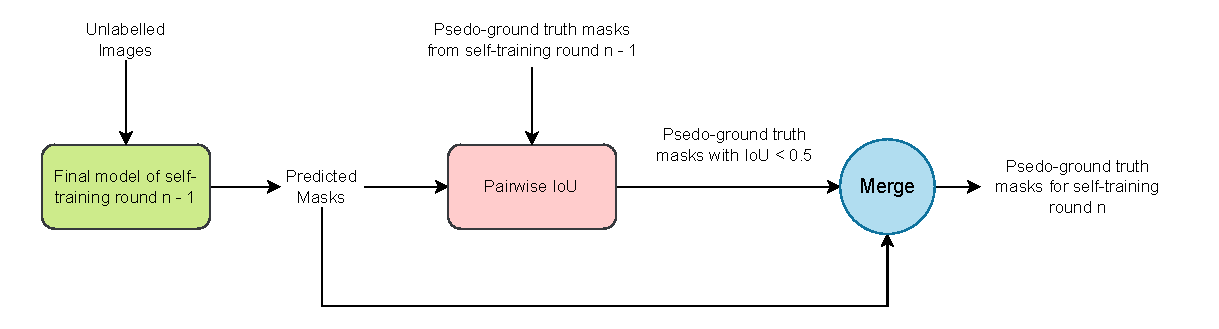
\includegraphics[width=1\textwidth]{Images/main/baseline_mask_filtration.pdf}
	\caption[\textbf{Mask Filtration Method in Baseline}]
	{\textbf{Mask Filtration in Baseline} before each self-training loop}
	\label{fig:baseline_mask_filtration_1}
\end{figure*}


To further improve the model performance, several self-training loops are also carried out. As depicted in the Fig.~\ref{fig:baseline_mask_filtration_1}, the pseudo-ground truth masks for the first round of self-training are formed by combining two sources. First, the CutLER mask predictions for each image with a confidence score greater than 0.7 are generated using the final model from the last training phase. Second, corresponding MaskCut masks that overlap less than 50\% with the predicted masks are included. Together, these masks form the pseudo-ground truth for the next phase. The mask refinement method is further explained in Section~\ref{section:bg_mask_refinement}.

The same process is repeated for the following self-training rounds except that instead of MaskCut masks, pseudo-ground truth masks of the previous stage are used to compare with predicted masks. Each self training round consists of 80K rounds and does not use DropLoss as we obtain comparatively good quality masks in the first round itself. The detailed information about the training with Figures is explained later in Section~\ref{section:Mask-Filtration} and~\ref{section:implementation_details}.

\subsection{Mask Refinement in CutLER}
\label{section:bg_mask_refinement}
The presence of incorrect masks in pseudo-ground truth can lead to overfitting on incorrect patterns or failure to generalize properly across different instances. To mitigate these issues, techniques like iterative refinement, robust loss functions, and the incorporation of consistency constraints have been proposed. Tang et al.~\cite{Tang_2018_CVPR} and Wang et al.~\cite{ziegler2022selfsupervisedlearningobjectparts} explore these approaches. 

Iterative refinement helps in progressively reducing this noise, leading to cleaner and more reliable labels~\cite{xie2020selftrainingnoisystudentimproves}. Popular refinement methods incorporate strategies like thresholding, where only high-confidence predictions are used for retraining, or use ensemble methods to combine predictions from multiple models for more reliable masks. CutLER also uses this approach.

In CutLER, before each self-training loop, 30 masks per image are generated for the entire Imagenet dataset using the latest trained model. Of these, masks are filtered based on the confidence score. In the paper, the masks with confidence score greater than \(0.7 - 0.05 * i\) on the \(i\) th iteration are kept and the rest are rejected. These filtered CutLER masks are compared with the corresponding MaskCut masks (in the first self-training round) or the pseudo-ground truth masks from the last round for each image. If the IoU between CutLER mask and MaskCut mask is less than 0.5, the corresponding MaskCut mask is added along with CutLER masks and this constitutes the pseudo-ground truth for the self-training loop.

The intuition is to retain masks from previous pseudo-ground truths that do not significantly overlap (i.e., overlap less than 0.5) with the current predictions. This strategy allows CutLER to explore new regions of the image that have not been thoroughly examined in previous iterations. However, a challenge with this approach is that it may perpetuate the inclusion of noisy masks in the ground truth during each self-training loop. Our approach seeks to address this issue by implementing a more refined method for removing the noisy background masks from the MaskCut masks and to improve the quality of the masks iteratively, which will be explained in detail in Section~\ref{section:proposed_method}.
    \chapter{Related Work}\label{chap:relatedwork}
%Give a brief overview of the work relevant for your thesis. 
\section{Self-supervised feature learning}
Self-supervised feature learning is a crucial process that identifies patterns within extensive unlabeled datasets without the need for human-annotated labels. Plenty of research has been done in this field in the recent years. Several methods have been proposed, each with unique mechanisms and varying levels of success.

\subsection{Contrastive learning}
Contrastive learning has gained significant attention for its effectiveness in self-supervised feature learning. One of the seminal works in this area is SimCLR\cite{chen2020simple}, It employs a simple yet robust framework that leverages data augmentations to create positive pairs from the same image and negative pairs from different images. The model uses a contrastive loss to distinguish between these pairs, learning robust representations in the process. On the other hand, MoCo (Momentum Contrast)\cite{he2020momentum} introduces a dynamic dictionary with a momentum encoder. This approach allows the model to maintain a queue of negative samples, effectively reducing memory requirements and improving scalability. Nevertheless, it still requires a substantial number of negative samples to function optimally and necessitates careful tuning of the momentum parameter to balance stability and learning efficiency.

\subsection{Clustering-based feature learning}
Clustering-based feature learning approaches automatically uncover the natural groupings of data within the latent representation space. This clustering process helps in understanding the inherent structure of the data by grouping similar data points together based on learned features. Agglomerative Clustering with Self-supervision\cite{asano2020selflabelling} can capture multi-scale structures and found to be effective for diverse datasets. But found to be computationally expensive and needs careful tuning of the self-supervised task. SwAV\cite{caron2021unsupervised} combines clustering with contrastive learning by swapping assignments between different augmented views of the image. This method is efficient in terms of computational resources and achieves state-of-the-art performance on several benchmarks. But it is sensitive to the choice of hyperparameters.

\subsection{Distillation-based methods}
Distillation-based methods have also shown considerable promise in self-supervised learning. BYOL (Bootstrap Your Own Latent)\cite{grill2020bootstrap} introduces a teacher-student network where the student learns to predict the teacher's representations. Remarkably, BYOL achieves this without using negative samples, simplifying the training process and reducing computational demands. However, it is sensitive to the choice of data augmentations and network architecture, and there is a potential risk of model collapse if not properly tuned. DINO\cite{caron2021emerging}, extends the self-distillation approach to Vision Transformers\cite{dosovitskiy2020image}. DINO captures global image representations effectively without relying on negative samples. It shows strong performance on object detection and segmentation tasks, showcasing the potential of transformers in self-supervised learning.

Unlike these unsupervised representation learning efforts, our research revolves around CutLer\cite{wang2023cut}, which focuses on automatically identifying natural pixel groupings and detecting instances within each image.

\section{Unsupervised object detection and instance segmentation}
If we consider the recent methods for unsupervised object detection semantic segmentation, most of them leverage on self-supervised Vision Transformer(ViT)\cite{dosovitskiy2020image} features. DINO\cite{caron2021emerging} observes that the underlying semantic segmentation of images can be extracted using the saliency maps from the ViT. 

The quality of this segmentation is superior to the existing methods if the image contains only is one instance. The superiority of DINO features to separate foreground and background has been affirmed by later works\cite{engstler2023understanding}. Building on this observation, both LOST \cite{simeoni2021localizing} and TokenCut \cite{wang2022tokencut} utilize DINO features to segment a single salient object from each image. These methods capitalize on the strength of DINO to construct a graph from the features of image patches. Unlike TokenCut and DINO, which can only detect one instance, LOST is capable of finding multiple instances within an image. But it can't be used as a pre-trained model for down stream tasks. But CutLer\cite{wang2023cut} not only can detect multiple instances, the model can be further used as a pretrained model for label-efficient and fully-supervised learning.

FreeSOLO\cite{wang2022freesolo} and the follow up work Exemplar-FreeSOLO\cite{Ishtiak_2023_CVPR} (with its addition of a randomly drawn pool of exemplars used in a contrastive learning loss) generates coarse segmentation masks with low guality and refines it further through self training similar to Cutler. But the poor quality of the coarse maps is a major draw back of this method, where as CutLer masks made by the MaskCut\cite{wang2023cut, wang2022tokencut} algorithm are usually better in quality and quantity than the initial masks used by MaskDistill\cite{vangansbeke2022discovering} and \cite{wang2022freesolo}. Even though Maskdistill produces similar quality masks compared to MaskCut, as it only produces one class agnostic mask per image and MaskCut produces N fixed number of masks per image to use as pseudo labels, MaskCut weighs over Maskdistill in quantity.

As CutLer dominates in most cases, including producing better pseudo ground truth masks, ablility to detect multiple instances, compatibility with various detection architectures, usable as pretrained model for supervised detection, our work would mostly focus on studying and improving the performance of CutLer.

\section{Semi-supervised object detection and instance segmentation}
In the realm of unsupervised semantic segmentation, the challenge of acquiring dense annotations has spurred innovative research efforts. Addressing this constraint, a series of studies \cite{hwang2019segsort,melas2022deep,cho2021picie,wang2022tokencut,hamilton2022unsupervised} have delved into harnessing self-supervised learning techniques to cultivate feature representations capable of supporting segmentation without necessitating extensive annotation efforts. Particularly, the DINO self-supervised model has illuminated that features extracted from its deep layers exhibit noteworthy correlation patterns congruent with genuine semantic labels. This insight has spurred further investigation. Drawing from this, Hamilton et al. introduced STEGO, which employs contrastive loss to distill pre-trained unsupervised visual features into semantic clusters, thus achieving compelling unsupervised segmentation results \cite{hamilton2022unsupervised}. Furthermore, Melas-Kyriazi et al. leverage spectral clustering on deep unsupervised representations, achieving state-of-the-art performance while also capitalizing on the informative features derived from DINO's architecture. Further This growing body of work showcases the potential of self-supervised methods, especially those rooted in DINO, to advance the landscape of unsupervised semantic segmentation \cite{melas2022deep}.
% \todo{see if you included all literature work for Vision Transformer for Semantic Segmentation}
% \todo{ add little bit about Hierarchical Vision Transformer for say swin, satrt with where all hierarchy in transformer have been explored and in semnatic segmentation where all it fanne dout well}
% \todo{Then in the the section say a very little about groupVit and that you would be moving on to that and our ork builds on that }

% \section{Visual Grouping}

% \section{Visual Language Pretraining}
% Vision-language pretraining has emerged as a powerful paradigm, driving advancements in the intersection of vision and language understanding. By jointly modeling visual and textual modalities, these pretrained models have revolutionized a range of vision-language tasks. Vision-language pretraining involves training a joint model on a vast corpus of image and text data. By learning from the paired visual and textual information, the model gains a comprehensive understanding of the cross-modal relationships between images and their associated captions or descriptions. 

% Explain the math and notation.
    \chapter{Approach}\label{chap:approach}

In the field of unsupervised instance detection and segmentation, CutLER~\cite{wang2023cut} gives a strong performance by exploiting a object-centric prior by training on ImageNet~\cite{deng2009imagenet}, as most images contain a single
object in the center of the frame.  Due to its strong instance discrimination abilities, CutLER is the current state-of-the-art method for this task.

In this chapter, we are exploring the limitation of CutLER, looking deeper into the special cases where CutLER fails such as overlapping instances and complex backgrounds. From the drawbacks of CutLER, we propose to train the model without overlapping instances, observing that overlapping instances are one of CutLER's main failure cases. We also investigate the hypothesis that a major reason for the better performance of CutLER is it's object-centric prior. Furthermore, using the gathered information from the observations, we introduce a hypothesis to refine MaskCut masks using CutLER predictions to train the model from scratch to obtain a better evaluation score across a variety of datasets.

\section{Assessing the Limitations of CutLER}
Even though CutLER is the state-of-the-art model for unsupervised instance detection and segmentation, it still has several drawbacks. Mainly We go through some of them in this section.

\subsection{Dependence on Initial Masks}
\begin{figure*}
	\centering
	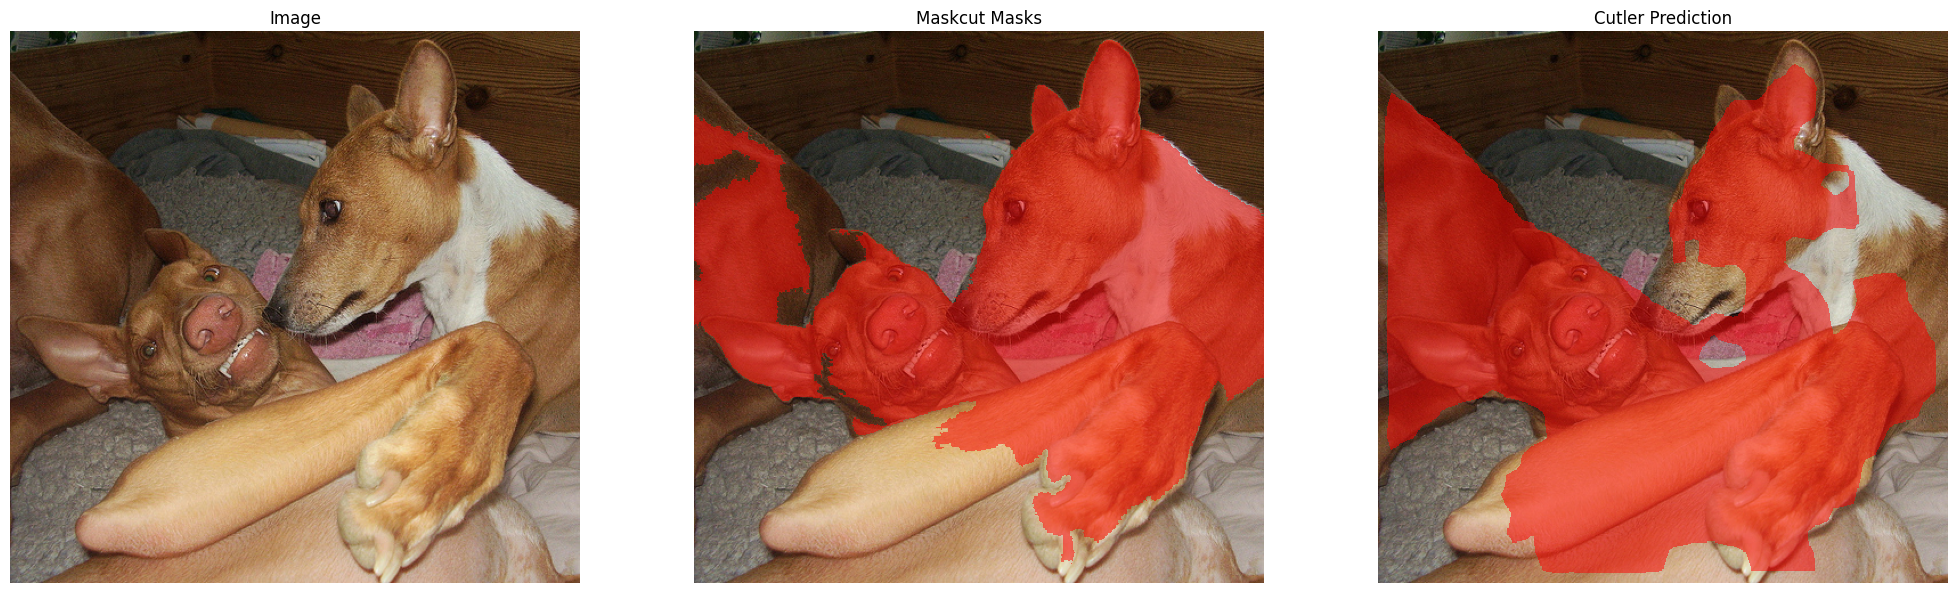
\includegraphics[width=1\textwidth]{Images/main/cutler_problem_3.png}
	\caption[\textbf{Dependence on Initial Masks}]{\textbf{Dependence on initial masks} reflected on the final CutLER prediction}
	\label{fig:intial_mask_dependence}
\end{figure*}

CutLER relies on initial masks provided by MaskCut. If these initial masks are of poor quality, the performance of CutLER may be adversely affected. These pseudo-ground truths often contain inaccuracies due to imperfect initial segmentation, which can arise from factors like complex backgrounds, occlusions, and variations in object appearance. Such imperfections can mislead the model, causing it to learn incorrect features and boundaries, ultimately degrading the quality of instance detection and segmentation. As MaskCut produces the masks based on a hyperparameter N (maximum number of masks generated per image), it also influences the quantity and quality of the pseudo-ground truths.

In challenging scenarios with cluttered backgrounds, occlusions or low-quality images, MaskCut could produce noisy masks as in Fig.~\ref{fig:intial_mask_dependence} which can also affect the quality of CutLER predictions. One common method to filter out good masks is thresholding, which is used in the baseline and our approach during self-training.

%\begin{table}[htbp]
%	\centering
%	\resizebox{1\textwidth}{!}{%
%	\begin{tabular}{c|c|c|c|c|c|c}
%		\toprule
%		\textbf{Methods}               & \textbf{APbox50} & \textbf{APbox} & \textbf{ARbox100} & \textbf{APmask50} & \textbf{APmask} & \textbf{ARmask100} \\ \midrule
%		TokenCut (1 eigenvec.) & 5.2 & 2.6 & 5.0 & 4.9 & 2.0 & 4.4 \\ \midrule
%		TokenCut (3 eigenvec.) & 4.7 & 1.7 & 8.1 & 3.6 & 1.2 & 6.9 \\ \midrule
%		MaskCut (t = 3)        & 6.0 & 2.9 & 8.1 & 4.9 & 2.2 & 6.9 \\ \midrule
%		CutLER                 & 21.9 & 12.3 & 32.7 & 18.9 & 9.7 & 27.1 \\ \midrule
%	\end{tabular}%
%	}
%	\caption{Performance comparison of different methods on box and mask AP/AR metrics.}
%	\label{tab:performance_table}
%\end{table}

To address this issue before self training, in our approach, we filter the MaskCut masks using the CutLER predictions and train from scratch, assuming the learning from scratch using better quality masks could improve the performance of the model. The approach is explained in detail in Section~\ref{section:proposed_method}.

\subsection{Overlapping Instances}
\begin{figure*}
	\centering
	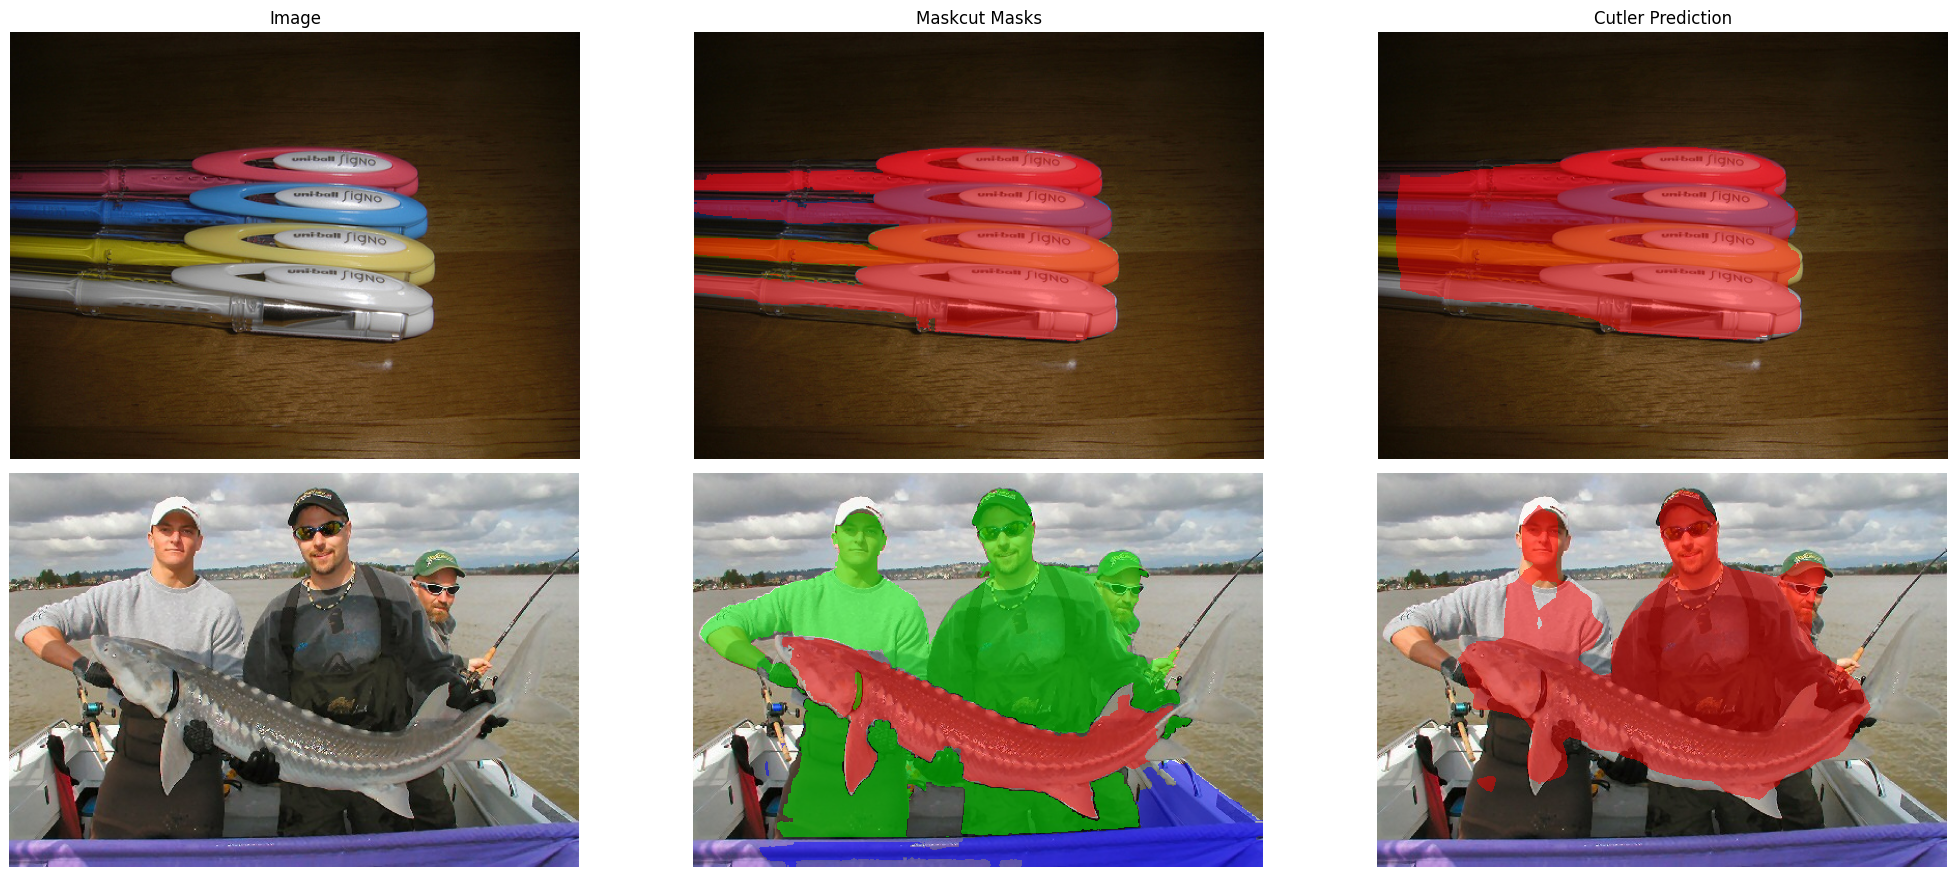
\includegraphics[width=1\textwidth]{Images/main/cutler-prob-overlap.png}
	\caption[\textbf{Cutler's Performance on Images with Overlapping Instances}]{\textbf{Grouping of overlapping instances} in MaskCut and CutLER outputs, which is a common problem in most of the existing unsupervised instance detection methods.}
	\label{fig:cutler_overlapping_instances_eg}
\end{figure*}

Identifying instances using unsupervised instance detection or segmentation methods present significant challenges, especially when instances are closely positioned or overlapping in an image. Overlapping objects often blend together, making it difficult for the model to accurately segment and differentiate them as distinct entities. This lack of explicit supervision complicates the model's ability to learn and generalize the spatial relationships and boundaries between objects.

\begin{figure*}
	\centering
	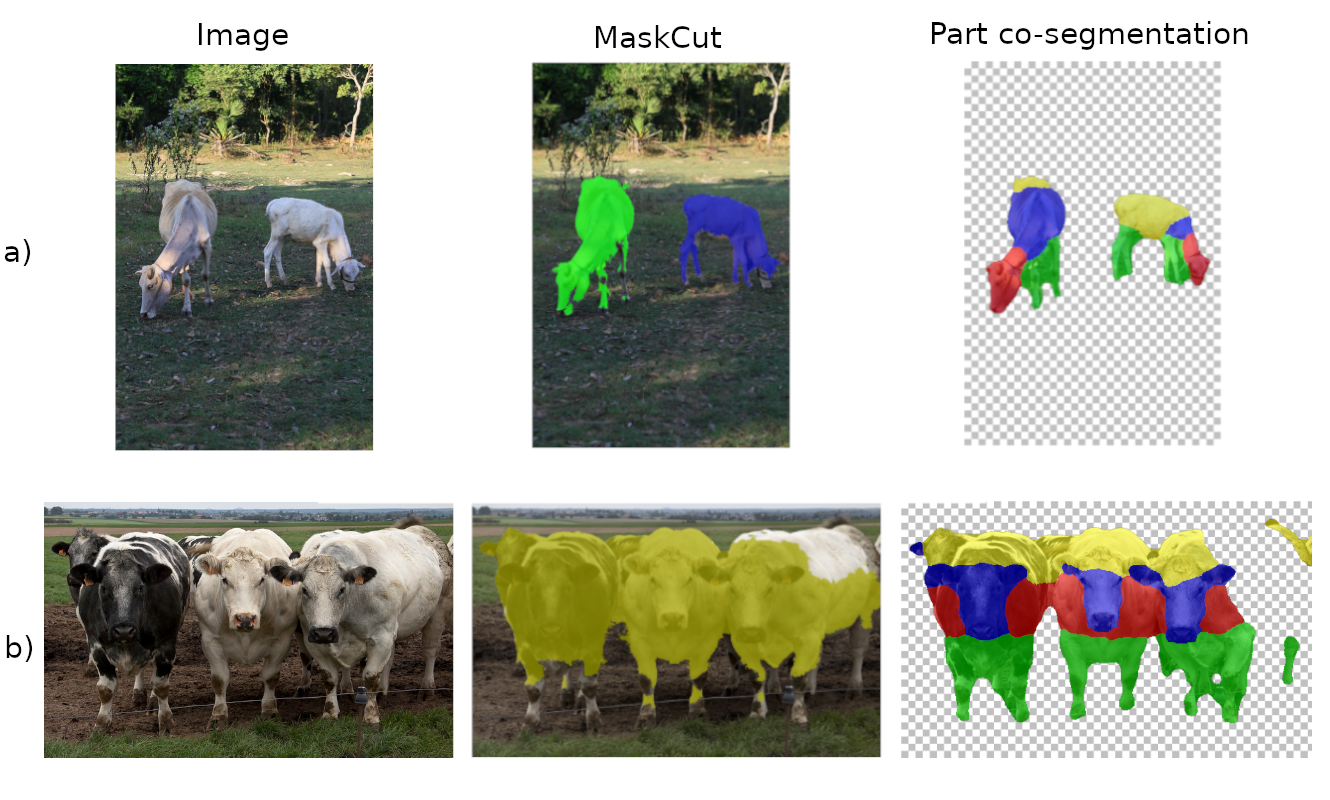
\includegraphics[width=1\textwidth]{Images/main/part-cosegm.png}
	\caption[\textbf{MaskCut vs Part Co-Segmentation Masks}]{\textbf{MaskCut vs Part Co-Segmentation Masks.} Discriminative features that could help differentiate instances are present in DINO features, as evidenced in n-part co-segmentation. But these features are not leveraged by MaskCut. }
	\label{fig:maskcut-instance-indifference}
\end{figure*}

As illustrated in Fig.~\ref{fig:cutler_overlapping_instances_eg}, in almost all cases of images with overlapping instances, MaskCut and CutLER groups those instances together. MaskCut primarily separates the foreground from the background rather than differentiating between individual instances~\cite{engstler2023understanding}. As a result, in Fig.~\ref{fig:cutler_overlapping_instances_eg}, it can successfully detect the fish but not the group of people as there is an overlap between them. Consequently, in images with overlapping instances, both MaskCut and CutLER generate outputs that are more akin to semantic segmentation than true instance segmentation.

MaskCut is also not effectively making use of the discriminative  DINO features that could help differentiate the instances. As it can be observed from Fig.~\ref{fig:maskcut-instance-indifference}, the part co-segmentation map generated by clustering feature maps obtained from the self-attention layers of DINO clearly contains features that could help discriminate these instances. However, MaskCut does not fully utilize these features. Instead, it operates more on a coarse level by segmenting the image into foreground and background regions. 

The problem is not exclusive to MaskCut or CutLER, but most of the existing methods~\cite{engstler2023understanding, cond1_support_2, Wang_2022_CVPR} also address this issue. Solving this problem requires devising an algorithm that could use the instance-discriminating representations from DINO and use it to separate the instances. We attempted to address this issue by using Keypoint Correspondences, which is a challenging task. As we could not come up with an graph-cut algorithm that fits problem, it is not a main part of this work. Nevertheless, it can be accessed in the Future Works Section~\ref{section:keypoint-correspondences}.

Another solution to address the grouping of instances would be to provide explicit semantic information of instances during training. It is explored in Wang et al. (2023)~\cite{wang2023cut} by testing with low-shot settings, ie, 2\% and 5\% labeled data, CutLER achieves 5.4\% and 7.3\% higher \(AP_{box}\) than the fully supervised MoCo-v2 with better separation of close and overlapping instances. But as our approach focuses solely on improving the unsupervised instance detection performance, the problem of grouping instances remains unsolved in our approach as well. But we intent to explore the influence of overlapping instances on CutLER training and evaluation which is explained in detail in the next section.

\subsubsection{Approach to Estimate the Impact of Overlapping Instances}
\label{section:analysis_ol_instancs}
%Based on the hypothesis that CutLER benefits from it's object-centric prior from training on Imagenet~\cite{engstler2023understanding}

Based on the observation that MaskCut often groups overlapping instances into a single mask, we hypothesize that training CutLER on ImageNet images without overlapping instances may improve performance compared to training on all images. This approach could reduce the number of inaccurate masks (removing grouped instance masks), improving the overall quality of pseudo-ground truth masks. Additionally, we aim to explore whether a model trained exclusively on non-overlapping instances can enhance detection of individual instances in images where overlaps occur.

For the sake of completeness and to observe whether there is any relative improvement or loss, we compare three approaches of training CutLER. 

\begin{enumerate}
	\item Using all images of ImageNet (Same as the baseline)
	\item Using images without any overlapping instances 
	\item Only using images with overlapping instances
\end{enumerate}

We expect that the model trained without overlapping instances will outperform the baseline, while the model trained exclusively on images with overlapping instances will likely underperform compared to the baseline. Splitting the evaluation dataset according to these three approaches should also reveal a similar performance pattern. Our hypotheses is supported by the positive results from the experiments in Section~\ref{section:overlapping-results}.

To test the hypothesis, we make use of ground truth bounding box annotations provided by ImageNet and the images with an overlap (IoU) of \(\tau > \text{0.1}\) is taken as the criteria to filter images for approach 2 and 3. As ImageNet contains mostly object-centric single instance images, the third approach (only using images with overlapping instances) would have significantly less number of training images compared to the other two approaches. Specifically, Approach 3 utilizes 6\% of the annotated ImageNet dataset, while Approach 2 uses the remaining 94\%. Given the significantly smaller training sample size in Approach 3, a fair comparison isn't possible. Therefore, we focus on Approach 2 for comparison with the baseline.

Through this approach, we expect to observe an improvement by using less training data. But using this method in unsupervised fashion is rather difficult. Due to the grouping of nearby instances, the process of filtering images with overlapping instance is extremely challenging. Hence these tests are carried out using bounding box labels of ImageNet. However, the approach gives insights on the influence of overlapping instances in training that can be useful for future research.

\subsubsection{Estimating the Impact of Object-Centric Instances}
\label{section:analysis_oc_instancs}
To support our hypothesis that an object-centric prior is a key contributor to CutLER's state-of-the-art performance, we propose that filtering out non-object-centric images from the training dataset could further enhance its effectiveness. Recent research has highlighted the significant role that object-centric images play in model performance~\cite{engstler2023understanding, Gasparim_2021}.
	
Object-centricity is hard to define. As we couldn't find a standard way to define object-centicity for our research~\cite{Russakovsky, Gasparim_2021}, we defined two simple hyperparameters to filter object-centric images.

\begin{itemize}
	\item \textbf{Area Threshold} : Minimum area ratio of bounding box to image
	\item \textbf{Center Threshold} : Maximum distance ratio from the image center to bounding box center to the image diagonal.
\end{itemize}

We set Area Threshold to 0.1 and Center Threshold to 0.2. That is, if bounding box has size less than 10\% of the size of the image or the distance between image center and bounding box center is more than 20\% of image's diagonal length, that image will be rejected from the training set.

Like in the previous section, to test the hypothesis, we make use of ground truth bounding box annotations provided by ImageNet. We are only using single instance images as object-centric images can contain overlapping instances as well. Due to the filtration process, we only use 77\% images of annotated ImageNet dataset, that is only 30\% of total ImageNet images. Even with this much less data, we expect to observe a competitive result compared to the baseline. 

\subsection{Images with Complex Background}
\begin{figure*}
	\centering
	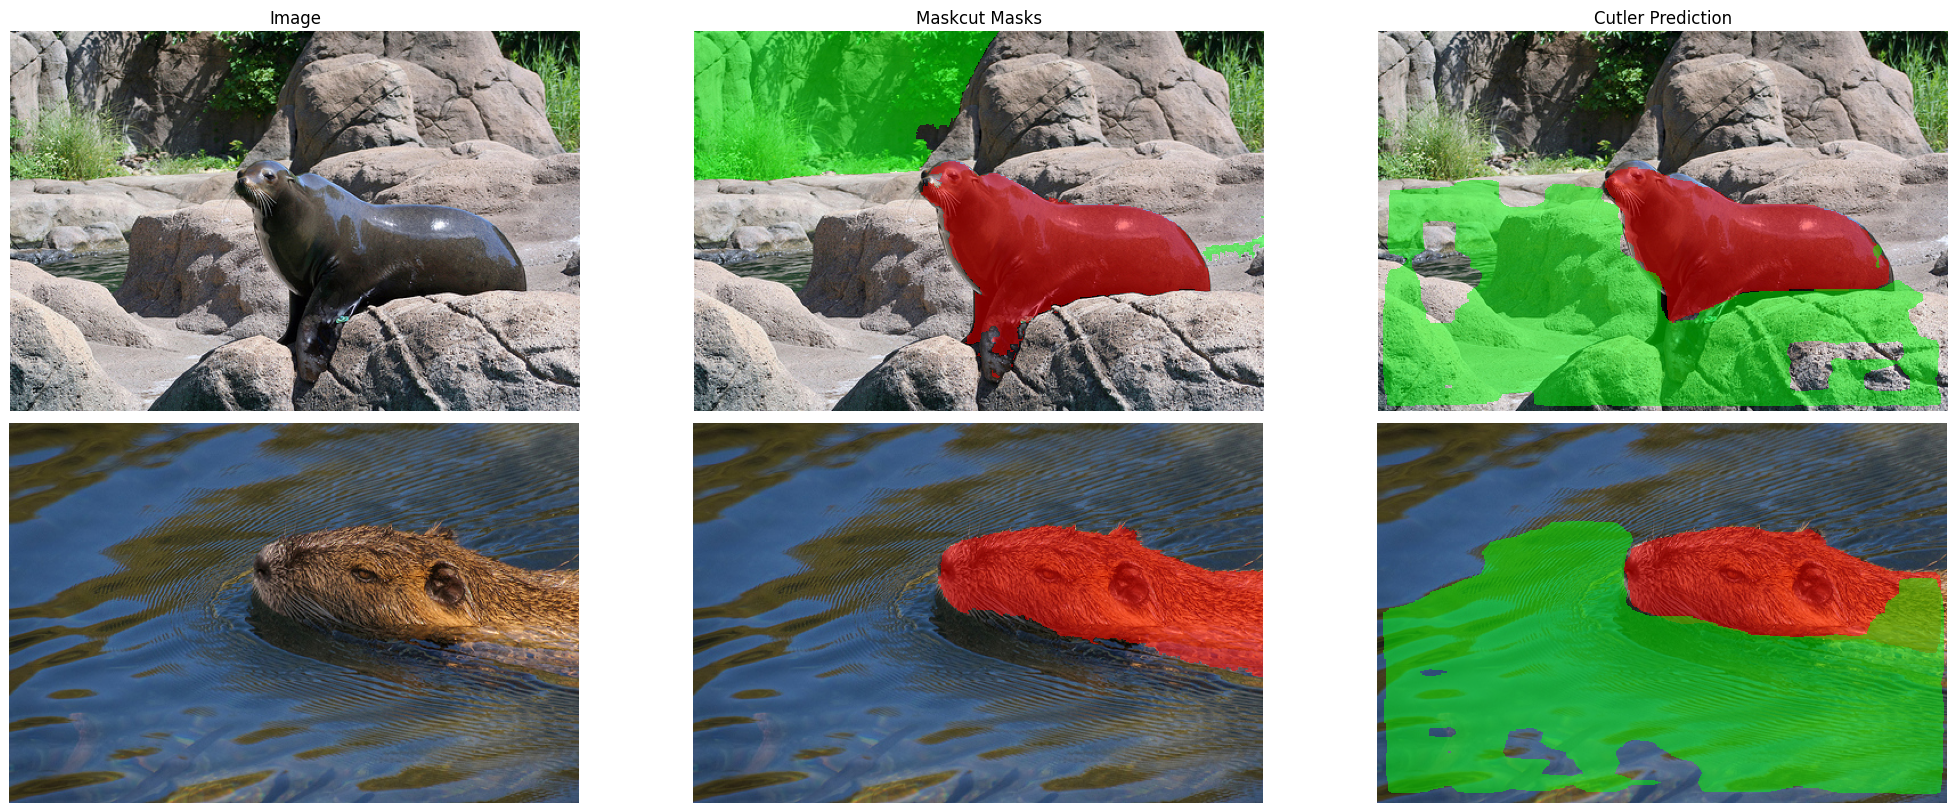
\includegraphics[width=1\textwidth]{Images/main/cutler-prob-noisy-bg.png}
	\caption[\textbf{Cutler's Performance on Images with Complex Background}]{\textbf{Images with complex backgrounds} impacting MaskCut and CutLER outputs, leading to undesired background mask generation}
	\label{fig:cutler_noisy_bg_eg}
\end{figure*}

Even though DINO features are good at providing foreground-background separation, images with complex or unusual backgrounds can possess challenges to this task. In our approach, we intent to address the issue of unwanted masks generated due to complex backgrounds as shown in Fig.~\ref{fig:cutler_noisy_bg_eg}. Such masks can not only be present in the MaskCut masks which act as the pseudo-ground truth for CutLER training, but also in the CutLER predictions itself. As per our observation, the mask filtration strategy used by the baseline doesn't address this issue, which is explained in detail in Section~\ref{sec:baseline_mask_filteration}.

In CutLER, a self-training loop is implemented to iteratively refine the pseudo ground truth masks. We hypothesize that removing undesired background mask before training and self-training phases could improve the performance of the model. We plan to test this hypothesis by modifying the mask filtration algorithm used to refine pseudo-ground truth masks in the baseline method before each self-training loop. This modified algorithm will be used to generate improved MaskCut masks, enabling us to train the model from scratch with better pseudo-ground truth. Our approach addressing this issue is explained in Section~\ref{section:Mask-Filtration}.

\section{Mask Filtration}
\label{section:Mask-Filtration}
Generating initial pseudo-ground truth masks using a pre-trained model or some heuristic methods may contain errors or inaccuracies. The presence of incorrect masks can lead to overfitting on incorrect patterns or failure to generalize properly across different instances. To mitigate these issues, techniques like iterative refinement, robust loss functions, and the incorporation of consistency constraints have been proposed. Tang et al.~\cite{Tang_2018_CVPR} and Wang et al.~\cite{ziegler2022selfsupervisedlearningobjectparts} explore these approaches. Iterative refinement helps in progressively reducing this noise, leading to cleaner and more reliable labels~\cite{xie2020selftrainingnoisystudentimproves}. Popular refinement methods incorporate strategies like thresholding, where only high-confidence predictions are used for retraining, or use ensemble methods to combine predictions from multiple models for more reliable masks.

\subsection{Baseline Mask Filtration Method}
\label{sec:baseline_mask_filteration}

\begin{figure*}
	\centering
	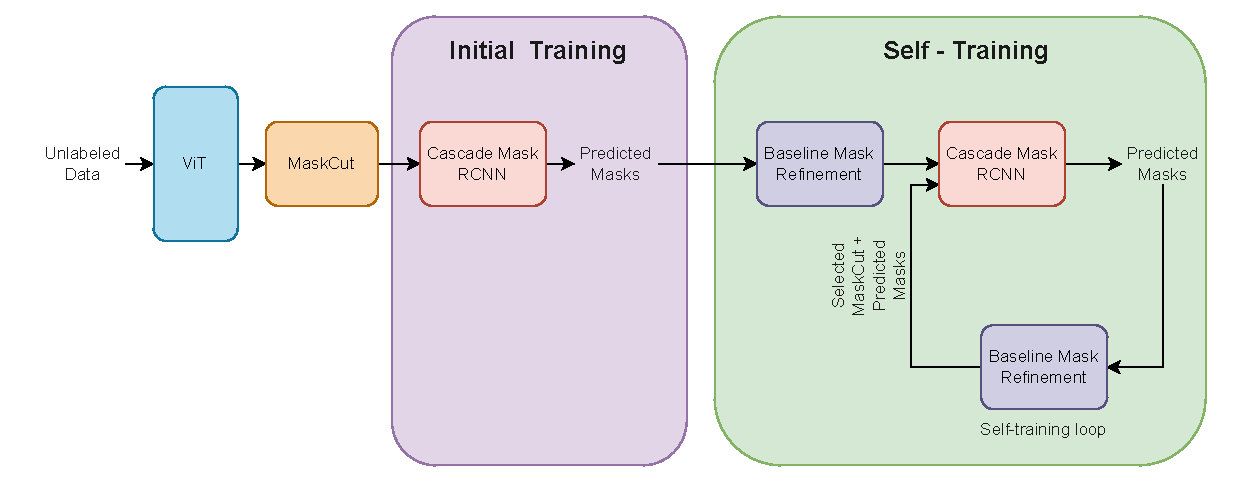
\includegraphics[width=1\textwidth]{Images/main/baseline_approach.pdf}
	\caption[\textbf{Baseline Training Pipeline}]{\textbf{Baseline training pipeline} with repeated mask filtration and self-training}
	\label{fig:baseline_training}
\end{figure*}

\subsubsection{Initial Training}
Initially, the detector (Cascade Mask RCNN) trained with  ImageNet dataset using MaskCut masks as pseudo-ground truth for 160K iterations with Copy-Paste augmentations and DropLoss. As illustrated in Fig.~\ref{fig:baseline_training}, after the initial training, the trained model predicts masks for each image in ImageNet dataset (30 masks per image) using the trained model. Out of the 30 predicted masks, high-quality ones are filtered by applying a confidence score threshold of 0.7 and passed onto the mask filtration pipeline. 

\begin{figure*}
	\centering
	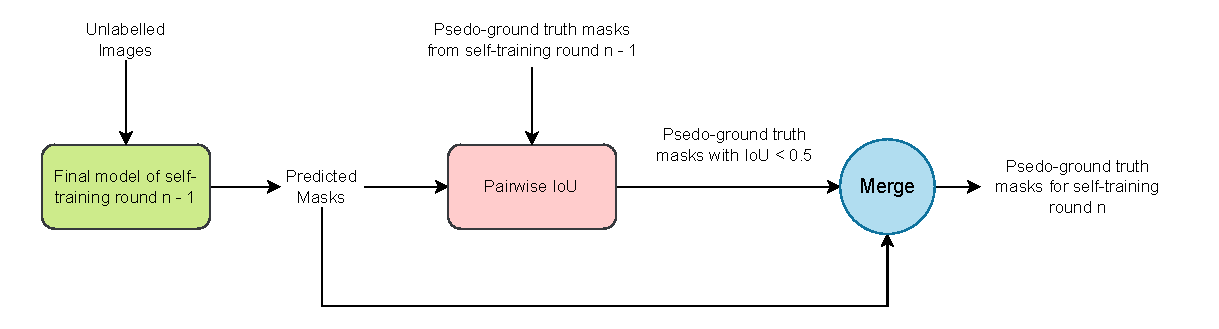
\includegraphics[width=1\textwidth]{Images/main/baseline_mask_filtration.pdf}
	\caption[\textbf{Mask Filtration Method in Baseline}]{\textbf{Mask Filtration in Baseline} before each self-training loop}
	\label{fig:baseline_mask_filtration}
\end{figure*}

\begin{figure*}
	\centering
	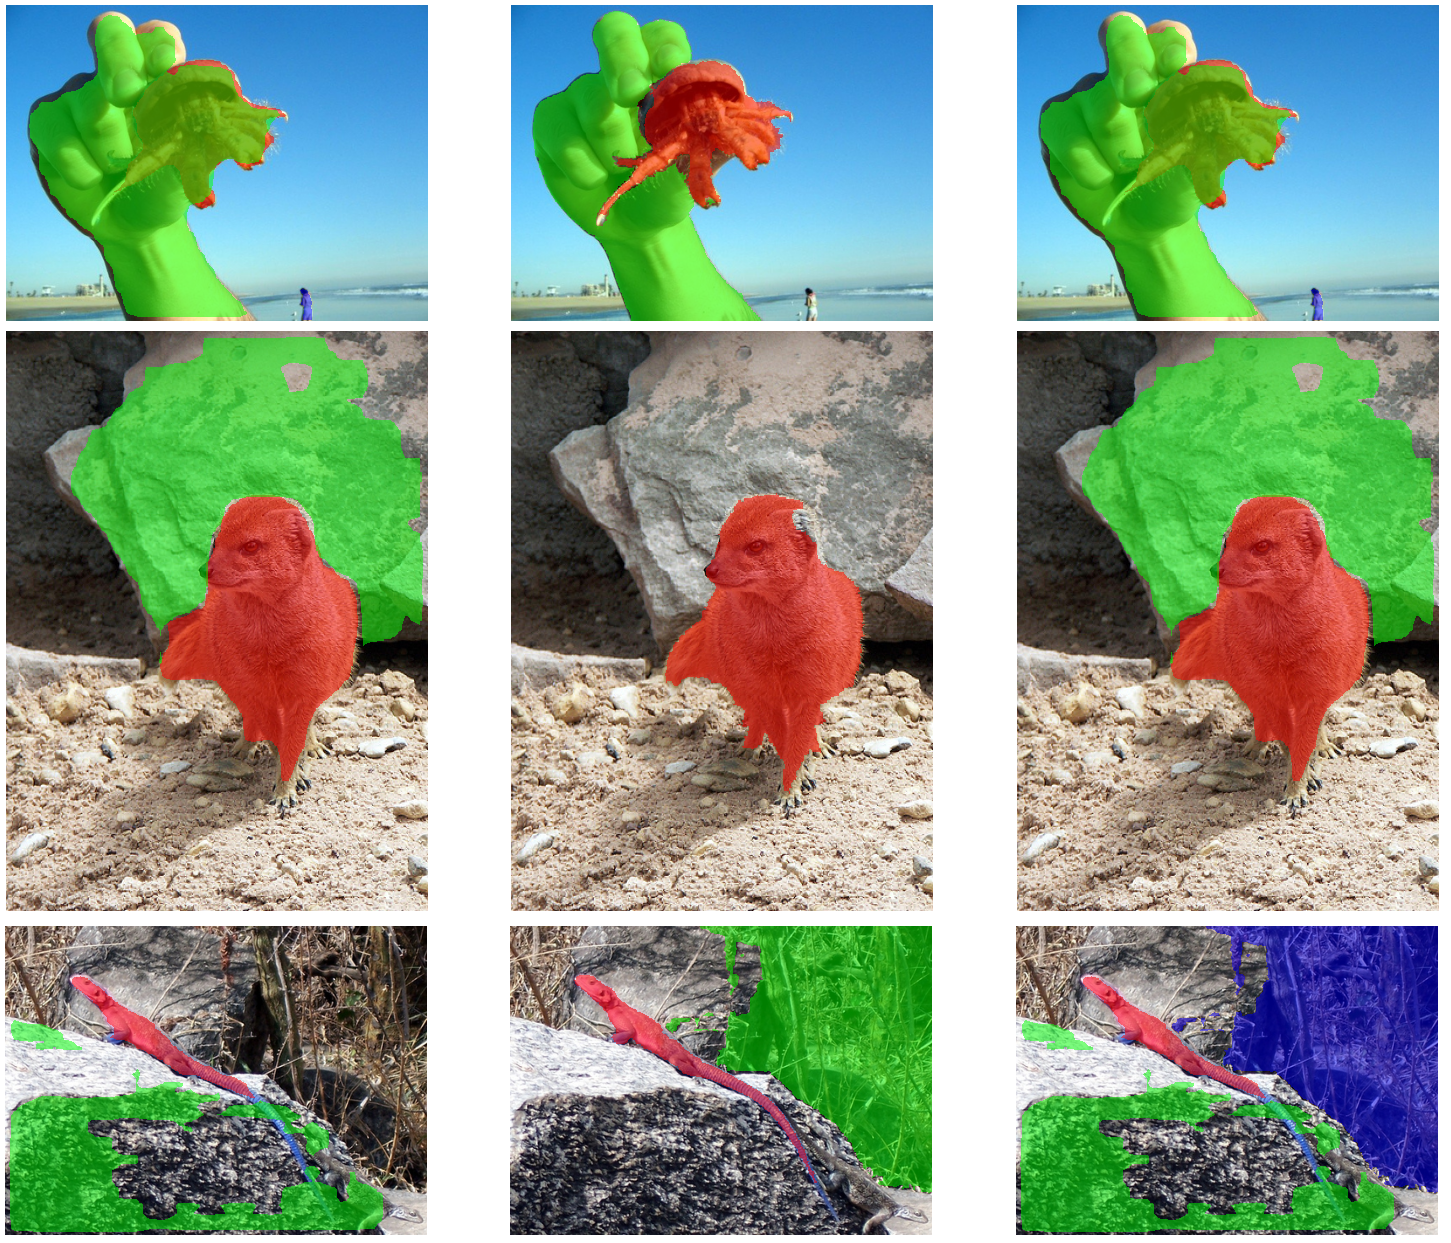
\includegraphics[width=1\textwidth]{Images/main/filtered_mask_problem.png}
	\caption[\textbf{Mask Filtration in Baseline - Qualitative Examples}]{\textbf{Mask Filtration in Baseline - Qualitative Examples} Examples illustrates CutLER prediction masks, MaskCut masks and masks selected by CutLER mask filtration method (left to right)}
	\label{fig:filtered_mask_problem}
\end{figure*}

\subsubsection{Mask Filtration and Self-Training}
Baseline mask filtration process is illustrated in Fig.~\ref{fig:baseline_mask_filtration}.  Pairwise IoU is calculated between the selected predicted masks and MaskCut masks. For mask pairs with an IoU below 0.5, the corresponding MaskCut masks are included, along with all selected predicted masks, to form the pseudo-ground truths for the next self-training stage. Intuitively, MaskCut masks that have less than 50\% overlap with the selected predicted masks are included alongside the CutLER masks to form pseudo-ground truths for next self-training round. 

The goal is to retain as many non-overlapping masks as possible. However, always including masks that don't overlap with CutLER prediction masks can introduce irrelevant or unwanted masks into the pseudo-ground truth. This can affect the performance of the model.

For further self-training loops, the same procedure repeats, except that instead of MaskCut masks, pseudo-ground truth masks of the last round are used to compare with the predicted CutLER masks. Performance of the model claims to have improved upto 3 self-training loops by the authors. We will be running 2 self-training loops for both the baseline and proposed method in our experiments.

\subsubsection{Qualitative Examples}
Figure~\ref{fig:filtered_mask_problem} illustrates some qualitative examples of how the baseline filters masks for the next round of training. Despite having either good MaskCut mask or CutLER prediction, baseline selects large incorrect MaskCut masks which doesn't overlap much along with CutLER prediction masks, which adversely affect the model performance. We intent to remove these false masks to generate better quality pseudo-ground truths.


\subsection{Proposed Mask Filtering Method}
\label{section:proposed_method}

\begin{figure*}
	\centering
	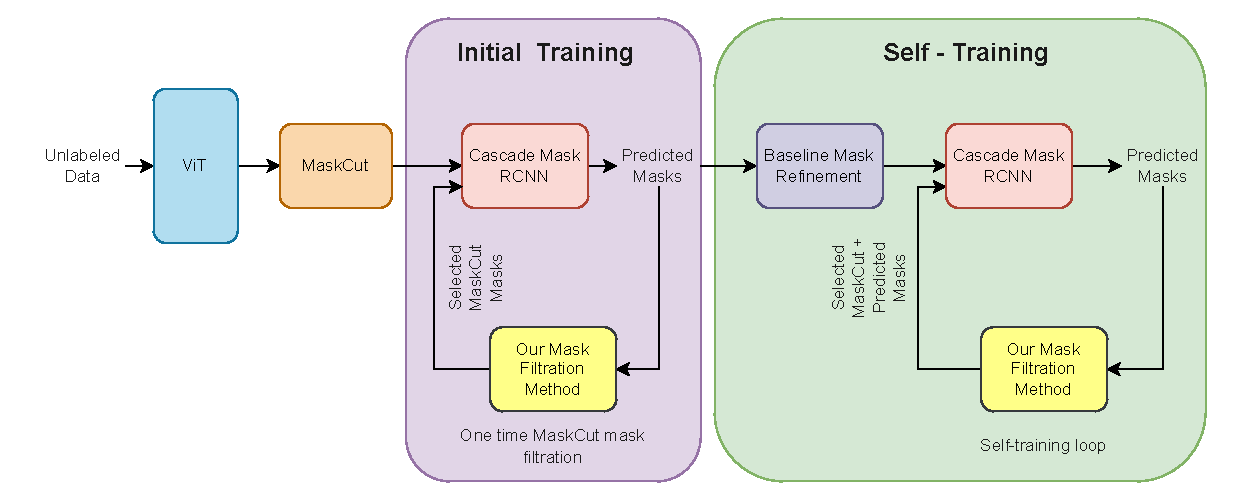
\includegraphics[width=1\textwidth]{Images/main/proposed_method_last.pdf}
	\caption[\textbf{Proposed Training Pipeline}]{\textbf{Proposed Training Pipeline} featuring a one-time MaskCut mask filtration followed by multiple self-training loops with our mask filtration method.}
	\label{fig:proposed_training}
\end{figure*}
Emphasizing quality over quantity, we introduce an improved approach for mask filtration. Noting that the current mask filtration method in CutLER tends to include unwanted background masks in its pseudo ground truths, we propose to enhance the process by removing ambiguous masks from the ground truth instead of retaining them. This adjustment aims to improve the overall quality and reliability of the pseudo ground truths, leading to better model performance.

\subsubsection{Initial Training}
\begin{figure*}
	\centering
	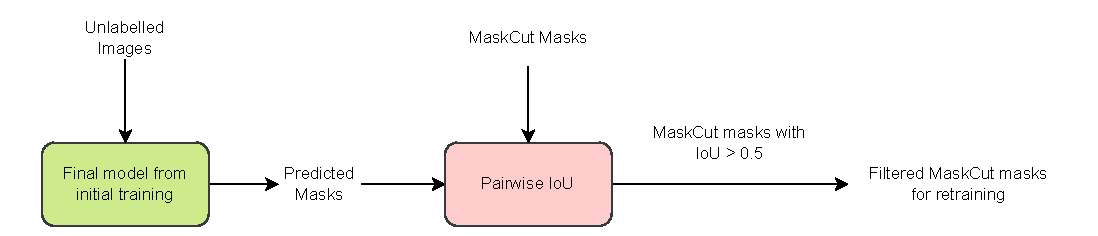
\includegraphics[width=1\textwidth]{Images/main/our_mask_filtration_1.pdf}
	\caption[\textbf{Mask Filtration in Proposed Method}]{\textbf{Mask Filtration in Our Method}, used to filter MaskCut masks after the initial training.}
	\label{fig:our_mask_filtration}
\end{figure*}

As illustrated in Fig.~\ref{fig:proposed_training}, we train the detector for 160K iterations using Copy-Paste augmentations and DropLoss identical to the baseline. After which we introduce an additional step to refine MaskCut masks. This refinement involves preserving only high-certainty masks by comparing them against CutLER predictions.

\subsubsection{Proposed Mask Filtration and Retraining}
Proposed mask filtration method is illustrated in Fig.~\ref{fig:our_mask_filtration}. After the first training phase, like in the baseline, high-quality predicted masks are filtered by applying a confidence score threshold of 0.7.  Instead of creating the new pseudo-ground truth by selecting masks from both MaskCut masks and CutLER prediction masks, we focus solely on filtering MaskCut masks. Rather than selecting MaskCut masks corresponding to mask pairs with an IoU < 0.5 from the batch IoU matrix, we choose MaskCut masks that correspond to mask pairs with an IoU > 0.5. 

The idea is to filter highly certain MaskCut masks and discard possible incorrect masks. This selected MaskCut masks are treated as the new pseudo-ground truth and we train from scratch for 160K iterations with Copy-Paste augmentations and DropLoss. We are effectively repeating the same initial training process, but with better masks. With the filtered high quality masks in hand, we expect to achieve a better performance. 

It’s important to note that if no masks are selected for an image, that image is removed from the training set, resulting in a smaller dataset and reducing the training time (Around 130K images are dropped from ImageNet during this stage). This approach effectively eliminates potentially unwanted masks from the pseudo-ground truth, possibly providing more accurate mask predictions.

\subsubsection{Further Mask Filtration and Self-Training}
\label{section:proposed_mask_filtration_self_training}
\begin{figure*}
	\centering
	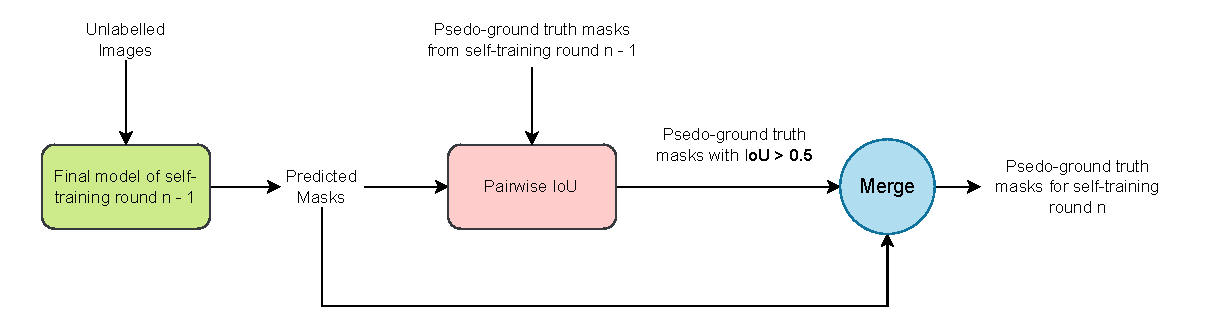
\includegraphics[width=1\textwidth]{Images/main/our_filtration_self_training.pdf}
	\caption[\textbf{Mask Filtration in Proposed Method During Self-Training}]{\textbf{Mask Filtration in Proposed Method}, used to filter masks during self-training.}
	\label{fig:our_mask_filtration_self_training}
\end{figure*}


 For self-training, we follow training pipeline of the baseline, training for 80K iterations are without using DropLoss. We use our mask filtration method illustrated in Fig~\ref{fig:our_mask_filtration_self_training} to filter masks between self-training rounds. 
 
 The only modification to the baseline approach is selecting pseudo-ground truth masks with IoU > 0.5 with predicted masks, rather than those with IoU < 0.5. This way, we always retain masks with high certainty. But this also restricts the exploration. Limiting pseudo-ground truth labels to only high-confidence masks could constrain improvements in the self-training round. 
 
 %This intuition is validated by our experiments in Section <secno>.
 
 %We use baseline filtration method during self-training. As we already have finer masks, refining further might lead to over-fitting. Limiting pseudo-ground truth labels to only high-confidence masks (like in our filtration method) could constrain improvements in the self-training round. Hence baseline filtration
 
By utilizing a smaller number of more accurate masks, we anticipate an improvement in precision. However, there may be a slight decrease in recall if the reduced number of masks does not sufficiently cover all ground truth instances. But our experiments indicate that this change is negligibly small. Detailed results and analysis on this can be found in the Section~\ref{section:persistant_recall}.



%\begin{figure*}[h]
%	\centering
%	\begin{subfigure}[b]{0.47\textwidth}
%		\centering
%		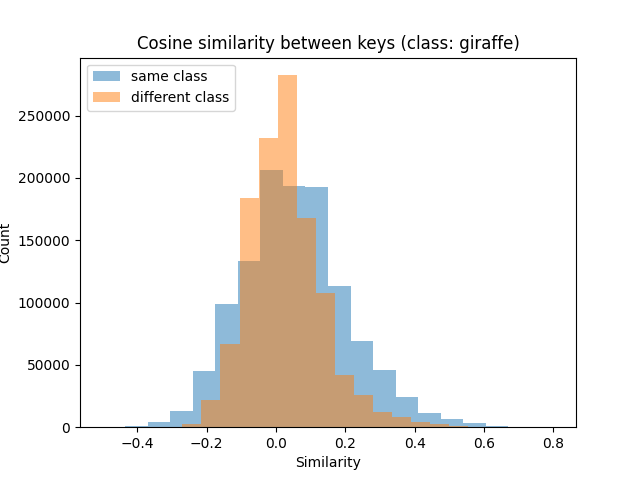
\includegraphics[width=\textwidth]{Images/same_vs_diff_class/plot_giraffe_cosine.png}
%		\caption{Cosine similarity}
%	\end{subfigure}
%	\quad
%	\begin{subfigure}[b]{0.47\textwidth}  
%		\centering 
%		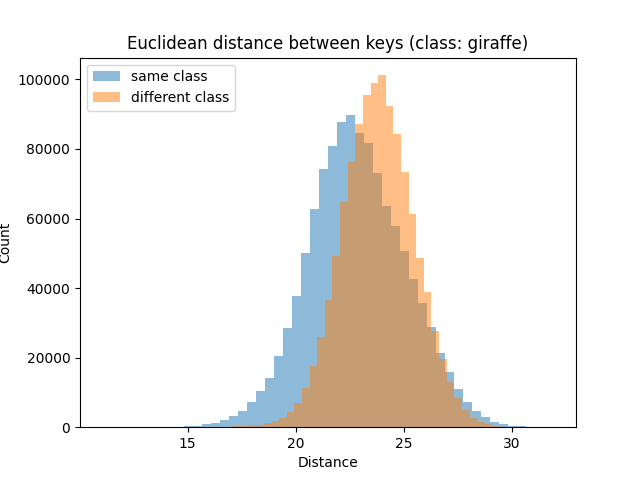
\includegraphics[width=\textwidth]{Images/same_vs_diff_class/plot_giraffe_euc.png}
%		\caption{Euclidean}
%	\end{subfigure}
%	\caption[\textbf{Comparison of keys of images of same and different classes}]{\textbf{Comparison of keys of images of same and different classes}. Shows the pattern of similarity scores and distance measure when comparing keys of same and different classes. Y axis shows number of images compared }
%	\label{fig:same_vs_diff}
%\end{figure*}
    \chapter{Experiments and Results}\label{chap:experiments}
In this chapter, we present a comprehensive analysis of the experiments conducted to compare our proposed method with the baseline approach, CutLER. We thoroughly evaluate both models across a diverse set of datasets to assess their performance. Additionally, we delve into the impact of training images containing overlapping instances, providing detailed quantitative results to illustrate how these images affect model's performance. 

\section{Datasets}
For a fair comparison, we use the same datasets as the baseline for both training and evaluation. All models are trained on the ImageNet dataset and evaluated on a diverse set of benchmark datasets, including COCO, Pascal VOC, and KITTI. This ensures more consistent and comprehensive assessment of performance across different types of datasets.

\subsection{ImageNet}
The ImageNet dataset is a large-scale visual database designed for use in visual object recognition research. Developed by researchers at Princeton and Stanford, it contains more than 10,000,000 labeled images depicting 10,000+ object categories. Each image in the dataset is hand-labeled by humans, making it a valuable resource for training and benchmarking deep learning models in computer vision.

We generate MaskCut annotations for all images on the subset of ImageNet containing the 1000 categories and 1.3 million images(ImageNet-1K), which serve as the pseudo-ground truth for our experiments. Both the baseline method (CutLER) and our proposed method are trained on the ImageNet dataset. However, in the proposed method, a fraction of images are excluded during the mask-refinement process(Images with no annotaions are removed).

\subsection{COCO}
The COCO (Common Objects in Context) dataset~\cite{lin2015microsoftcococommonobjects} is a widely-used benchmark in the field of computer vision, designed to spur advancements in object detection, segmentation, and captioning. It contains over 200,000 images with more than 80 object categories, annotated with precise bounding boxes, segmentation masks, and context-related captions. 

We use the validation set of the COCO 2017 split, which contains 5,000 images, for evaluating the models. Both bounding box coordinates and segmentation annotations are utilized as ground truths for evaluation.

\subsection{PASCAL VOC}
The PASCAL VOC 2012 dataset is a widely recognized benchmark in visual object recognition, comprising 11,530 images across 20 categories with comprehensive annotations for object detection, classification, and segmentation tasks. For evaluation, we use both the training and test images from the PASCAL VOC dataset and detailed segmentation annotations as ground truths.

\subsection{KITTI}
The KITTI dataset~\cite{Geiger2013IJRR} is a prominent benchmark for evaluating performance in autonomous driving and computer vision tasks, including object detection, tracking, and scene flow. It features high-resolution images captured from a stereo camera setup mounted on a moving vehicle, encompassing a variety of urban and rural driving scenarios. 

Although the KITTI dataset offers rich annotations, including 3D object labels and depth information, our evaluation focuses solely on bounding boxes. Since the dataset does not provide segmentation annotations, we utilize only the bounding box data to evaluate 7521 images from KITTI’s trainval split.

\subsection{Comic and Watercolor}
In addition to real-world image datasets, we also incorporate art datasets, such as Comic and Watercolor~\cite{Inoue_2018_CVPR}, to evaluate the model's generalization capabilities across diverse visual styles. Since these datasets lack segmentation annotations, we use only the bounding box data for evaluation, as in our approach for the KITTI dataset. 

\section{Implementation Details}
\label{section:implementation_details}
Our implementation largely follows the baseline approach; however, it is important to note a key difference in our setup. While in the baseline paper experiments use a batch size of 16, we utilize batch sizes of 4 and 8 due to resource constraints. To ensure a fair comparison, we also train the baseline model from scratch using these same batch sizes of 4 and 8.

\subsection{Training data}
Only the images from ImageNet dataset(1.3 Million images) are used for the training(including self-training). We do not use any supervised pretrained models or labels for training baseline or the proposed method. However, the bounding box annotations are used to analyze the impact of images with overlapping instances in section <REF:>

\subsection{MaskCut}

We apply MaskCut with N=3, generating three masks per image through repeated N-Cut operations, on images resized to 480×480 pixels to create pseudo-ground truths. The value of N is optimal at 3 for generating best quality masks for ImageNet dataset~\cite{wang2023cut}. The patch-wise affinity matrix generated from the key descriptors of the ViT-B/8 DINO model is used to perform the N-Cut operation. Additionally, we employ Conditional Random Fields (CRF) to refine the masks and extract their bounding boxes.

\subsection{Detector}
Although CutLER is designed to be agnostic to the choice of object detector, we chose to use Cascade Mask R-CNN for all our experiments. This decision is based on the baseline paper's findings, which demonstrated that Cascade Mask R-CNN outperforms Mask R-CNN. We train the detector on ImageNet with MaskCut pseudo masks and bounding boxes for 160K iterations with a batch size of 8. 

The copy-paste augmentation is also used during the training process to improve robustness of object detection and segmentation models by exposing them to a wider range of scenarios and object contexts. In order to detect small objects, instead of vanilla copy-paste augmentation, masks are randomly downsampled with a scalar uniformly sampled between 0.3 and 1.0. 

We optimize the Detector using SGD for 160K iterations with a learning rate of 0.005, weight decay of \(5×10^{−5}\) and a momentum of 0.9. Training follows a learning rate schedule which decreases it by 5 after 80K iterations.

\subsection{Self Training}
In each stage, along with CutLER mask predictions with confidence score > 0.7 generated using the model from previous stage, Maskcut masks which have IoU < 0.5 with the CutLER prediction masks together make the pseudo ground truth masks for that stage. The detector is then optimized using SGD with a learning rate of 0.01 over 80,000 iterations. We do not employ DropLoss during these self-training phases.

\subsection{Resources}
Generating MaskCut annotations for all images in ImageNet is supposed to most time consuming part. But we used the pre-generated MaskCut annotations to save time.

Initial training on ImageNet with batch size 8 spans over 160K iterations on four NVIDIA rtx-2080 gpus takes around 1 day 18 hours and self-training of 80K iteration takes around 21 hours. The Training using filtered MaskCut masks generated by our method takes 4 hours less (1 day 14 hrs) as around 130K images are dropped in the mask filtration step for not having any pseudo-ground truth masks.


\section{Experiments}
\subsection{Exploring Impact of Overlapping Instances}

\subsection{Proposed Method}

\begin{table}[htbp]
	\centering
	\begin{tabular}{c|cc|cc|cc|cc|cc}
		\toprule
		& \multicolumn{2}{c|}{COCO} & \multicolumn{2}{c|}{KITTI} & \multicolumn{2}{c|}{VOC} & \multicolumn{2}{c|}{Comic} & \multicolumn{2}{c}{Watercolor} \\ \midrule
		& AP & AP50 & AP & AP50 & AP & AP50 & AP & AP50 & AP & AP50 \\ \midrule
		\multicolumn{11}{c}{Train} \\ \midrule
		Baseline & 11.17 & 20.12 & 4.79 & 10.27 & 19.98 & 36.26 & \textbf{11.80} & \textbf{28.39} & \textbf{14.67} & \textbf{35.60} \\ \midrule
		Ours & \textbf{11.47} & \textbf{20.81} & \textbf{6.28} & \textbf{13.48} & \textbf{20.24} & \textbf{36.56} & 10.81 & 26.50 & 14.00 & 35.27 \\ \midrule
		\multicolumn{11}{c}{Self-train-r1} \\ \midrule
		Baseline & 11.70 & 21.15 & 6.60 & 14.19 & 19.56 & 36.81 &  \textbf{11.05} &  \textbf{27.53} & 12.92 & 33.45 \\ \midrule
		Ours & \textbf{11.94} & \textbf{21.65} & \textbf{8.21} & \textbf{18.49} & \textbf{20.24} & \textbf{37.95} & 10.80 & 27.40 & \textbf{15.37} & \textbf{37.74} \\
		\midrule
		\multicolumn{11}{c}{Self-train-r2} \\ \midrule
		Baseline & 11.02 & 20.32 & 6.73 & 15.02 & 18.06 & 35.09 & 9.90 & 25.36 & 13.59 & 34.31 \\ \midrule
		Ours & 11.02 & 20.32 & 6.73 & 15.02 & 18.06 & 35.09 & 9.90 & 25.36 & 13.59 & 34.31 \\ \bottomrule
	\end{tabular}
	\caption{AP and AP50 for Training and Self-Training (Batch size 8)}
	\label{tab:combined_train}
\end{table}


\begin{table}[htbp]
	\centering
	\begin{tabular}{c|c|cc|cc|cc|cc|cc}
		\toprule
		& & \multicolumn{2}{c|}{COCO} & \multicolumn{2}{c|}{KITTI} & \multicolumn{2}{c|}{VOC} & \multicolumn{2}{c|}{Comic} & \multicolumn{2}{c}{Watercolor} \\ \midrule
		& & AP & AP50 & AP & AP50 & AP & AP50 & AP & AP50 & AP & AP50 \\ \midrule
		\multirow{2}{*}{Train} & Baseline & 11.17 & 20.12 & 4.79 & 10.27 & 19.98 & 36.26 & \textbf{11.80} & \textbf{28.39} & \textbf{14.67} & \textbf{35.60} \\ 
		& Ours & \textbf{11.47} & \textbf{20.81} & \textbf{6.28} & \textbf{13.48} & \textbf{20.24} & \textbf{36.56} & 10.81 & 26.50 & 14.00 & 35.27 \\ \midrule
		\multirow{2}{*}{Self-train-r1} & Baseline & 11.70 & 21.15 & 6.60 & 14.19 & 19.56 & 36.81 & \textbf{11.05} & \textbf{27.53} & 12.92 & 33.45 \\ 
		& Ours & \textbf{11.94} & \textbf{21.65} & \textbf{8.21} & \textbf{18.49} & \textbf{20.24} & \textbf{37.95} & 10.80 & 27.40 & \textbf{15.37} & \textbf{37.74} \\ \midrule
		\multirow{2}{*}{Self-train-r2} & Baseline & 11.02 & 20.32 & 6.73 & 15.02 & 18.06 & 35.09 & 9.90 & 25.36 & 13.59 & 34.31 \\ 
		& Ours & 11.02 & 20.32 & 6.73 & 15.02 & 18.06 & 35.09 & 9.90 & 25.36 & 13.59 & 34.31 \\ \bottomrule
	\end{tabular}
	\caption{AP and AP50 for Training and Self-Training (Batch size 8)}
	\label{tab:combined_train_1}
\end{table}



\section{Result of bs-8 CutLER training}
% \todo{This section is completely adapted from openseg, add more infor and rephrase the text}

\cite{wang2023cut}
\begin{table}[htbp]
	\centering
	\begin{tabular}{c|c|c|c|c|cl}
		\toprule
		train & COCO & KITTI & VOC & Comic & Watercolor \\ \midrule
		Baseline & 11.17,20.12 & 4.79,10.27 & 19.98,36.26 & 11.80,28.39 & 14.67,35.6 \\ \midrule
		Ours & \textbf{11.47,20.81} & \textbf{6.28,13.48} & \textbf{20.24,36.56} & 10.81,26.50 & 14.00,35.27 \\ \bottomrule
	\end{tabular}
	\caption{AP and AP50}
	\label{tab:base_train}
\end{table}

\begin{table}[htbp]
	\centering
	\begin{tabular}{c|c|c|c|c|cl}
		\toprule
		self-train-r1 & COCO & KITTI & VOC & Comic & Watercolor \\ \midrule
		Baseline & 11.7,21.15 & 6.60,14.19 & 19.56,36.81 & 11.05,27.53 & 12.92,33.45 \\ \midrule
		Ours & \textbf{11.94,21.65} & \textbf{8.21,18.49} & \textbf{20.24,37.95} & 10.80,27.4 & \textbf{15.37,37.74} \\ \bottomrule
	\end{tabular}
	\caption{AP and AP50}
	\label{tab:r1_train}
\end{table}

\begin{table}[htbp]
	\centering
	\begin{tabular}{c|c|c|c|c|cl}
		\toprule
		self-train-r2 & COCO & KITTI & VOC & Comic & Watercolor \\ \midrule
		Baseline & 11.02,20.32 & 6.73,15.02 & 18.06,35.09 & 9.90,25.36 & 13.59,34.31 \\ \midrule
		Ours & - & - & - & - & - \\ \bottomrule
	\end{tabular}
	\caption{AP and AP50}
	\label{tab:r2_train}
\end{table}

\begin{table}[htbp]
	\centering
	\begin{tabular}{c|c|c|cl}
		\toprule
		Eval dataset & Imagenet-all & Imagenet-wo-ol & Imagenet-maskcut-filter \\
		\midrule
		Coco Eval & 10.35, 19.15 & 11.52, 20.67 & 11.44, 21.31 \\
		\midrule
		Coco Eval w/o overlapping inst. & 23.45, 38.11  & 24.77, 39.46 & 24.64, 40.64 \\
		\midrule
		Coco Eval only overlapping inst. & 7.25, 15.11 & 8.52, 16.8 & 8.32, 17.28 \\
		\bottomrule
	\end{tabular}
	\caption{\textbf{AP and AP50 of evaluation(box) on COCO Eval datasets on models trained on imagenet for 90K iterations}}
	\label{tab:ablationK}
\end{table}

\begin{table}[htbp]
	\centering
	\begin{tabular}{c|c|c|cl}
		\toprule
		Eval dataset & Imagenet-all & Imagenet-wo-ol & Imagenet-maskcut-filter \\
		\midrule
		Coco Eval & 7.87, 16.05 & 8.80, 17.47 & 9.1, 18.15 \\
		\midrule
		Coco Eval w/o overlapping inst. & 19.19, 35.19  & 20.13, 36.36 & 21.15, 38.31 \\
		\midrule
		Coco Eval only overlapping inst. & 5.12, 11.55 & 6.18, 13.27 & 9.78, 18.92 \\
		\bottomrule
	\end{tabular}
	\caption{\textbf{AP and AP50 of evaluation(segm) on COCO Eval datasets on models trained on imagenet for 90K iterations}}
	\label{tab:ablationK}
\end{table}

\subsection{Choice of batch size}
In the baseline paper, experiments were conducted using a batch size of 16. Due to resource constraints, we performed our experiments with batch sizes of 4 and 8. As shown in Table <Table Number>, we observe a slight improvement in performance with a higher batch size. Our experiments also indicate that batch size influences the relative improvement achieved through self-training.

For batch sizes of 4 and 8, we observed that in self-training round 2, the performance of both the baseline and our method decreased instead of improving. This contrasts with the results in the baseline paper with batch size 16, where performance continued to improve until round 2.

%\subsection{\ad}
%ADE20K, introduced by  Zhou et al., provides detailed annotations for pixel-level segmentation, covering both objects and stuff categories \cite{zhou2017scene}. The dataset is split into a training set and a validation set. The training set consists of approximately 20,000 images, while the validation set contains around 2,000 images. ADE20K is known for its comprehensive coverage of scenes and contains annotations for 150 object classes and 92 stuff categories, making it a valuable resource for zero-shot semantic segmentation in our experiments.
%
%\section{Evaluation Metric}
%\subsection{\mIoU}
%The Mean Intersection over Union (mIoU) is a widely employed evaluation metric within the field of computer vision, specifically designed for the assessment of semantic segmentation models. It quantifies the degree to which the predicted segmentation masks align with the ground truth annotations for a given semantic segmentation task involving N classes. This alignment is determined by comparing the prediction logits and ground truth logits for a specific class, denoted as `c', based on three key parameters: (i) True Positive (TP(c)): Number of pixels correctly classified as class c, (ii)False Positive (FP(c)): Number of pixels incorrectly classified as class c but should belong to other classes, (iii)
%False Negative (FN(c)): Number of pixels incorrectly classified as other classes but should belong to class c. The IoU for a specific class `c' is calculated as shown in the below Eq. \ref{eq:IoU}
%\begin{equation}
%\label{eq:IoU}
%    \text{IoU}(c) = \frac{\text{TP}(c) + \text{FP}(c) + \text{FN}(c)}{\text{TP}(c)} ,
%\end{equation}
%The final mIoU is then obtained by calculating the mean across all classes as shown in the below Eq. \ref{eq:miou} to calculate the final mIoU.
%\begin{equation}
%    \label{eq:miou}
%    mIoU = \frac{1}{N} \sum_{c=1}^{N} IoU(c),
%\end{equation}
%This metric allows researchers to effectively evaluate the performance of their semantic segmentation models and assess how well the model aligns with the ground truth
%
%
%\section{Experiment Setting}
%\label{sec:experiment}
%
%The GroupViT model is trained on a combination of CC12M and filtered YFCC datasets, amounting to a total of 26 million image-text pairs \cite{changpinyo2021conceptual, thomee2016yfcc100m}. This training spans 30 epochs and employs 16 NVIDIA V100 GPUs over a 2-day period, utilizing a batch size of 4096. The initial two epochs serve as warm-up stages, gradually increasing the learning rate from an initial value of $4 \times 10^{-6}$ to reach a base of $1.6 \times 10^{-3}$. The training process integrates a weight decay of 0.05 to counter overfitting, and gradient clipping to prevent gradient magnitudes exceeding 5.0. Employing the AdamW optimizer with epsilon set at $1 \times 10^{-8}$ and beta coefficients of 0.9 and 0.999, a cosine learning rate scheduler is employed \cite{kingma2014adam, loshchilov2016sgdr}.\\
%For our experiments, we always train the pretrained model on MSCOCO. \textit{In this context, we use `training' and `fine-tuning' interchangeably}. With a global batch size of 256, we introduce a learning rate scale of 0.01 to adjust minimum and warm-up learning rates, aiding convergence. The warm-up epoch of 1 allows gradual increase of initial learning rate. A cosine scheduler over 12 decay epochs is used, gradually reducing the learning rate with 2 cycles of annealing for refinement. If not explicitly mentioned, we use 2 NVIDIA 1080Ti GPUs for our training procedure. We use seed `123' for reproducibility if it is not explicitly mentioned.\\
%For inference, we keep an image resolution of 448, stride of 224 and crop size of 448. For background threshold, we use 0.95 for PASCAL VOC, 0.9 for COCO, 0.35 for \pcon and 0.95 for ADE20K. Note that authors of GroupViT do not evaluate on ADE20K. Therefore, we keep all settings unchanged and use the background threshold as determined by the authors of OVSegmentator \cite{xu2023learning}. We  do an ablation on these inference settings for our baseline to report the best possible setting in section \ref{sec:infsettings}
%% 
%\begin{document}
\begin{table}[htbp]
\label{tab:hp}
  \centering
  \begin{tabular}{c|c}
    \toprule
    \textbf{Hyperparameter} & \textbf{Value} \\
    \midrule
    Training Epochs & 30 \\
    \midrule
    Warmup Epochs & 0\\
    \midrule
    Batch Size & 4096 \\
    \midrule
    Learning rate(LR) scheduler &  Cosine\\
    \midrule
    Minimum LR & $4e^{-5}$ \\
    \midrule
    Warmup LR & $4e^{-6}$ \\
    \midrule
    Base LR & 0.0016\\
    \midrule
    Optimizer &  AdamW\\
    \midrule
    Weight decay & 0.05 \\
    \midrule
    Number of nouns to extract(K) & 3 \\
    \midrule
    Number of stages & 3 \\
    \midrule
    Number of transformer block on each stage & 6, 3, 3 \\
    \midrule
    Group tokens on every stage & 64, 8, 0\\
    \midrule
    Number of heads in transformer block & 6, 6, 6\\
    \midrule
    Vision Encoder embedding dimension & 384\\
    \midrule
    Number of Transformer blocks in Text encoder & 12\\
    \midrule
    Text Encoder embedding dimension & 256\\
    \midrule
    Context Length  & 77\\
    \midrule
    Vocabulary size  & 49408\\
    \midrule
    Multimodal space embedding dimension & 256\\
    \midrule
    Contrastive loss temperature  & 0.07\\
    \bottomrule
    
  \end{tabular}
  
  \caption{GroupViT  Hyperparameters}
\end{table}


%\end{document}
%% %\begin{document}
\begin{table}[htbp]
\label{tab:infhp}
  \centering
  \begin{tabular}{c|c}
    \toprule
    \textbf{Inference Hyperparameter} & \textbf{Value} \\
    \midrule
    Image resolution & 448 \\
    \midrule
    mode & slide\\
    \midrule
    stride & 224 \\
    \midrule
    crop size   & 448\\
    \midrule
    Background threshold & \pvoc(0.95) \\
                    & \pcon(0.35) \\
                    & \coco(0.9) \\
                    & \ad(0.95)\\
    \bottomrule
    
  \end{tabular}
  
  \caption{GroupViT Inference Hyperparameters}
\end{table}


%\end{document}
%
%\section{ Visual Grouping vs Visual-Text Alignment}
%\label{sec:analyse}
%In our quest to enhance the performance of the GroupViT approach and identify its limitations, we conduct a comprehensive analysis using the PASCAL VOC dataset. Within GroupViT, the Semantic Segmentation task consists of two key subtasks: visual grouping and visual-language alignment. To precisely identify GroupViT's limitations, we perform two distinct sets of experiments. In each set, we isolate and evaluate these subtasks individually.
%\subsection{Analysis of Visual Grouping}
%In the first set of experiments, we evaluate GroupViT's performance exclusively on the Visual Grouping task. We refrain from using GroupViT's labeling mechanism and instead propose an alternative approach, as explained below.
%
%\subsubsection{Feature Extraction}
%We extract features using the pretrained GroupViT model for the training split of the Pascal VOC 2012 dataset. Images are processed through the visual encoder with frozen weights, where they are grouped into 8 segments in the final stage. We use features from the final stage, denoted as ${\hat{S}_i^{3}}$, to build a feature bank represented as $\mathbb{F} \in \mathbb{R}^{|\hat{S}^3| \times D}$. In our setup, $D$ represents the visual encoder's dimension, which is 384, and $|\hat{S}^3|$ represents the number of segment tokens obtained after the final stage, which is 8. This configuration results in 8 features per image. For our experiment, the feature bank contains a total of 11,592 features.
%
%\subsubsection{Soft Label Assignment}
%To label the features, we deviate from GroupViT's label assignment method. Similar to the inference process outlined in Section \ref{sec:inf}, we compute the global soft attention of group tokens, denoted as $\text{\textbf{Attn}} \in \mathbb{R}^{|G^2| \times |S^1|}$, as shown in Eq. \ref{eq:globalsoftattn}. The attention map is then reshaped into a $|G^2| \times P \times P$ format, where $P \times P$ corresponds to a $16 \times 16$ patch token format. We use bilinear interpolation to resize the map to $G^2 \times H \times W$, where $H$ and $W$ represent the image's height and width. By performing an argmax operation, we assign pixels to specific groups, resulting in a 2D vector of size $H \times W$ that indicates group associations, as demonstrated in Eq. \ref{eq:argmaxsecondlevelgrouping}. This process yields a segmented image.
%
%% \begin{equation}
%% \label{eq:secondlevelgrouping}
%%     \hat{X} = 
%% \end{equation}
%\begin{equation}
%\label{eq:argmaxsecondlevelgrouping}
%    \text{Segmented\_Image} = \text{Argmax}(\text{Interpolate}(\textbf{Attn}))
%\end{equation}
%To label the segments in the obtained segmented image, we extract their corresponding labels from the ground truth mask, denoted as M. To address cases where some pixels of a feature are labeled as class `A' while others are labeled as class `B,' we implement a soft label assignment approach. This method captures varying degrees of association, offering a more flexible representation of visual content.
%
%To achieve this, we maintain a soft label vector $S \in \mathbb{R}^{|\hat{S}^3| \times (N+1)}$, where $|\hat{S}^3|$ is the number of segments, and $N+1$ represents the class count, including the background class. For instance, in the case of Pascal VOC 2012 with 21 classes, each image feature is associated with a 21-sized array, where the indices correspond to class assignments. If all the pixels of a feature  belong to class `A', the corresponding index is set to 1. When out of N pixels, X pixels belong to class `A' and (N-X) pixels belong to class `B', the indices for class `A' and class `B' would have values X/N and (N-X)/N, respectively. Each index ideally represents the percentage of segment area associated with a specific class.
%
%\subsubsection{Find K-Nearest Neighbors (KNN)} 
%After obtaining soft labels for the features, our goal is to train a K-Nearest Neighbors (KNN) model \cite{cover1967nearest}. To ensure balanced features, we set a maximum limit of 1000 features for each category. We also conducted ablation experiments on the value of K, as shown in Table \ref{tab:ablationK}, and present the results in Table \ref{tab:analyssiresult}.
%
%\subsubsection{Evaluation}
%To evaluate the validation set, we follow the same procedure as for the training set to extract group token features. Let $V$ be the set of images in the validation set. For each image $v \in V$, we extract features of its segment tokens $F_v = {f_{v1}, f_{v2}, \ldots, f_{v8}}$, where $f_{vi}$ represents the $i$th segment token feature of image $v$.
%
%Next, we find the nearest neighbors for each feature in the validation set. We use $T$ to denote the bag of features obtained from the training set. For each segment token feature $f_{vi}$ of an image $v$, we find its $k$ nearest neighbors $KNN_{vi} = {t_{vi1}, t_{vi2}, \ldots, t_{vik}}$ from $T$. We aggregate their corresponding soft labels $S_{vik}$ using the mean operation:
%
%\begin{equation}
%\label{eq:analysisaggre}
%\overline{S_{vi}} = \frac{1}{k} \sum_{t_{vik} \in {KNN}{vi}} S_{vik}
%\end{equation}
%
%We then apply the argmax operation to the aggregated soft labels $\overline{S_{vi}}$ to obtain the final label $y_{vi}$ for each segment token feature $f_{vi}$:
%
%\begin{equation}
%\label{eq:labelassign}
%y_{vi} = \arg\max(\overline{S_{vi}})
%\end{equation}
%
%This process provides us with the final labels for all segment token features in the validation set. Using these labels, we obtain the segmentation logits and evaluate the segmentation results using the mean Intersection over Union (mIoU) metric. The results are presented in Table \ref{tab:analyssiresult}.
%
%In summary, the procedure entails the extraction of segment token features from the final stage for the training split of the PASCAL VOC dataset to create a bag of features. We fit a KNN model on these features. We then extract the features for the validation split. Nearest neighbors are identified for all the features, and soft labels are aggregated, allowing for the assignment of final labels. We then obtain segmentation logits, and evaluate the mIoU score on the dataset. This holistic process offers valuable insights into the model's performance in terms of visual grouping.
%
%
%\subsection{Analysis of Vision-Text Alignment}
% 
%We analyze the performance of the Vision-Text alignment mechanism of \gvit on \pvoc without utilizing visual grouping, relying solely on ground truth masks. Following the inference pipeline in Section \ref{sec:inf}, we compute the metric $\textbf{L}_{affinity} \in \mathbb{R}^{ H \times W \times N }$ as defined in Eq. \ref{eq:pred}, where H and W represent the image's height and width, respectively, and N is the number of classes.
%
%Next, we load the ground truth mask for an image, where each pixel is labeled with its associated class, including the background. Let $M$ be the ground truth mask, with each entry $M_{i,j}$ representing the class label at pixel $(i,j)$. For each class $c$ in $M$, we gather all pixels belonging to class $c$ in $\textbf{L}_{affinity}$ to identify groups in $\textbf{L}_{affinity}$ without employing \gvit's grouping mechanism. Specifically, all pixels associated with class `c' form a group, denoted as $G_c$. We calculate the mean of this group of pixels, $M_{G_c}$, along the last dimension (representing classes) to obtain a mean channel value for all pixels in the group. We then perform an argmax operation over the class channel to obtain $C_{G_c}$, as shown in Eq. \ref{eq:assignment}. Here, $C_{G_c}$ refers to the class assigned to all pixels in group $G_c$:
%
%\begin{equation}
%\label{eq:mean}
%M_{G_c} = \frac{1}{|G_c|} \sum_{p=1}^{|G_c|} \textbf{L}_{affinity}(p)
%\end{equation}
%
%\begin{equation}
%\label{eq:assignment}
%C_{G_c} = \text{Argmax}( M_{G_c})
%\end{equation}
%% \begin{equation}
%% \label{eq:variance}
%% V_{G_c} = \frac{1}{|G_c|} \sum_{p=1}^{|G_c|} (\textbf{L}_{\text{affinity}}(p) - M_{G_c})^2
%% \end{equation}
%
%We then label all associated pixels with the obtained class $C_{G_c}$. This way, we identify groups by grouping all pixels belonging to the same class based on the ground truth mask, without using the grouping mechanism of \gvit. We assign class labels using the GroupViT mechanism, and the results are presented in Table \ref{tab:analyssiresult}. 
%We note that while Visual Grouping and Visual-Text alignment both outperform GroupViT individually, it is evident that Visual Grouping exhibits a larger potential for improvement compared to alignment. We also conducted an evaluation without the background class to report the mIoU score, eliminating the reliance on the susceptibility of the background threshold.
%
%% Additionally, we calculate the variance, $V_{G_c}$, as shown in Eq. \ref{eq:variance}, to measure the variance of Intersection over Union (IoU) for different categories. We observe higher variance for categories like `person' `monitor' and `table' compared to others. This variance is likely due to visual differences caused by varying orientations and appearances. For example, `monitor' may have different displays in different images, contributing to higher visual variance. `Person' may share the scene with various complementary objects, leading to increased variance.
%\begin{figure*}
%
%  %   \begin{tabular}{ccccc}
%  %   \textbf{Image} & \textbf{Column 2} & \textbf{Column 3} & \textbf{Column 4} &    \textbf{Ground Truth}\\
%  % \end{tabular}
%  \centering
%   % \rotatebox{45}{\textbf{\footnotesize  Image}}\hfill
%   % \rotatebox{45}{\textbf{\footnotesize Visual-Text alignment}}\hfill
%   % \rotatebox{45}{\textbf{\footnotesize Visual Grouping}}\hfill
%   % \rotatebox{45}{\textbf{\footnotesize GroupViT}}\hfill
%   % \rotatebox{45}{\textbf{\footnotesize Ground-Truth}}
%  % \subfloat {\textbf{\footnotesize Image}}
%  % \hfill
%  % \subfloat {\textbf{\footnotesize  \ \ \ \ \ \ Visual-Text}}
%  % \hfill
%  % \subfloat {\textbf{\footnotesize Visual}}
%  % \hfill
%  % \subfloat {\textbf{\footnotesize GroupViT}}
%  % \hfill
%  % \subfloat {\textbf{\footnotesize Ground-Truth}}
%  
%  % \vspace{-0.1em}
%  
%  % \subfloat {\textbf{}}
%  % \hfill
%  % \subfloat {\textbf{\footnotesize \ Alignment}}
%  % %\hfill
%  % \subfloat {\textbf{\footnotesize \ \ \ \ \ \ \ \ \ Grouping}}
%  % \hfill
%  % \subfloat {\textbf{}}
%  % \hfill
%  % \subfloat {\textbf{\footnotesize }}
%
%  % \vspace{-0.1em}
%  \subfloat {\textbf{\small \ \ Image}}
%  \hspace{4em}
%  \subfloat {\textbf{\small Alignment}}
%  \hspace{1.5em}
%  \subfloat {\textbf{\small Grouping}}
%  \hspace{1.5em}
%  \subfloat {\textbf{\small \ \ \ \ GroupViT}}
%  \hspace{2em}
%  \subfloat {\textbf{\small Ground-Truth}}
%  
%  \vspace{-0.02em} 
%  \vspace{-0.05em} 
%  %  \subfloat {\textbf{\small \ \ Image}}
%  % \hspace{4em}
%  % \subfloat {\textbf{\small \ \ \ Alignment}}
%  % \hspace{1.5em}
%  % \subfloat {\textbf{\small Grouping}}
%  % \hspace{1.5em}
%  % \subfloat {\textbf{\small GroupViT}}
%  % \hspace{1.5em}
%  % \subfloat {\textbf{\small \ \ \ \ Ground-Truth}}
%  % \vspace{-0.02em} 
%  % \vspace{-0.05em}
%  
%  {\includegraphics[width=0.19\textwidth]{Images/analysis/0000.jpg}}
%  {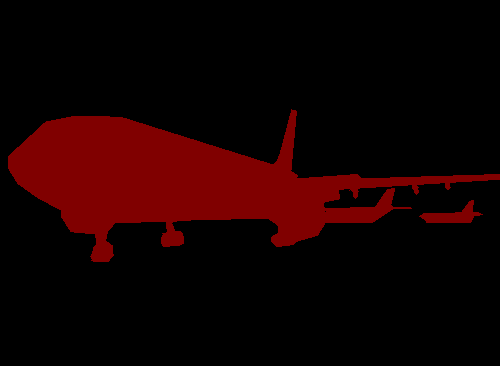
\includegraphics[width=0.19\textwidth]{Images/analysis/0.png}}
%  {
\includegraphics[width=0.19\textwidth]{Images/analysis/colored_mask_gi_val0.png}}
%  {
\includegraphics[width=0.19\textwidth]{Images/analysis/originalcheckpoint/0000.png}}
%  {
\includegraphics[width=0.19\textwidth]{Images/analysis/2007_000033.png}}
%  {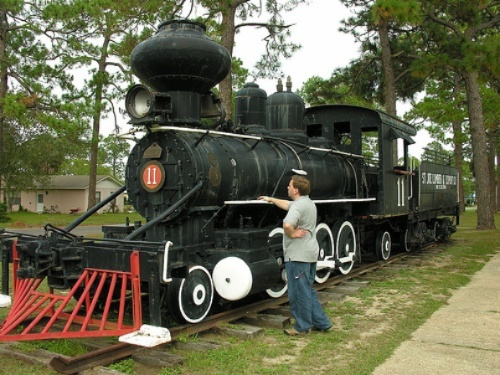
\includegraphics[width=0.19\textwidth]{Images/analysis/0081.jpg}}
%  {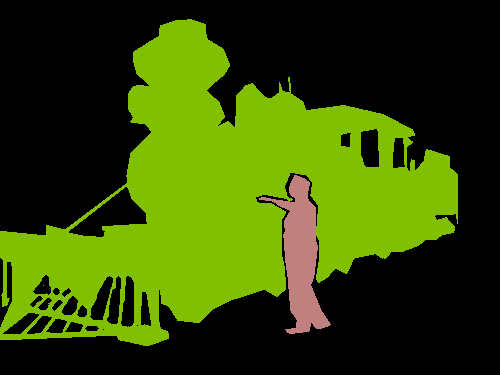
\includegraphics[width=0.19\textwidth]{Images/analysis/81.png}}
%  {
\includegraphics[width=0.19\textwidth]{Images/analysis/colored_mask_gi_val81.png}}
%  {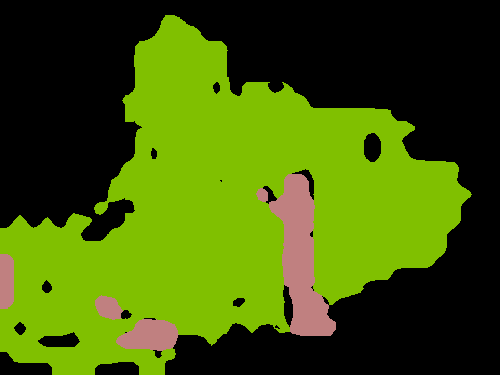
\includegraphics[width=0.19\textwidth]{Images/analysis/originalcheckpoint/0081.png}}
%  {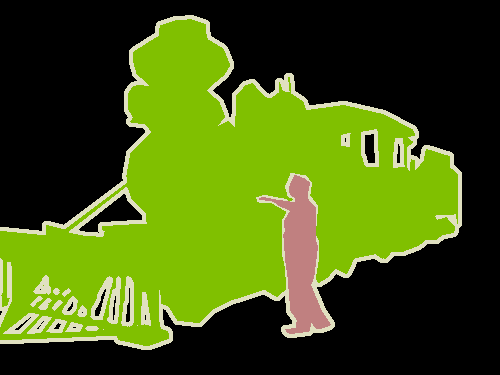
\includegraphics[width=0.19\textwidth]{Images/analysis/2007_002565.png}}
%  {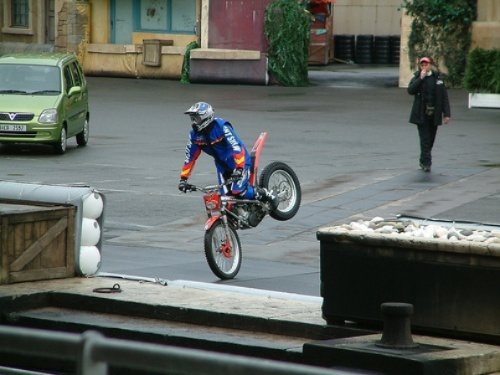
\includegraphics[width=0.19\textwidth]{Images/analysis/0086.jpg}}
%  {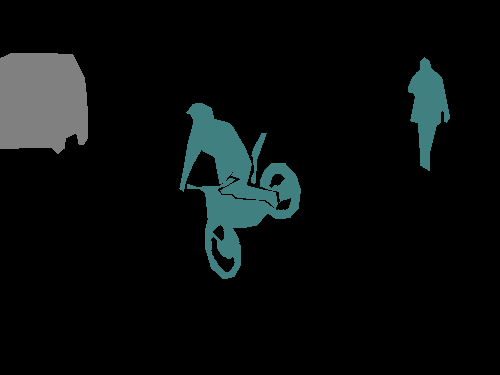
\includegraphics[width=0.19\textwidth]{Images/analysis/86.png}}
%  {
\includegraphics[width=0.19\textwidth]{Images/analysis/colored_mask_gi_val86.png}}
%  {
\includegraphics[width=0.19\textwidth]{Images/analysis/originalcheckpoint/0086.png}}
%  {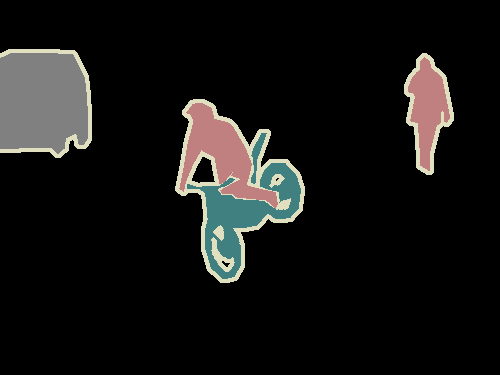
\includegraphics[width=0.19\textwidth]{Images/analysis/2007_002643.png}}
%  {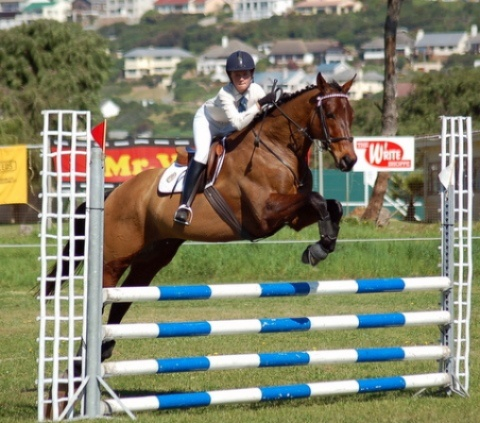
\includegraphics[width=0.19\textwidth]{Images/analysis/0262.jpg}}
%  {
\includegraphics[width=0.19\textwidth]{Images/analysis/262.png}}
%  {
\includegraphics[width=0.19\textwidth]{Images/analysis/colored_mask_gi_val262.png}}
%  {
\includegraphics[width=0.19\textwidth]{Images/analysis/originalcheckpoint/0262.png}}
%  {
\includegraphics[width=0.19\textwidth]{Images/analysis/2007_008256.png}}
%  {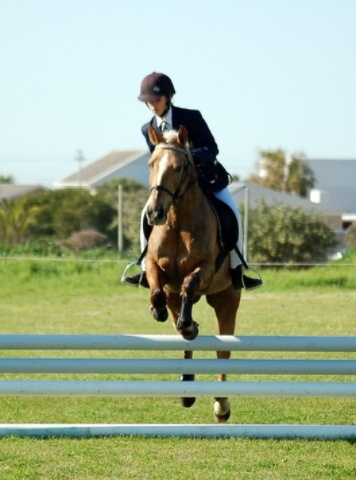
\includegraphics[width=0.19\textwidth]{Images/analysis/0270.jpg}}
%  {
\includegraphics[width=0.19\textwidth]{Images/analysis/270.png}}
%  {
\includegraphics[width=0.19\textwidth]{Images/analysis/colored_mask_gi_val270.png}}
%{
\includegraphics[width=0.19\textwidth]{Images/analysis/originalcheckpoint/0270.png}}
%  {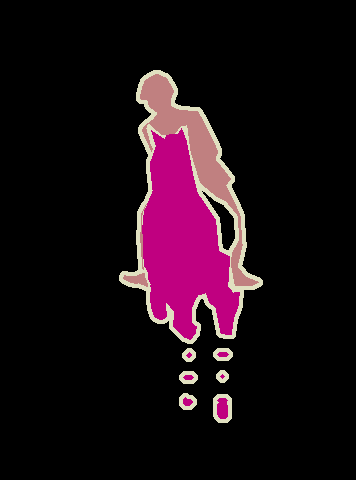
\includegraphics[width=0.19\textwidth]{Images/analysis/2007_008596.png}}
%\caption[\textbf{Visualization of Visual Grouping Vs Visual-Text Alignment}]{\textbf{Visualization of Visual Grouping Vs Visual-Text Alignment}. Comparison of Segmentation Masks using Different Models. The first and last columns show image and the corresponding ground truth segmentation masks, while the remaining columns display the segmentation masks generated by Visual-Text alignment, Visual grouping and the Original checkpoint.}
%    
%\end{figure*}
%
%
% \begin{table}[htbp]
% \begin{center}
%     \begin{tabular}{|c|c|c|}
%         \hline
%         Model &  Data & mIoU     \\ \hline
%         \gvit & \pvoc & $52.29$  \\
%         \gvit & \coco & $24.3$   \\
%         \ovs  & \pvoc & $53.78$  \\
%         \ovs  & \coco & $25.06$  \\
%         \hline
%     \end{tabular}
%     \end{center}

%     \caption[Table caption]{\textbf{Table caption.} foo bar...\\}
%     \label{tab:accuracy}
% \end{table}



\begin{table}[htbp]
  \centering
  
  \begin{tabular}{c|c|cl}
    \toprule
    Model & Type & \pvoc \\
    \midrule
    \gvit & Original & 52.29  \\
    \midrule
    \gvit & Visual Grouping  & 54.16  \\
    \midrule
    \gvit & Visual Grouping(WB)  & 56.12  \\
    \midrule
    \gvit & Visual-Text Alignment & \textbf{76.18}  \\
    \bottomrule
  \end{tabular}
  \caption[\textbf{Analysis of Visual Grouping and Visual-Text Alignment}]{\textbf{Analysis of Individual Components.} Here, `Visual Grouping (WB)' refers to the evaluation performed without considering the `background' class.}
  
 \label{tab:analyssiresult}
\end{table}


\begin{table}[htbp]
  \centering
  \begin{tabular}{c|c|cl}
    \toprule
    Model & K & \pvoc \\
    \midrule
    Visual Grouping & 5 & 51.85 \\
    \midrule
    Visual Grouping & 10  & 54.26  \\
    \midrule
    Visual Grouping & 15 & 51.93  \\
    \midrule
    Visual Grouping & 25 & 49.66  \\
    \bottomrule
  \end{tabular}
  \caption{\textbf{Ablation on number of nearest neighbors for Visual Grouping}}
 \label{tab:ablationK}
\end{table}


% \documentclass{article}
% \usepackage{booktabs}

% \begin{document}

% \begin{table}[htbp]
%   \centering
%   \caption{My Pretty Table}
%   \begin{tabular}{ccc}
%     \toprule
%     Column 1 & Column 2 & Column 3 \\
%     \midrule
%     Row 1, Cell 1 & Row 1, Cell 2 & Row 1, Cell 3 \\
%     Row 2, Cell 1 & Row 2, Cell 2 & Row 2, Cell 3 \\
%     Row 3, Cell 1 & Row 3, Cell 2 & Row 3, Cell 3 \\
%     \bottomrule
%   \end{tabular}
% \end{table}

% \end{document}
%
%% \todo{add observation, variation across each class, ablation over k, with and without background}
%
%
%\section{Fine-tuning the Pretrained Model}
%In the previous section, our feature analysis highlighted opportunities to enhance GroupViT's visual grouping capabilities. These insights have motivated us to explore its full potential further. However, GroupViT is a substantial model with 55 million parameters, trained on a large dataset. Starting training from scratch would be resource-intensive. Instead, we've chosen to fine-tune the pretrained model, leveraging the valuable knowledge it acquired during its initial training phase and its understanding of visual and linguistic concepts. This approach also helps accelerate convergence. Our fine-tuning process involves training on a smaller and cleaner dataset, MSCOCO. This dataset provides human-annotated captions, which are believed to offer richer information about the corresponding images compared to the web-scaled datasets used in pretraining.
%
%\subsection{Choice of Components}
%To comprehensively analyze the core components of GroupViT for segmentation, we propose fine-tuning the Grouping Blocks and MLP Projectors. This aims to improve visual grouping quality and alignment in an image-text pair. We systematically evaluate different combinations within the visual encoder and report results in Table \ref{tab:ft}. 
%The experiment was conducted over 15 epochs.
%We observe that tuning both Grouping Blocks results in better performance compared to the other combinations. This validates our earlier findings in Section \ref{sec:analyse}, where we identified a greater room for improvement in visual grouping.
%
%\begin{document}
\begin{table}[htbp]
  \centering
  \begin{tabular}{c|c|c|l|l|l}
    \toprule
    \multirow{2}{*}{Model} & Fine-tuned & \multicolumn{4}{c}{Datasets} \\
    %\cmidrule(lr){1-2} \cmidrule(lr){3-4}
    \cline{3-6}
    & components & COCO & PVOC & PContext & ADE20K \\
    \midrule
    \gvit & Original & 24.3  & \textbf{52.29} & 22.39 &  \textbf{8.59}\\
    \midrule
    \gvit & Both GBs & \textbf{26.15}  & 49.18 & 21.87 & 7.50 \\
    \midrule
    \gvit & 2nd GB & 25.79 & 49.15 & 21.71 & 7.69 \\
    \midrule
    \gvit & Both GBs  & 25.62 & 49.22 & \textbf{22.41} & 8.49\\
          & + Img Proj &  &  &  & \\
    \midrule
    \gvit & 2nd GB  & 25.79 & 50.90 & 22.33 & 8.25\\
     &  + Img Proj &  &  &  & \\ 
    \midrule
    \gvit & Both GBs +  & 25.05 & 48.33 & 22.39 & 7.61\\
    
     &  Projs &  &  &  & \\
    \midrule
    \gvit & 2nd GB + Projs &  25.04 & 47.94 & 21.7 & 7.67\\
    \midrule
    \gvit & Img Proj & 24.48 & 50.32 & 22.36 & 8.27\\
    % \midrule
    % \gvit & VE &  & & & \\
    \midrule
    \gvit & Projs & 24.49 & 50.24 & 21.87 & 8.15\\
    \bottomrule
    
  \end{tabular}
  
  \caption[\textbf{Choice of Architectural Components to Fine-tune}]{\textbf{Choice of Architectural Components to Fine-tune}. Here, `GBs' stands for Grouping Blocks, while `Img Proj' represents the Image Projector within the Visual Encoder. `Projs' refers to both the Text MLP Projector and the Image MLP Projector. `+' is used to represent a combination of components.}
  
\label{tab:ft}
\end{table}


%\end{document}

% \begin{table}[t]
%     \scriptsize
%     \centering
%     \caption{Assessment of Approaches}
%     \label{tab:multi_shape}
%     \setlength\tabcolsep{5.0pt}
%     \begin{threeparttable}
%         \begin{tabular}{c|c|c|c|c|c|c|c|c}
%             \toprule
%                 \multirow{2}{2.0cm}{GroupViT} &  \multirow{2}{.5cm}{\centering GB1} & \multirow{2}{.5cm}{\centering GB2} &\multirow{2}{.5cm}{\centering IP} 
%                 &\multirow{2}{.5cm}{\centering TP} & \multicolumn{4}{c}{Datasets} \\
%                 %\cmidrule(lr){1-2} \cmidrule(lr){3-4}        
%                 \cline{6-9}
%                 & &  &  & & COCO & PVOC & PContext & ADE20K \\

%                 \midrule
%                 %single shape + sum & 65 & 70 & 68 \\
%                  Original & - & - & - & - & 24.3  & \textbf{52.29} & 22.39 &  \textbf{8.59} \\
%                 \midrule
%                  %Img Proj
%                 \multirow{10}{*}{Fine-tuned} & - & - & - & \checkmark & 24.48 & 50.32 & 22.36 & 8.27 \\
%                 \cmidrule{2-9}
%                 %Text Proj
%                  & - & - & \checkmark & \checkmark & 24.49 & 50.24 & 21.87 & 8.15 \\
%                 \cmidrule{2-9}
%                 %2ndGB
%                  & - & \checkmark & - & - & 25.79 & 49.15 & 21.71 & 7.69  \\
%                 \cmidrule{2-9}
%                 %2ndGB + Img Proj
%                  & - & \checkmark & \checkmark & - & 25.79 & 50.90 & 22.33 & 8.25 \\
%                 \cmidrule{2-9}
%                 %2ndGB + Img Proj + Text Proj
%                 & - & \checkmark & \checkmark & \checkmark & 25.04 & 47.94 & 21.7 & 7.67 \\
%                 \cmidrule{2-9}
%                 %BothGBs
%                  & \checkmark & \checkmark & - & - &  \textbf{26.15}  & 49.18 & 21.87 & 7.50 \\
%                 \cmidrule{2-9}
%                 %BothGBs +ImgProj
%                  & \checkmark & \checkmark & \checkmark & - & 25.62 & 49.22 & \textbf{22.41} & 8.49 \\
%                 \cmidrule{2-9}
%                  %BothGBs +ImgProj + TextProj
%                  & \checkmark & \checkmark & \checkmark & \checkmark & 25.05 & 48.33 & 22.39 & 7.61 \\
                
%                 \bottomrule
%         \end{tabular}
%     \footnotesize
%     \vspace{.3em}
%     \hspace{-.11\linewidth}

%     \end{threeparttable}
%     \vspace{-0.3cm}
% \end{table}


% \begin{table}[t]
%     \scriptsize
%     \centering
%     \caption{}
%     \label{tab:multi_shape}
%     \setlength\tabcolsep{5.0pt}
%     \begin{threeparttable}
%         \begin{tabular}{c|c|c|c|c|c|c|c|c}
%             \toprule
%                 GroupViT &   GB1 & GB2 & IP & TP & COCO \\
%                 %\cmidrule(lr){1-2} \cmidrule(lr){3-4}        


%                 \midrule
%                 %single shape + sum & 65 & 70 & 68 \\
%                  Original & - & - & - & - & 24.3  & \textbf{52.29} & 22.39 &  \textbf{8.59} \\
%                 \midrule
%                  %Img Proj
%                 \multirow{10}{*}{Fine-tuned} & - & - & - & \checkmark & 24.48 & 50.32 & 22.36 & 8.27 \\
%                 \cmidrule{2-9}
%                 %Text Proj
%                  & - & - & \checkmark & \checkmark & 24.49 & 50.24 & 21.87 & 8.15 \\
%                 \cmidrule{2-9}
%                 %2ndGB
%                  & - & \checkmark & - & - & 25.79 & 49.15 & 21.71 & 7.69  \\
%                 \cmidrule{2-9}
%                 %2ndGB + Img Proj
%                  & - & \checkmark & \checkmark & - & 25.79 & 50.90 & 22.33 & 8.25 \\
%                 \cmidrule{2-9}
%                 %2ndGB + Img Proj + Text Proj
%                 & - & \checkmark & \checkmark & \checkmark & 25.04 & 47.94 & 21.7 & 7.67 \\
%                 \cmidrule{2-9}
%                 %BothGBs
%                  & \checkmark & \checkmark & - & - &  \textbf{26.15}  & 49.18 & 21.87 & 7.50 \\
%                 \cmidrule{2-9}
%                 %BothGBs +ImgProj
%                  & \checkmark & \checkmark & \checkmark & - & 25.62 & 49.22 & \textbf{22.41} & 8.49 \\
%                 \cmidrule{2-9}
%                  %BothGBs +ImgProj + TextProj
%                  & \checkmark & \checkmark & \checkmark & \checkmark & 25.05 & 48.33 & 22.39 & 7.61 \\
                
%                 \bottomrule
%         \end{tabular}
%     \footnotesize
%     \vspace{.3em}
%     \hspace{-.11\linewidth}

%     \end{threeparttable}
%     \vspace{-0.3cm}
% \end{table}
%\subsection{Choice of Batch Size}
%In our experiments, we change the global batch size to three different values: 256, 512, and 1024 and train the model for 10 epochs. In Table \ref{tab:batchsize}, we observe improved performance with a batch size of 1024 on \pvoc and PASCAL Context, while a batch size of 512 works best on COCO, as detailed in Table \ref{tab:batchsize}. While the literature suggests that a larger pool of negative samples can enhance contrastive loss outcomes \cite{jia2021scaling}\cite{radford2021learning}, it's also noted that large data scales are needed to counteract the impact of noisy image-text training \cite{jia2021scaling}. Our hypothesis aligns with our specific context: training on a relatively smaller yet cleaner dataset. This suggests that the noise introduced during training is not sufficiently mitigated, making a relatively smaller batch size of 512 a more effective choice. 
%% \begin{table}[htbp]
%   \centering

%   \begin{tabular}{ccc}
%     \toprule
%     Model & Batch Size & MSCOCO \\
%     \midrule
%     \gvit & 256 & \textbf{26.49} \\
%     \gvit & 512 & 26.4 \\
%     \gvit & 1024 & 26.16 \\
%     \bottomrule
%   \end{tabular}
%   \caption[\textbf{Choice of Batch Size}]{\textbf{Choice of Batch Size }}
%  \label{tab:batchsize}
% \end{table}

\begin{table}[htbp]
  \centering
  \begin{tabular}{c|c|c|l|l|l}
    \toprule
     \multirow{2}{*}{Model} & \multirow{2}{*}{Batch Size} & \multicolumn{4}{c}{Datasets} \\
    %\cmidrule(lr){1-2} \cmidrule(lr){3-4}
    \cline{3-6}
    &  & COCO & PVOC & PContext & ADE20K \\
    \midrule
    \gvit & 256 & 25.96 & 48.67 & 21.64 & 7.60\\
    %\gvit & VE& 45.46 & 21.44 \\
    \midrule
    
    \gvit & 512 & \textbf{26.13}   & 49.29 & 21.63 & \textbf{7.92}\\
    \midrule
    
    \gvit & 1024 & 25.92  & \textbf{49.73} & \textbf{21.71} & 7.57\\
    %\ovs  & GB + MMD & 53.78 & 25.06 \\
    \bottomrule
  \end{tabular}
  \caption[\textbf{Choice of Batch Size}]{\textbf{Choice of Batch Size }}
  \label{tab:batchsize}
\end{table}


%Due to resource constraints and only marginal differences in model performance across different batch sizes, we choose to proceed with a batch size of 256 for our experiments. However, as we observe some improvement with a batch size of 512, we will report the performance of our baseline, obtained later in Section \ref{sec:nncl}, using a global batch size of 512.
%
%
%\section{Exploring Impact of Multi-label}
%\label{sec:explabel}
%We investigate how extracted nouns affect performance, particularly their impact on embedding context. To enhance context, we extract comprehensive noun phrases from captions using NLTK and a regex expression. These phrases include adjectives before nouns and are denoted as `NP' in Table \ref{tab:texthierarchy}. Furthermore, we experiment with varying the number of extracted nouns and phrases (3, 5, 7 labels) to assess their effect on performance.
%
%In addition, we train a model without multi-label contrastive loss, and the results are shown in Table \ref{tab:texthierarchy}. Notably, we observe that the model trained on Noun Phrases, Nouns, and captions, with an upper limit of 5 on extracted labels, outperforms other settings. However, intriguingly, we observe similar performance for the model trained solely with contrastive loss and the one trained with both multi-label contrastive loss and contrastive loss.
%
%To provide a more robust analysis, we conduct experiments on 3 different seeds (0, 100, 200) for `NP+Nouns+Captions with 5 labels' and `Caption'. The results are summarized as mean and variance mIoU in Table \ref{tab:texthierarchy}. Visualizations in Figure \ref{fig:plot_text} confirmed convergence to similar performance, with slight initial speed-ups for multi-label training.
%
%As a result, we decide to proceed with the `NP+Nouns+Caption' model with 5 labels for subsequent experiments. This choice aligns with Xu et al.'s findings during GroupViT training \cite{xu2022groupvit}.
%
%
%

% \begin{table}[htbp]
% \begin{center}
%     \begin{tabular}{|c|c|c|}
%         \hline
%         Model &  Data & mIoU     \\ \hline
%         \gvit & \pvoc & $52.29$  \\
%         \gvit & \coco & $24.3$   \\
%         \ovs  & \pvoc & $53.78$  \\
%         \ovs  & \coco & $25.06$  \\
%         \hline
%     \end{tabular}
%     \end{center}

%     \caption[Table caption]{\textbf{Table caption.} foo bar...\\}
%     \label{tab:accuracy}
% \end{table}

% \begin{table}[htbp]
%   \centering
%   \caption{GroupViT - Ablation on Text hierarchy}
%   \begin{tabular}{cccc|l}
%     \toprule
%     Model & #labels & Text-Type & \multicolumn{2}{c}{Datasets} \\
%     \cmidrule(lr){1-3} \cmidrule(lr){4-5}
%     & &&\pvoc & \coco \\
%     \midrule
%     \gvit & 3 & Nouns+Caption & 49.65 & 26.32 \\
%     \gvit & 3 & NounPhrases+Noun+Caption & 50.24 & 26.35 \\
%     \gvit & 5 & NounPhrases+Noun+Caption & 50.16 & 26.5 \\
%     \gvit & 0 & Caption &  & 26.35 \\
%     \bottomrule
%   \end{tabular}
% \end{table}

% \begin{table}[htbp]
%   \centering
%   \begin{tabular}{ccc|c|l}
%     \toprule
%     Model & \#labels & Text-Type & \multicolumn{2}{c}{Datasets} \\
%     \cmidrule(lr){1-4} \cmidrule(lr){4-5}
%     & & & COCO & VOC\\
%     \midrule
%     \gvit & 3 & Nouns+Caption  & 26.32 & 49.65\\
%     \gvit & 3 & NP+Nouns+Caption & 26.35 & 50.24 \\
%     \gvit & 5 & NP+Nouns+Caption & \textbf{$26.74 \pm 0.0462$} & \textbf{$49.80 \pm 0.0042$}\\
%     \gvit & 7 & NP+Nouns+Caption  & 25.67 & 48.11 \\
%     \gvit & 0 & Caption  & $26.61 \pm 0.0175$ & \textbf{$51.79 \pm 0.0769$} \\
%     \bottomrule
%   \end{tabular}
%     \caption[\textbf{Exploring impact of Text hierarchy}]{\textbf{Exploring impact of Text hierarchy.}The model "NP+Nouns+Caption" extracts noun phrases and nouns for use in multi-label contrastive loss and captions for contrastive loss. While the model "Nouns+Caption" extracts just noun for use in multi-label contrastive loss. The model "Caption" is trained without multi-label contrastive loss  }
    
%   \label{tab:texthierarchy}
% \end{table}
% \begin{table}[htbp]
%   \centering
%   \begin{tabular}{c|c|c|c|llll}
%     \toprule
%     \multirow{2}{*}{Model} & \multirow{2}{*}{\#labels} &\multirow{2}{*}{Text-Type}& \multicolumn{2}{c}{Datasets} \\
%     \cline{4-7}
%       % \cmidrule(lr){4-5}
%     & & & COCO & VOC & Context & ADE20K\\
%     \midrule
%     \gvit & 3 & Nouns+Caption  & 26.32 & 49.65 & 22.04 & 7.95\\
%     \gvit & 3 & NP+Nouns+Caption & 26.35 & 50.24 & 22.09 & 8.17\\
%     \gvit & 5 & NP+Nouns+Caption & \textbf{26.74 $\pm$ 0.0462} & 49.80 $\pm$ 0.0042 & 21.92 $\pm$ 0.0061 & \\
%     \gvit & 7 & NP+Nouns+Caption  & 25.67 & 48.11 & 21.78 & 7.66 \\
%     \gvit & 0 & Caption  & 26.61 $\pm$ 0.0175 & \textbf{51.79 $\pm$ 0.0769} & 21.83 $\pm$ 0.0049 & \\
%     \bottomrule
%   \end{tabular}
%   \caption[\textbf{Exploring the Impact of Text Hierarchy}]{\textbf{Exploring the Impact of Text Hierarchy.} The model `NP+Nouns+Caption' extracts noun phrases and nouns for use in multi-label contrastive loss and captions for contrastive loss, while the model `Nouns+Caption' extracts only nouns for use in multi-label contrastive loss. The model `Caption' is trained without multi-label contrastive loss.}
%   \label{tab:texthierarchy}
% \end{table}
% \begin{table}[htbp]
%   \centering
%   \begin{tabular}{c|c|c|c|llll}
%     \toprule
%     \multirow{2}{*}{Model} & \multirow{2}{*}{\#labels} &\multirow{2}{*}{Text-Type}& \multicolumn{2}{c}{Datasets} \\
%     \cline{4-7}
%       % \cmidrule(lr){4-5}
%     & & & COCO & VOC & Context & ADE20K\\
%     \midrule
%     \gvit & 3 & Nouns+Caption  & 26.32 & 49.65 & 22.04 & 7.95\\
%     \gvit & 3 & NP+Nouns+Caption & 26.35 & 50.24 & 22.09 & 8.17\\
%     \gvit & 5 & NP+Nouns+Caption & \textbf{26.74 $\pm$ 0.0462} & 49.80 $\pm$ 0.0042 & 21.92 $\pm$ 0.0061 & \\
%     \gvit & 7 & NP+Nouns+Caption  & 25.67 & 48.11 & 21.78 & 7.66 \\
%     \gvit & 0 & Caption  & 26.61 $\pm$ 0.0175 & \textbf{51.79 $\pm$ 0.0769} & 21.83 $\pm$ 0.0049 & \\
%     \bottomrule
%   \end{tabular}
%   \caption[\textbf{Exploring the Impact of Text Hierarchy}]{\textbf{Exploring the Impact of Text Hierarchy.} The model `NP+Nouns+Caption' extracts noun phrases and nouns for use in multi-label contrastive loss and captions for contrastive loss, while the model `Nouns+Caption' extracts only nouns for use in multi-label contrastive loss. The model `Caption' is trained without multi-label contrastive loss.}
%   \label{tab:texthierarchy}
% \end{table}


\begin{table}[htbp]
  \centering
  \small % Reduce font size
  \setlength{\tabcolsep}{3.5pt} % Reduce column padding
  \begin{tabular}{c|c|c|c|c|c|c}
    \toprule
    \multirow{2}{*}{Model} & \multirow{2}{*}{\#labels} & \multirow{2}{*}{Type} & \multicolumn{4}{c}{Datasets} \\
    \cline{4-7}
    & & & COCO & PVOC & PContext & ADE20K\\
    \midrule
     \gvit(Original) & 3 & Nouns+caption &  24.3 & \textbf{52.29}  & \textbf{22.39} & \textbf{8.56}\\
     \midrule
    \multirow{2}{*}{\gvit} & \multirow{2}{*}{3} & Nouns & \multirow{2}{*}{26.32} & \multirow{2}{*}{49.65} & \multirow{2}{*}{22.04} & \multirow{2}{*}{7.95}\\
    & & +Caption& & & & \\
    \midrule
    \multirow{2}{*}{\gvit} & \multirow{2}{*}{3} & NP+Nouns & \multirow{2}{*}{26.35} & \multirow{2}{*}{50.24} & \multirow{2}{*}{\textbf{22.09}} & \multirow{2}{*}{\textbf{8.17}}\\
    & &+Caption & & & & \\
    \midrule
    \multirow{2}{*}{\gvit} & \multirow{2}{*}{5} & NP+Nouns & \textbf{26.74} & 49.80  & 21.92 & 7.42\\
    
    & & + Caption & \textbf{$\pm$ 0.0462} & $\pm$ 0.0042 & $\pm$ 0.0061 & $\pm$ 0.0022\\
   \midrule
    \multirow{2}{*}{\gvit} & \multirow{2}{*}{7} & NP+Nouns & \multirow{2}{*}{25.67} & \multirow{2}{*}{48.11} & \multirow{2}{*}{21.78} & \multirow{2}{*}{7.66} \\
    & & +Caption & & & & \\
   \midrule
    \multirow{2}{*}{\gvit} & \multirow{2}{*}{0} & \multirow{2}{*}{Caption} & 26.61 & 51.79 & 21.83  & 7.45 \\
    
    & & & $\pm$ 0.0175 & $\pm$ 0.0769 & $\pm$ 0.0049 & $\pm$ 0.0104\\
    
    \bottomrule
  \end{tabular}
  \caption[\textbf{Exploring the Impact of Text Hierarchy}]{\textbf{Exploring the Impact of Text Hierarchy.} The model `NP+Nouns+Caption' extracts noun phrases and nouns for use in multi-label contrastive loss and captions for contrastive loss, while the model `Nouns+Caption' extracts only nouns for use in multi-label contrastive loss. The model `Caption' is trained without multi-label contrastive loss.}
  \label{tab:texthierarchy}
\end{table}



% \begin{table}[t]
%     \scriptsize
%     \centering
%     \caption{Assessment of Approaches}
%     \label{tab:multi_shape}
%     \setlength\tabcolsep{5.0pt}
%     \begin{threeparttable}
%         \begin{tabular}{c|c|c|c|c|c|c|c|c}
%             \toprule
%                 % \multirow{2}{2.0cm}{GroupViT} &  \multirow{2}{1.5cm}{\centering Nouns} &\multirow{2}{1.5cm}{\centering Noun Phrases}&\multirow{2}{1.5cm}{\centering Caption} & \multirow{2}{1.5cm}{\centering \#Extracted Texts} &\multicolumn{4}{c}{Datasets} \\
%                 % %\cmidrule(lr){1-2} \cmidrule(lr){3-4}        
%                 % \cline{6-9}
%                 % & &  &  & & COCO & PVOC & PContext & ADE20K \\
%                 %\toprule
%                 GroupViT &  Noun & Noun Phrases & Caption & \#Extracted Texts & COCO \\
%                 %\cmidrule(lr){1-2} \cmidrule(lr){3-4}        


%                 \midrule
%                 %single shape + sum & 65 & 70 & 68 \\
%                  Original & \checkmark & - & \checkmark & 3 & 24.3  & \textbf{52.29} & \textbf{22.39} &  \textbf{8.59} \\
%                 \midrule
%                 \multirow{8}{*}{\centering Fine-tuned} & \checkmark & - & \checkmark& 3  & 26.32 & 49.65 & 22.04 & 7.95 \\
%                 \cmidrule{2-9}
%                 %GE
%                  & \multirow{4}{*}{\checkmark} & \multirow{4}{*}{\checkmark}  & \multirow{4}{*}{\checkmark}  & 3 & 26.35 & 50.24 & 22.09 & 8.17 \\
%                  %LE
%                  \cmidrule{5-9}
%                  &  &   & & 5 & \textbf{26.74} & 49.80  & 21.92 & 7.42\\
    
%     % & &  & &&\textbf{$\pm$ 0.0462} & $\pm$ 0.0042 & $\pm$ 0.0061 & $\pm$ 0.0022\\
%                 %SE
%                 \cmidrule{5-9}
%                  &  &  &  & 7 & 25.67 & 48.11 & 21.78 & 7.66 \\
%                 %\midrule
%                 %GE+LE
%                 \cmidrule{2-9}
%                  & - & - & \checkmark & 0 & 26.61 & 51.79 & 21.83  & 7.45 \\
%                % & & & && $\pm$ 0.0175 & $\pm$ 0.0769 & $\pm$ 0.0049 & $\pm$ 0.0104\\
             
%                 \bottomrule
%         \end{tabular}
%     \footnotesize
%     \vspace{.3em}
%     \hspace{-.11\linewidth}

%     \end{threeparttable}
%     \vspace{-0.3cm}
% \end{table}

% \begin{table}[htbp]
%   \centering
%   \caption{GroupViT - Impact of curated labels }
%   \begin{tabular}{ccc|l}
%     \toprule
%     Model & Method & \multicolumn{2}{c}{Datasets} \\
%     \cmidrule(lr){1-2} \cmidrule(lr){3-4}
%     & &\coco & \pvoc \\
%     \midrule
%     \gvit & All entities & 25.76 \\
%     \gvit & Entity\_freq$>=1K$ & 25.63 \\
%     \gvit & Entity\_freq$>=5K$ & 24.83 \\
%     \bottomrule
%   \end{tabular}
% \end{table}



%%\begin{figure}[t]
\begin{centering}
   
    {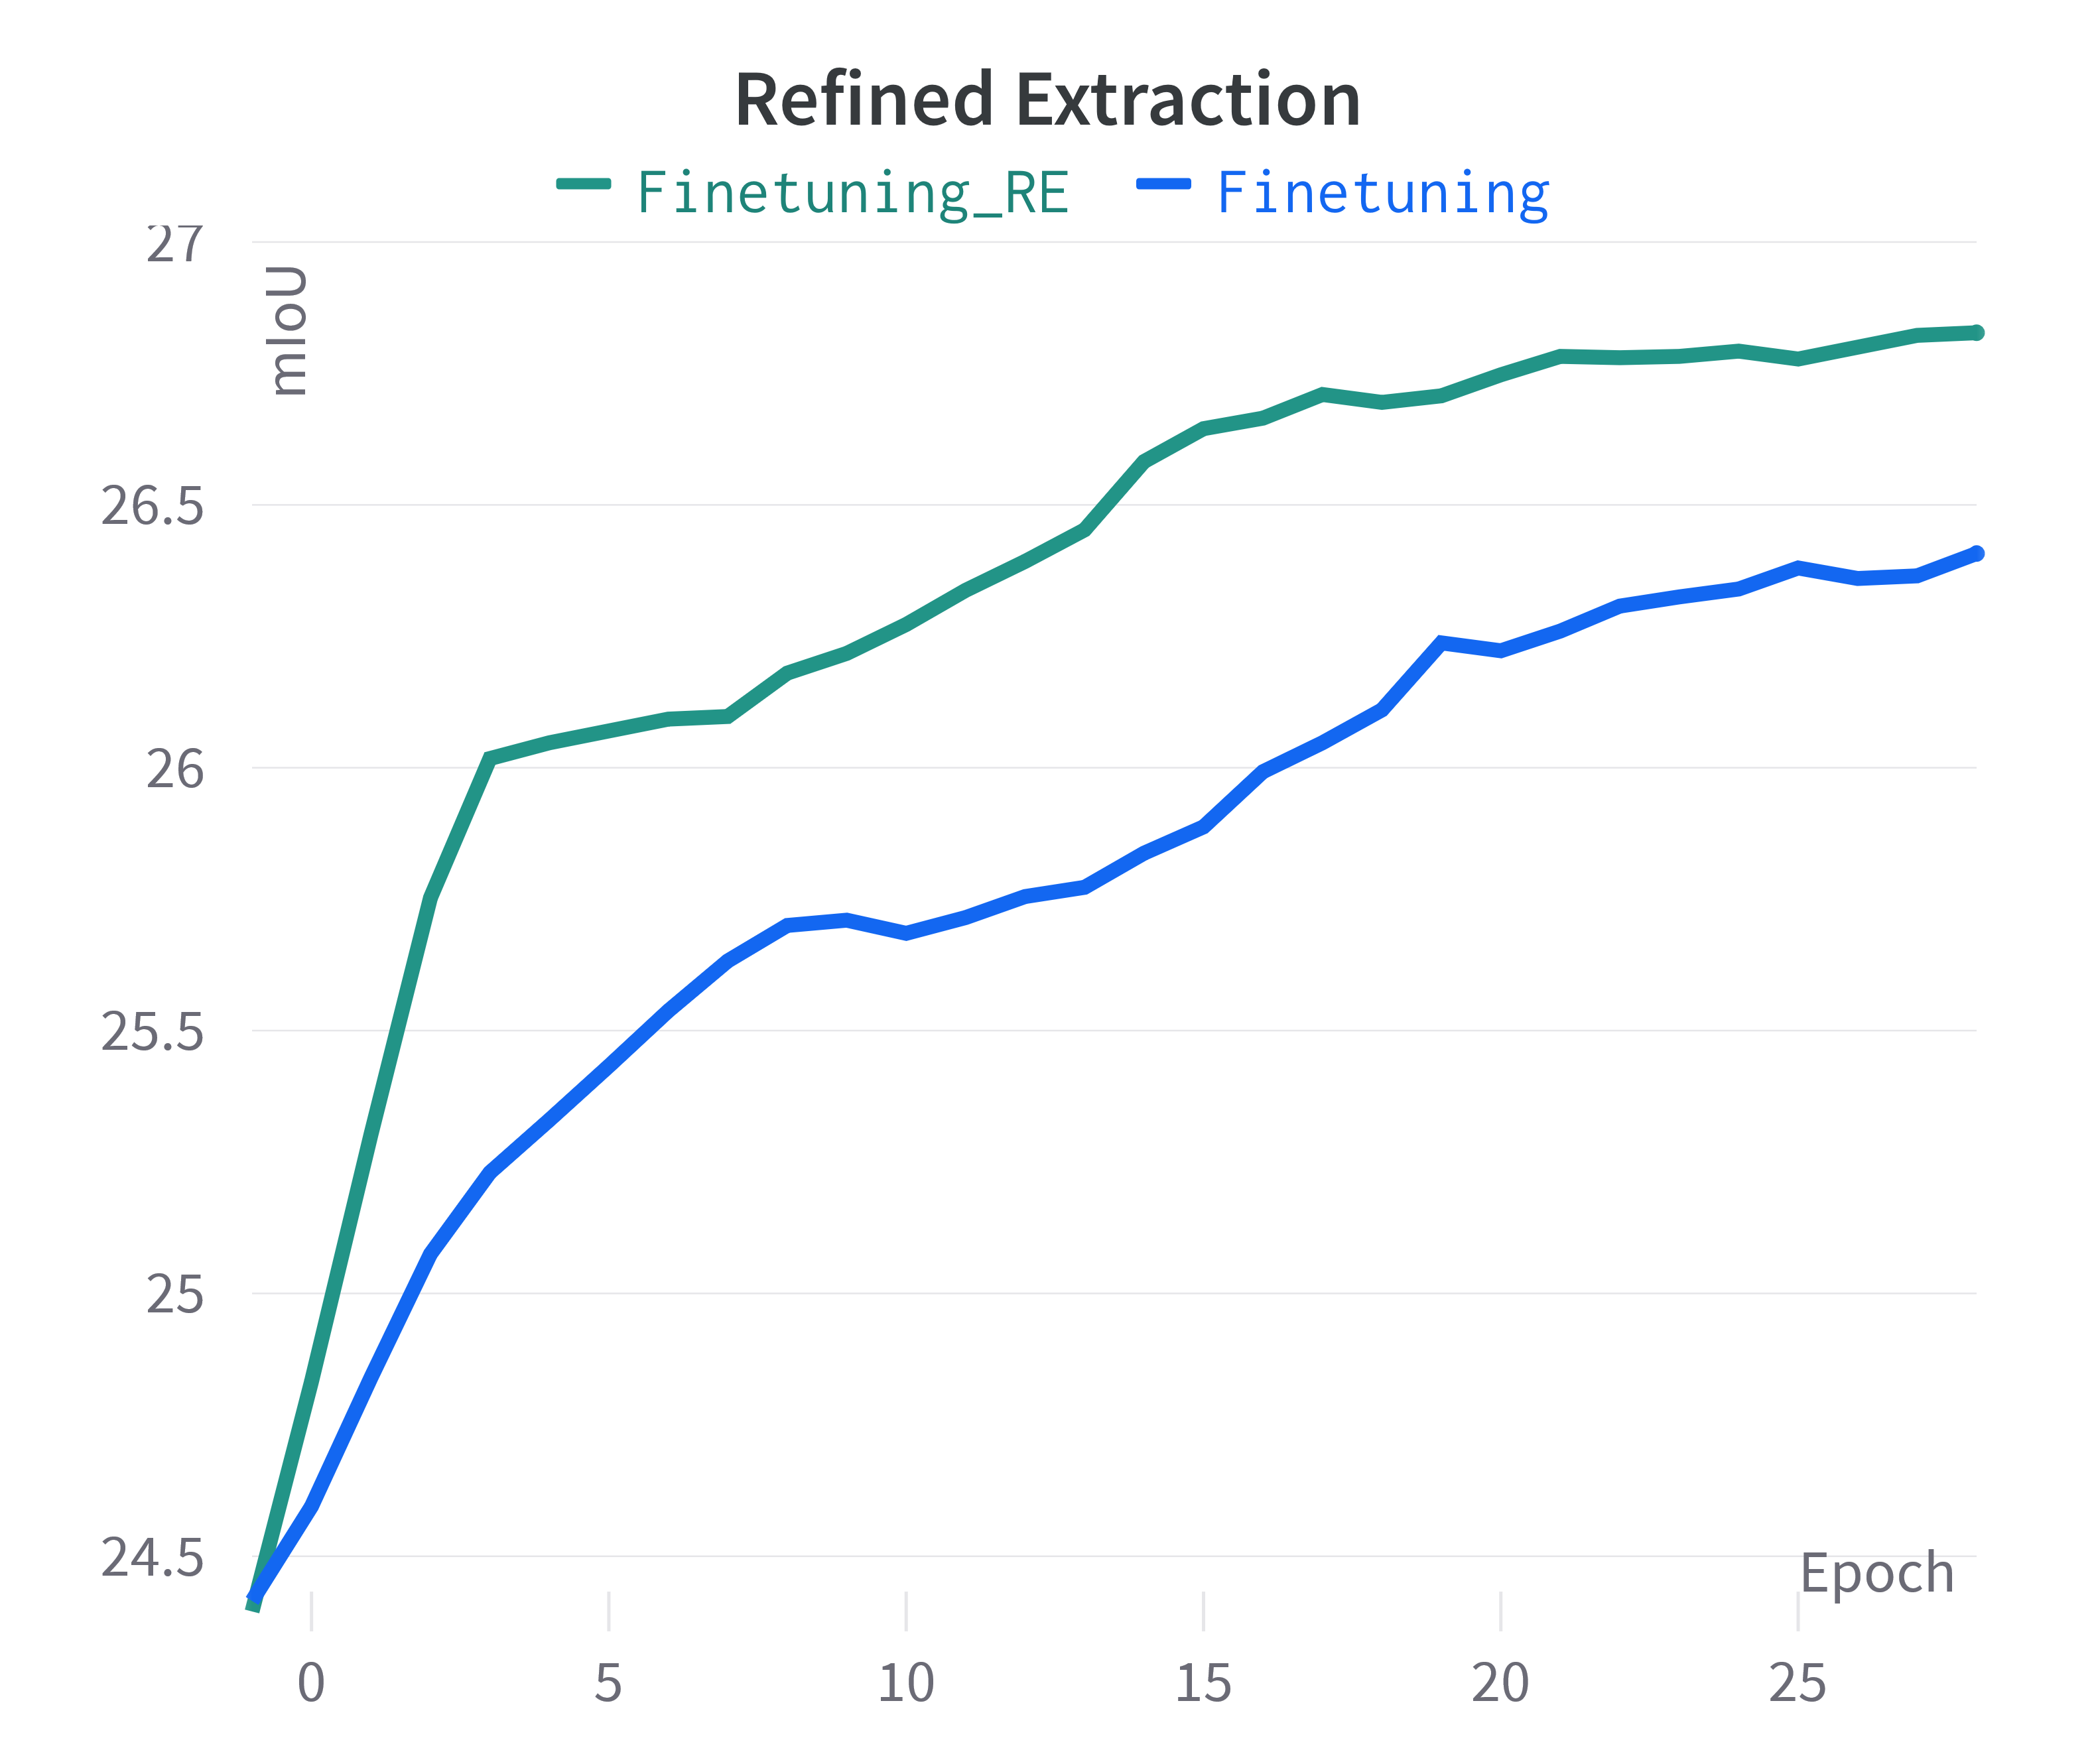
\includegraphics[scale=0.13]{figures/experiments/plots/refinedextraction.png}}
    \caption[Refined Text Extraction]{}
    % \caption[Ablation Study on Number of Stages]{\textbf{Ablation Study on Number of Stages}}
    \label{fig:pcaclasses}
\end{centering}
\end{figure}
%\section{Refinement in Label Extraction}
%\label{sec:ftre}
%For multi-label loss, GroupViT extracts a defined number of nouns or noun phrases from the caption. However, when the number of extracted labels fall short of this defined count, we address this by duplicating the caption. This ensures that the required number of labels is reached, maintaining consistent input lengths across all instances. To enhance clarity and reduce noise, we propose to substitute the caption with the <PAD> token. As <PAD> tokens are primarily introduced to ensure uniform input length, their embeddings are devoid of meaningful content. Therefore, we suggest assigning null values to their embeddings, encouraging the model to focus exclusively on pertinent input information and minimizing bias introduced by padding tokens. Our experiments, spanning over 30 epochs, reveals an improvement in performance, as indicated in Table \ref{tab:refinedextraction}. This discovery motivates us to adopt the practice of embedding <PAD> tokens with void embeddings. We provide a qualitative analysis of this baseline on PASCAL VOC in Fig. \ref{fig:qualitative_refined}
%% \begin{table}[htbp]
% \begin{center}
%     \begin{tabular}{|c|c|c|}
%         \hline
%         Model &  Data & mIoU     \\ \hline
%         \gvit & \pvoc & $52.29$  \\
%         \gvit & \coco & $24.3$   \\
%         \ovs  & \pvoc & $53.78$  \\
%         \ovs  & \coco & $25.06$  \\
%         \hline
%     \end{tabular}
%     \end{center}

%     \caption[Table caption]{\textbf{Table caption.} foo bar...\\}
%     \label{tab:accuracy}
% \end{table}




% \begin{table}[htbp]
%   \centering
%   \caption{GroupViT vs OVSegmentator}
%   \begin{tabular}{ccc|l|l|l}
%     \toprule
%     Model & Finetuned & \multicolumn{4}{c}{Datasets} \\
%     %\cmidrule(lr){1-2} \cmidrule(lr){3-4}
%     & components& VOC & COCO & ADE20K & Context\\
%     \midrule
%     \gvit(Original) &  & 52.29 & 24.3 \\
%     \gvit & GB  & 50.16 & 26.26 \\
%     \gvit & VE & 45.46 & 21.44 \\
%     \gvit(NPE) & GB & 50.45 & 26.78 \\
%     \ovs  & GB + MMD & 53.78 & 25.06 \\
%     \bottomrule
%   \end{tabular}
% \end{table}



\begin{table}[htbp]
  \centering
  \begin{tabular}{c|c|c|l|l|l}
    \toprule
    \multirow{2}{*}{Model} & \multirow{2}{*}{Method} & \multicolumn{4}{c}{Datasets} \\
    %\cmidrule(lr){1-2} \cmidrule(lr){3-4}
    \cline{3-6}
    &  & COCO & PVOC & PContext & ADE20K \\
     
    \midrule
    \gvit & Original & 24.3 & 52.29  & 22.39 & 8.56\\
    \midrule
    \gvit & Fine-tuning & 25.64  & 48.26 & 21.33 & \textbf{7.64}\\
    %\gvit & VE& 45.46 & 21.44 \\
    \midrule
    \gvit & \textbf{Fine-tuning} & \textbf{26.2} & \textbf{49.37} & \textbf{21.88} & 7.61 \\
      & \textbf{with refined extraction} &  &  && \\
    %\ovs  & GB + MMD & 53.78 & 25.06 \\
    \bottomrule
  \end{tabular}
  \caption[\textbf{Fine-tuning with Refined Extraction of Labels}]{\textbf{Fine-tuning with Refined Extraction of Labels.} We compare vanilla fine-tuning with the model trained with refined label extraction methodology. We also provide mIoU score of the pretrained model for reference.}
  \label{tab:refinedextraction}
\end{table}

\begin{table}[htbp]
  \centering
  \begin{tabular}{c|c|c|l|l|l}
    \toprule
    \multirow{2}{*}{Model} & \multirow{2}{*}{Method} & \multicolumn{4}{c}{Datasets} \\
    %\cmidrule(lr){1-2} \cmidrule(lr){3-4}
    \cline{3-6}
    &  & COCO & PVOC & PContext & ADE20K \\
     
    \midrule
    \multirow{4}{*}{\gvit} & {\color{gray}Original} & {\color{gray}24.3} & {\color{gray}52.29}  & {\color{gray}22.39} & {\color{gray}8.56}\\
    \cmidrule{2-6}
     & Fine-tuning & 25.64  & 48.26 & 21.33 & \textbf{7.64}\\
    %\gvit & VE& 45.46 & 21.44 \\
    \cmidrule{2-6}
     & Fine-tuning & \textbf{26.2} & \textbf{49.37} & \textbf{21.88} & 7.61 \\
      & with Refined Text Set &  &  && \\
    %\ovs  & GB + MMD & 53.78 & 25.06 \\
    \bottomrule
  \end{tabular}
  \caption[\textbf{Fine-tuning with Refined Extraction of Labels}]{\textbf{Fine-tuning with Refined Extraction of Labels.} We compare vanilla fine-tuning with the model trained with refined label extraction methodology. We also provide mIoU score of the pretrained model for reference.}
  \label{tab:refinedextraction}
\end{table}




% \begin{table}[htbp]
%   \centering
%   \caption{GroupViT - Impact of curated labels }
%   \begin{tabular}{ccc|l}
%     \toprule
%     Model & Method & \multicolumn{2}{c}{Datasets} \\
%     \cmidrule(lr){1-2} \cmidrule(lr){3-4}
%     & &\coco & \pvoc \\
%     \midrule
%     \gvit & All entities & 25.76 \\
%     \gvit & Entity\_freq$>=1K$ & 25.63 \\
%     \gvit & Entity\_freq$>=5K$ & 24.83 \\
%     \bottomrule
%   \end{tabular}
% \end{table}


% \documentclass{article}
% \usepackage{booktabs}

% \begin{document}

% \begin{table}[htbp]
%   \centering
%   \caption{My Pretty Table}
%   \begin{tabular}{ccc}
%     \toprule
%     Column 1 & Column 2 & Column 3 \\
%     \midrule
%     Row 1, Cell 1 & Row 1, Cell 2 & Row 1, Cell 3 \\
%     Row 2, Cell 1 & Row 2, Cell 2 & Row 2, Cell 3 \\
%     Row 3, Cell 1 & Row 3, Cell 2 & Row 3, Cell 3 \\
%     \bottomrule
%   \end{tabular}
% \end{table}

% \end{document}
%
%\begin{figure}[t]
%  %   \begin{tabular}{ccccc}
%  %   \textbf{Image} & \textbf{Column 2} & \textbf{Column 3} & \textbf{Column 4} &    \textbf{Ground Truth}\\
%  % \end{tabular}
%  \centering
%
%  \vspace{-0.5em}
% 
%  \subfloat {\textbf{\small \ \ Image}}
%  \hspace{4em}
%  \subfloat {\textbf{\small \ \ \ \ \ \ Pretrained}}
%  \hspace{4em}
%  \subfloat {\textbf{\small \ \ Fine-tuned}}
%  \hspace{2em}
%  \subfloat {\textbf{\small \ \ Ground-Truth}}
%  \vspace{-0.05em} 
%  \vspace{-0.05em} 
%  {\includegraphics[width=0.24\textwidth]{figures/experiments/pascal/0000.jpg}}
%  {
\includegraphics[width=0.24\textwidth]{figures/experiments/pascal/orgckpt/0000.png}}
%  {
\includegraphics[width=0.24\textwidth]{figures/experiments/pascal/ft/0000.png}}
%  {
\includegraphics[width=0.24\textwidth]{figures/experiments/pascal/gt/2007_000033.png}}
%  
%  {\includegraphics[width=0.24\textwidth]{figures/experiments/pascal/0010.jpg}}
%  {\includegraphics[width=0.24\textwidth]{figures/experiments/pascal/orgckpt/0010.png}}
%  {\includegraphics[width=0.24\textwidth]{figures/experiments/pascal/ft/0010.png}}
%  {\includegraphics[width=0.24\textwidth]{figures/experiments/pascal/gt/2007_000452.png}}
%  
%  {\includegraphics[width=0.24\textwidth]{figures/experiments/pascal/0013.jpg}}
%  {\includegraphics[width=0.24\textwidth]{figures/experiments/pascal/orgckpt/0013.png}}
%  {\includegraphics[width=0.24\textwidth]{figures/experiments/pascal/ft/0013.png}}
%  {\includegraphics[width=0.24\textwidth]{figures/experiments/pascal/gt/2007_000529.png}}
%
%  {\includegraphics[width=0.24\textwidth]{figures/experiments/pascal/image/0039.jpg}}
%  {\includegraphics[width=0.24\textwidth]{figures/experiments/pascal/orgckpt/0039.png}}
%  {\includegraphics[width=0.24\textwidth]{figures/experiments/pascal/ft/0039.png}}
%  {\includegraphics[width=0.24\textwidth]{figures/experiments/pascal/gt/2007_001311.png}}
%\caption[\textbf{Qualitative Analysis after Fine-tuning on Pascal VOC}]{\textbf{Qualitative Analysis after Fine-tuning GroupViT on Pascal VOC}}
%\label{fig:qualitative_refined}
%
%\end{figure}
%
%
%\subsection{Extract Labels with Most Frequent Entities}
%
%In our text augmentation process, detailed in Section \ref{sec:text_aug}, we extract nouns from caption using NLTK. It is often observed that NLTK  misidentifies nouns and extracts words like `twice', `exact', `Jonas', `TYPING', etc., despite our focus on Nouns (`NN'), Plural Nouns (`NNS'), and Proper Nouns (`NNP'). It is important to note that NLTK tags such as `NN', `NNS', and `NNP' serve as the basis for GroupViT's noun extraction from captions.\\
%For our next set of experiments, we extract all nouns and their frequencies from the MSCOCO training dataset, resulting in 27,089 nouns. We observe that a substantial number of these nouns lacked clear entity representation. To address this, we choose two sets: one with nouns appearing more than 1000 times (383 nouns) in the entire training dataset, and another with frequencies exceeding 5000 (88 nouns). Our intention was to create cleaner label sets that would offer a more precise entity representation.\\
%During training, we extract nouns and retain those belonging to the selected noun sets. If the count of retained nouns fall below the desired number of labels, we resort to using other nouns extracted from captions using the NLTK library, following the standard procedure. \\
%Intriguingly, we observe that the model exhibits better performance with the conventional extraction method. Our speculation revolves around the idea that selecting nouns based on their frequency might overly focus the model on a narrow selection of entities, hampering its ability to learn other entities or their synonyms.\\
%The results of our experiments utilizing the curated set of nouns with frequencies exceeding 1000 and 5000 were shown in Table \ref{tab:curatedlabels}. However, since we do not observe significant performance improvements and witness less promising performance during the initial epochs, we restrict the model training to the initial 5 epochs.
%% \begin{table}[htbp]
%   \centering

%   \begin{tabular}{ccc}
%     \toprule
%     Model & Method & COCO \\
%     \midrule
%     \gvit & All entities & 25.76 \\
%     \gvit & Entity\_freq$>=1K$ & 25.25 \\
%     \gvit & Entity\_freq$>=5K$ & 23.86 \\
%     \bottomrule
%   \end{tabular}
%   \caption[\textbf{Impact of curated labels}]{\textbf{Impact of curated labels }}
%  \label{tab:curatedlabels}
% \end{table}
\begin{table}[htbp]
  \centering
  \begin{tabular}{c|c|c|l|l|l}
    \toprule
    \multirow{2}{*}{Model} & \multirow{2}{*}{Method} & \multicolumn{4}{c}{Datasets} \\
    %\cmidrule(lr){1-2} \cmidrule(lr){3-4}
    \cline{3-6}
    &  & COCO & PVOC & PContext & ADE20K \\
    \midrule
    \gvit & All Entities & \textbf{25.76} & \textbf{49.20} & \textbf{21.87} & \textbf{7.50}\\
    %\gvit & VE& 45.46 & 21.44 \\
    \midrule
    
    \gvit &  Entity\_freq$>=1K$ & 25.25   & 48.70 & 21.72 & 6.95\\
    \midrule
    
    \gvit &  Entity\_freq$>=5K$ & 23.86  & 46.87 & 21.19 & 6.63\\
    %\ovs  & GB + MMD & 53.78 & 25.06 \\
    \bottomrule
  \end{tabular}
   \caption[\textbf{Impact of Curated Labels}]
   {\textbf{Impact of Curated Labels.} We assess the impact of curated labels by comparing the mIoU scores of three models: one trained with labels having frequencies over 1K in the COCO Caption dataset (`Entity\_freq$\geq1$K'), another with labels having frequencies over 5K (`Entity\_freq$\geq5$K'), and the vanilla model, which includes all entities.}
   % {Here, we compare mIoU score of model trained with labels with high frequencies in the training dataset with the vanilla model. Model ` Entity\_freq$>=1K$' prioritise labels having frequency over 1K in the COCO Caption dataset while extracting labels from caption.  Model ` Entity\_freq$>=5K$' prioritise labels having frequency over 5K. Model 'All Entities' is the vanilla mdoel }
 \label{tab:curatedlabels}
\end{table}
%\begin{figure}[t]
%\centering
%\begin{subfigure}{0.3\textwidth}
%    \centering
%    \includegraphics[width=\linewidth]{figures/experiments/entropymaps/finetuned/13/0013.jpg}
%\end{subfigure}
%\begin{subfigure}{0.3\textwidth}
%    \centering
%    \includegraphics[width=\linewidth]{figures/experiments/entropymaps/finetuned/13/entropy_mapwithoutcb.png}
%\end{subfigure}
%\begin{subfigure}{0.3\textwidth}
%\label{fig:postregentropy}
%    \centering
%    \includegraphics[width=\linewidth]{figures/experiments/entropymaps/er/13/entropy_mapwithoutcb.png}
%\end{subfigure}
%\begin{subfigure}{0.3\textwidth}
%    \centering
%    \includegraphics[width=\linewidth]{figures/experiments/entropymaps/finetuned/10/0010.jpg}
%\end{subfigure}
%\begin{subfigure}{0.3\textwidth}
%    \centering
%    \includegraphics[width=\linewidth]{figures/experiments/entropymaps/finetuned/10/entropy_mapwithoutcb.png}
%\end{subfigure}
%\begin{subfigure}{0.3\textwidth}
%    \centering
%    \includegraphics[width=\linewidth]{figures/experiments/entropymaps/er/10/entropy_mapwithoutcb.png}
%\end{subfigure}
%\caption[\textbf{Visualization of Entropy Distribution}]{\textbf{Visualization of Entropy Distribution:} Left - Image. Center - Entropy of Patch tokens over Group Tokens: Pre-regularization. Right - Entropy of Patch tokens over Group Tokens: Post-regularization.}
%\label{fig:groupser}
%\end{figure}
%
%\begin{figure}[t]
%\centering
%\begin{subfigure}{0.3\textwidth}
%    \centering
%    \includegraphics[width=\linewidth]{figures/experiments/entropymaps/finetuned/13/0013.jpg}
%\end{subfigure}
%\begin{subfigure}{0.3\textwidth}
%    \centering
%    \includegraphics[width=\linewidth]{figures/experiments/entropymaps/finetuned/13/class_entropywithoutcb.pdf}
%\end{subfigure}
%\begin{subfigure}{0.3\textwidth}
%    \centering
%    \includegraphics[width=\linewidth]{figures/experiments/entropymaps/er/13/class_entropywithoutcb.pdf}
%\end{subfigure}
%\begin{subfigure}{0.3\textwidth}
%    \centering
%    \includegraphics[width=\linewidth]{figures/experiments/entropymaps/finetuned/10/0010.jpg}
%\end{subfigure}
%\begin{subfigure}{0.3\textwidth}
%    \centering
%    \includegraphics[width=\linewidth]{figures/experiments/entropymaps/finetuned/10/class_entropywithoutcb.pdf}
%\end{subfigure}
%\begin{subfigure}{0.3\textwidth}
%    \centering
%    \includegraphics[width=\linewidth]{figures/experiments/entropymaps/er/10/class_entropywithoutcb.pdf}
%\end{subfigure}
%\caption[\textbf{Visualization of Entropy Distribution over Labels}]{\textbf{Visualization of Entropy Distribution over Labels:} Left - Image. Center - Entropy of Patch tokens over Labels: Pre-regularization. Right - Entropy of Patch tokens over Labels: Post-regularization.}
%\label{fig:labeler}
%\end{figure}
%
%
%\section{Entropy Regularization}
%\label{ref:er}
%
%We now employ entropy regularization penalties thoroughly discussed in Section \ref{sec:entropyreg}. We will conduct experiments with three penalties: (i) Penalty for Entropy over Groups, denoted as GE, detailed in Section \ref{sec:groupentropy}, (ii) Penalty for Entropy over extracted labels, denoted as LE, detailed in Section \ref{sec:LE}, (iii) Entropy over Groups and Labels in the `Segment Affinity Metric', denoted as SE, detailed in Section \ref{sec:tier}. Our experiments involve various combinations of these penalties as shown in Table \ref{tab:entropyreg}. Our findings indicate that all the regularization methods perform better than the last baseline reported in Table \ref{tab:refinedextraction}. Moreover, we observe that there is no advantage in using combination of regularization methods. Overall, `LE' outperforms rest of the methods with a slight margin. However, all these methods still falter on the downstream datasets. To further evaluate the efficacy of entropy regularization, we plan to test its impact at higher resolutions, as outlined in Section \ref{sec:hrcer}.
%
%
%\begin{table}[htbp]
  \centering
  \begin{tabular}{c|c|c|l|l|l}
    \toprule
    \multirow{2}{*}{Model} & \multirow{2}{*}{Method} & \multicolumn{4}{c}{Datasets} \\
    \cline{3-6}
    %\cmidrule(lr){1-2} \cmidrule(lr){3-4}
    & & COCO & PVOC & PContext & ADE20K\\
    \midrule
    \gvit & Original & 24.3 & \textbf{52.29} & 22.39 & \textbf{8.56}\\
    \midrule
    \gvit & Fine-tuned(RE) & 26.2 & 49.37 & 21.88 & 7.61 \\
    \midrule
    \gvit & SE  & 26.61 & 48.78 & 21.61 & 7.54\\
    \midrule
    \gvit & LE  & \textbf{26.76} & 49.69 & 21.92 & 7.53 \\
    \midrule
    \gvit & GE   & 26.61 & 50.16 & 22.41 & 7.82 \\
    \midrule
    \gvit  & GE + SE  & 26.41 & 50.92 & 22.65 & 7.51\\
    \midrule
    \gvit  & LE + SE  & 26.61 & 49.77 & 21.8 & 7.32 \\
    \midrule
    \gvit  & GE + LE  & 26.66 & 51.41 & \textbf{22.67} & 7.67\\
    \midrule
    \gvit  & GE + LE + SE  & 26.61 & 50.67 & 22.47 & 7.72\\
    \bottomrule
  \end{tabular}
   \caption[\textbf{Entropy Regularization}]{\textbf{Entropy Regularization}. Here, first row represents the original checkpoint. Fine-tuned(RE) refers to model fine-tuned with refined label extraction methodology. GE, SE and LE indicates models trained with penalty for entropy over groups, entropy over segment affinity metric,  and entropy over labels respectively. `+' between them indicates model is trained with more than one loss function.}
   
\label{tab:entropyreg}
\end{table}

% \begin{table}[t]
%     \scriptsize
%     \centering
%     \caption{Assessment of Approaches}
%     \label{tab:multi_shape}
%     \setlength\tabcolsep{5.0pt}
%     \begin{threeparttable}
%         \begin{tabular}{c|c|c|c|c|c|c|c}
%             \toprule
%                 % \multirow{2}{2.0cm}{GroupViT} &  \multirow{2}{1.5cm}{\centering GE} &\multirow{2}{1.5cm}{\centering LE}&\multirow{2}{1.5cm}{\centering SE} &\multicolumn{4}{c}{Datasets} \\
%                 % %\cmidrule(lr){1-2} \cmidrule(lr){3-4}        
%                 % \cline{5-8}
%                 % & &  &   & COCO & PVOC & PContext & ADE20K \\
%                 GroupViT &  GE &  LE &  SE & COCO} \\
%                 %\cmidrule(lr){1-2} \cmidrule(lr){3-4}        

%                 \midrule
%                 %single shape + sum & 65 & 70 & 68 \\
%                  Original & - & - & - &  24.3  & \textbf{52.29} & 22.39 &  \textbf{8.59} \\
%                 \midrule
%                 \multirow{8}{*}{Fine-tuned (RTE)} & - & - & - & 26.2 & 49.37 & 21.88 & 7.61 \\
%                 \cmidrule{2-8}
%                 %GE
%                  & \checkmark & - & - & 26.61 & 50.16 & 22.41 & 7.82 \\
%                  %LE
%                  \cmidrule{2-8}
%                  & - & \checkmark  & - & \textbf{26.76} & 49.69 & 21.92 & 7.53 \\
%                 %SE
%                 \cmidrule{2-8}
%                  & - & - & \checkmark  & 26.61 & 48.78 & 21.61 & 7.54 \\
%                 %\midrule
%                 %GE+LE
%                 \cmidrule{2-8}
%                   & \checkmark & \checkmark & - & 26.66 & 51.41 & \textbf{22.67} & 7.67\\
%                 %GE+SE
%                 \cmidrule{2-8}
%                   & \checkmark & - & \checkmark & 26.41 & 50.92 & 22.65 & 7.51\\
%                 %LE+SE
%                 \cmidrule{2-8}
%                   & - & \checkmark & \checkmark & 26.61 & 49.77 & 21.8 & 7.32\\
%                 %\midrule
%                 %both + goal + sum  & 65 & 75 & 70\\
%                 %GE+LE+SE
%                 \cmidrule{2-8}
%                  & \checkmark & \checkmark & \checkmark & 26.61 & 50.67 & 22.47 & 7.72\\
%                 \bottomrule
%         \end{tabular}
%     \footnotesize
%     \vspace{.3em}
%     \hspace{-.11\linewidth}

%     \end{threeparttable}
%     \vspace{-0.3cm}
% \end{table}



%
%\section{Fine-tuning on High Resolution}
%Dosovitskiy et al. propose fine-tuning Vision Transformers (ViT) at a higher resolution than the resolution used in pre-training\cite{dosovitskiy2020image}. This approach has demonstrated enhanced model performance, highlighting resolution's role in fine-tuning strategies. Therefore, we adopt a higher resolution of 384, deviating from the standard 224, for our following experiments.\\
%To achieve this, we utilize positional encoding interpolation, similar to ViT\cite{dosovitskiy2020image}. Specifically, we employ bicubic interpolation to resize the positional encoding loaded from the pretrained model to the new dimension. Subsequently, we rearrange the tensor to match the expected format within the model and update the positional encoding parameter in the model's state dictionary with the appropriately resized positional encoding.\\ 
%We present our findings in Table \ref{tab:highres}.
%Our experimentation unveiled a noteworthy insight: fine-tuning the model with an image resolution of 384 improved the training process. However, this improvement came at the expense of compromised performance on downstream datasets.
%\begin{figure}[t]
%  \centering
%  % \subfloat {\textbf{\footnotesize \ \ \ \ \  \ \ \ Image}}
%  % \hfill
%  % \subfloat {\textbf{\footnotesize Finetune}}
%  % \hfill
%  % \subfloat {\textbf{\footnotesize New Baseline}}
%  % \hfill
%  % \subfloat {\textbf{\footnotesize Ground-Truth}}
%  
%  % \vspace{-0.05em}
%  
%  \vspace{-0.5em}
% 
%  \subfloat {\textbf{\small \ \ \ \ Image}}
%  \hspace{4em}
%  \subfloat {\textbf{\small \ \ \  Fine-tuned}}
%  \hspace{4em}
%  \subfloat {\textbf{\small New Baseline}}
%  \hspace{2em}
%  \subfloat {\textbf{\small Ground-Truth}}
%  \vspace{-0.05em} 
%  {\includegraphics[width=0.24\textwidth]{figures/experiments/pascal/0000.jpg}}
%  {\includegraphics[width=0.24\textwidth]{figures/experiments/pascal/ft/0000.png}}
%  {\includegraphics[width=0.24\textwidth]{figures/experiments/pascal/highres+ge/0000.png}}
%  {\includegraphics[width=0.24\textwidth]{figures/experiments/pascal/gt/2007_000033.png}}
%  
%  {\includegraphics[width=0.24\textwidth]{figures/experiments/pascal/0010.jpg}}
%  {\includegraphics[width=0.24\textwidth]{figures/experiments/pascal/ft/0010.png}}
%  {\includegraphics[width=0.24\textwidth]{figures/experiments/pascal/highres+ge/0010.png}}
%  {\includegraphics[width=0.24\textwidth]{figures/experiments/pascal/gt/2007_000452.png}}
%  
%  {\includegraphics[width=0.24\textwidth]{figures/experiments/pascal/0013.jpg}}
%  {\includegraphics[width=0.24\textwidth]{figures/experiments/pascal/ft/0013.png}}
%  {\includegraphics[width=0.24\textwidth]{figures/experiments/pascal/highres+ge/0013.png}}
%  {\includegraphics[width=0.24\textwidth]{figures/experiments/pascal/gt/2007_000529.png}}
%
%  {\includegraphics[width=0.24\textwidth]{figures/experiments/pascal/image/0039.jpg}}
%  {\includegraphics[width=0.24\textwidth]{figures/experiments/pascal/ft/0039.png}}
%  {\includegraphics[width=0.24\textwidth]{figures/experiments/pascal/highres+ge/0039.png}}
%  {\includegraphics[width=0.24\textwidth]{figures/experiments/pascal/gt/2007_001311.png}}
%\caption[\textbf{Qualitative Analysis on Pascal VOC for model trained with Entropy Regularization}]{\textbf{Qualitative Analysis on Pascal VOC for model trained with Entropy Regularization on a higher resolution of 384}}
%\label{fig:qualitative_hrge}
%\end{figure}
%
%
%\subsection{High Resolution Complements Entropy Regularization}
%\label{sec:hrcer}
%Continuing our investigation, we explore higher resolution training with entropy regularization. For this, we use group entropy loss (GE), label entropy loss(LE) and penalty for entropy over segment affinity metric(SE). We present our findings in Table \ref{tab:highres} which shows improved performance for `GE' on COCO as well as on PASCAL VOC while performance on PASCAL Context and ADE20K remain steady. We observe some improvements for `LE' and `SE' on COCO but these methods still falter on the downstream datasets. \\
%We also provide visualizations of entropy changes over groups and labels, depicted in Fig. \ref{fig:groupser} and \ref{fig:labeler}, both pre- and post-regularization for two images from PASCAL VOC. Figure \ref{fig:groupser} highlights a significant reduction in pixel entropy over groups post-regularization for both the images. Conversely, in Fig. \ref{fig:labeler}, we observe improvements in the top row but limited changes in the bottom row. This aligns with our observation that employing `GE' is more beneficial than `LE' specifically on downstream datasets. These samples can also be visualized in qualitative examples in Fig. \ref{fig:qualitative_hrge} \\
%We note that training at 384 resolution increases resource requirements: an epoch takes about 7 more minutes than at 224 resolution, translating to 3.5 hours for 30 epochs. However, as visualized in Fig. \ref{fig:plot_hr_ger}, the model shows significant speedup over previous baselines.
%In summary, fine-tuning on a higher resolution of 384 with entropy regularization improves the performance without impacting performance on the downstream datasets.
%
\begin{table}[htbp]
  \centering
  \begin{tabular}{c|c|c|l|l|l}
    \toprule
    % Method & Training Res. & \multicolumn{4}{c}{Datasets} \\
    % %\cmidrule(lr){1-2} \cmidrule(lr){3-4}
    % &  & COCO & VOC & Context & ADE20K\\
    % \midrule
    \multirow{2}{*}{Method} & Training & \multicolumn{4}{c}{Datasets} \\
    %\cmidrule(lr){1-2} \cmidrule(lr){3-4}
        
    \cline{3-6}
    & Resolution & COCO & PVOC & PContext & ADE20K \\

    \midrule
    Original & 224 & 24.3 & 52.29  & \textbf{22.39} & \textbf{8.56}\\
    \midrule
    Fine-tuned & 384  & 26.81 & 46.9 & 20.82 & 7.77\\
    \midrule
    %GE+LE &  384  & \textbf{28.13} & 53.29 & \textbf{22.4} & 7.66 \\
    %GE+LE(50) & 384  & 53.38  & 28.25  & \textbf{22.45}  & 7.69 \\
    SE  & 384  & 27.24 & 49.54 & 21.61 & 7.74 \\
    \midrule
    LE  & 384  & 27.25 & 49.46 & 21.87 & 7.74 \\
    \midrule
    GE  & 384  & \textbf{27.86} & \textbf{53.38}& 22.25 & 7.66 \\
    %GE(50) & 384 & \textbf{53.49} & \textbf{28.3} & 22.33  & 7.77 \\
    \bottomrule
  \end{tabular}
  \caption[\textbf{High Resolution Fine-tuning}]{\textbf{High Resolution Fine-tuning}. Here, Fine-tuned is the model trained with refined extraction. GE is the model trained with group entropy loss. LE is trained with label entropy loss. SE is the model trained with penalty for entropy over the `segment affinity metric'.}
 \label{tab:highres}
\end{table}

%
%\section{Non-noisy Contrastive Loss}
%\label{sec:nncl}
%As described in Section \ref{sec:mll}, during the pretraining phase, GroupViT extracts labels from captions to create image-text pairs, which are then considered as positive instances within the multi-label loss formulation.  For fine-tuning, we use COCO, comprising just 600,000 data points, introducing a challenge.
%
%Specifically, there's a significant likelihood that same labels may appear across different images, potentially causing them to be misconstrued as negatives rather than their rightful status as positives.\\
%To address this, we extend our strategy to include identical labels from other images within the same mini-batch as positives. Notably, these same labels might have been prompted differently for other images. To address this, we check the labels in their original string representation. Additionally, comparison of labels in their string representation is more viable and less time-consuming than comparing embeddings. As a result, we avoid using a global batch to create the negative pool, which would require combining embeddings from mini-batches across all distributed systems.
%Consequently, this leads to a reduction in the number of negative pair available for comparison. Nonetheless, we observe a noteworthy trend: prioritizing the accuracy of positive pairs, even if it comes at the expense of negative pool, correlates with improved overall performance.\\
%Given the resource-intensive nature of this approach, we execute this experiment with a batch size of 128 across 4 machines, making a global batch size of 512. 
%We provide our findings in Table: \ref{tab:npe}. We observe superior performance of this approach on validation split of COCO and downstream datasets. We provide a qualitative analysis on COCO, PASCAL VOC and PASCAL Context in Fig. \ref{fig:qualitative_alldatabaseline}. Additionally, we provide exhaustive qualitative analysis on individual datasets in Section \ref{sec:qa}
%
%\begin{table}[htbp]
  \centering
  
  \begin{tabular}{c|c|c|l|l|l}
    \toprule
    \multirow{2}{*}{Model} & \multirow{2}{*}{Method} & \multicolumn{4}{c}{Datasets} \\
    %\cmidrule(lr){1-2} \cmidrule(lr){3-4}
        
    \cline{3-6}
    &  & COCO & PVOC & PContext & ADE20K \\

    \midrule
    %     \multirow{2}{*}{Model} & \multirow{2}{*}{\#labels} &\multirow{2}{*}{Text-Type}& \multicolumn{2}{c}{Datasets} \\
    % \cline{4-4}
    % \cline{5-5}
    %   % \cmidrule(lr){4-5}
    % & & & COCO & VOC\\
    % %\gvit & VE& 45.46 & 21.44 \\
    % \midrule
    
    \gvit & Original & 24.3  & 52.29 & 22.39 &  \textbf{8.59}\\
    \midrule
    \gvit & Fine-tuning &  26.81 &46.9 &  20.82 & 7.77\\
    \midrule
    \gvit & GE   & 27.86 & 53.38 & 22.25 & 7.66 \\
    \midrule
    \gvit & Non-noisy CL + GE &  \textbf{28.68}  & \textbf{53.41} & \textbf{23.34} & 7.96\\
    %\ovs  & GB + MMD & 53.78 & 25.06 \\
    \bottomrule
  \end{tabular}
  \caption[\textbf{Non-noisy Contrastive Loss}]{\textbf{Non-noisy Contrastive Loss.} Here, Fine-tuning is fine-tuning with refined extraction. GE denotes Group Entropy Regularization baseline. Non-noisy CL + GE denotes model trained with noise-free contrastive loss and Group Entropy Regularization. All the models are trained on the resolution of 384.}
  
\label{tab:npe}
\end{table}

% \begin{table}[t]
%     \scriptsize
%     \centering
%     \caption{Assessment of Approaches}
%     \label{tab:multi_shape}
%     \setlength\tabcolsep{5.0pt}
%     \begin{threeparttable}
%         \begin{tabular}{c|c|c|c|c|c|c|c}
%             \toprule
%                 \multirow{2}{2.0cm}{GroupViT} &  \multirow{2}{1.5cm}{\centering Refined Text Set} &\multirow{2}{1.5cm}{\centering Group Entropy}&\multirow{2}{1.5cm}{\centering Non-noisy CL} &\multicolumn{4}{c}{Datasets} \\
%                 %\cmidrule(lr){1-2} \cmidrule(lr){3-4}        
%                 \cline{5-8}
%                 & &  &   & COCO & PVOC & PContext & ADE20K \\

%                 \midrule
%                 %single shape + sum & 65 & 70 & 68 \\
%                  Original & - & - & - &  24.3  & 52.29 & 22.39 &  \textbf{8.59} \\
%                 \midrule
%                 \multirow{4}{*}{Fine-tuned} & - & - & - & 25.64  & 48.26 & 21.33 & 7.64 \\
%                  & \checkmark & - & - & 26.81 &46.9 &  20.82 & 7.77 \\
%                 %\midrule
%                   & \checkmark & \checkmark & - & 27.86 & 53.38 & 22.25 & 7.66\\
%                 %\midrule
%                 %both + goal + sum  & 65 & 75 & 70\\
%                  & \checkmark & \checkmark & \checkmark & \textbf{28.68}  & \textbf{53.41} & \textbf{23.34} & 7.96\\
%                 \bottomrule
%         \end{tabular}
%     \footnotesize
%     \vspace{.3em}
%     \hspace{-.11\linewidth}

%     \end{threeparttable}
%     \vspace{-0.3cm}
% \end{table}

%\newcommand{\incvisualsrow}[4]{
\begin{subfigure}{\linewidth}\begin{adjustbox}{width=\textwidth}{\def\arraystretch{0.2}\setlength\tabcolsep{#1pt}\begin{tabular}{ccccc}
\raisebox{1.2\normalbaselineskip}[0pt][0pt]{\rotatebox{90}{\tiny #2}} &
\includegraphics[height=2cm]{figures/experiments/coco/image/#3.jpg} &
\includegraphics[height=2cm]{figures/experiments/coco/orgckpt/#3.png} &
\includegraphics[height=2cm]{figures/experiments/coco/nonnoisy/#3.png} &
\includegraphics[height=2cm]{figures/experiments/coco/gt/#4.png} \\
\end{tabular}}\end{adjustbox}\end{subfigure}}

\newcommand{\incpascalvisualsrow}[4]{
\begin{subfigure}{\linewidth}\begin{adjustbox}{width=\textwidth}{\def\arraystretch{0.2}\setlength\tabcolsep{#1pt}\begin{tabular}{ccccc}
\raisebox{1.2\normalbaselineskip}[0pt][0pt]{\rotatebox{90}{\tiny #2}} &
\includegraphics[height=2cm]{figures/experiments/pascal/image/#3.jpg} &
\includegraphics[height=2cm]{figures/experiments/pascal/orgckpt/#3.png} &
\includegraphics[height=2cm]{figures/experiments/pascal/nonnoisybaseline/#3.png} &
\includegraphics[height=2cm]{figures/experiments/pascal/gt/#4.png} \\
\end{tabular}}\end{adjustbox}\end{subfigure}}

\newcommand{\inccontextvisualsrow}[4]{
\begin{subfigure}{\linewidth}\begin{adjustbox}{width=\textwidth}{\def\arraystretch{0.2}\setlength\tabcolsep{#1pt}\begin{tabular}{ccccc}
\raisebox{1.2\normalbaselineskip}[0pt][0pt]{\rotatebox{90}{\tiny #2}} &
\includegraphics[height=2cm]{figures/experiments/context/image/#3.jpg} &
\includegraphics[height=2cm]{figures/experiments/context/orgckpt/#3.png} &
\includegraphics[height=2cm]{figures/experiments/context/nonnoisy/#3.png} &
\includegraphics[height=2cm]{figures/experiments/context/gt/#4.png} \\
\end{tabular}}\end{adjustbox}\end{subfigure}}

\begin{figure}[thp]
\centering
  \vspace{-0.5em}
 
  \subfloat {\textbf{\small \ \ Image}}
  \hspace{4em}
  \subfloat {\textbf{\small \ \ \ Pretrained Model}}
  \hspace{1.5em}
  \subfloat {\textbf{\small Our Baseline}}
  \hspace{1.5em}
  \subfloat {\textbf{\small \ \ \ \ Ground-Truth}}
  \vspace{-0.02em} % Add some vertical space between rows
  \vspace{-0.05em}
\incvisualsrow{0.5}{\small \textbf{Coco}}{0013}{mask}
\incpascalvisualsrow{0.5}{\small \textbf{Pascal}}{0059}{2007_001763}
\inccontextvisualsrow{0.5}{\small \textbf{Context}}{0027}{2008_000084}
\incvisualsrow{0.5}{\small \textbf{Coco}}
{0021}{000000001993_instanceTrainIds}
\incpascalvisualsrow{0.5}{\small \textbf{Pascal}}{0039}{2007_001311}
\inccontextvisualsrow{0.5}{\textbf{Context}}{0018}{2008_000062}


\caption[\textbf{Qualitative analysis of the baseline across datasets}]{\textbf{Qualitative analysis of the baseline across datasets}. We visualize segmentation maps obtained from PASCAL VOC, COCO and PASCAL Context for the model trained with noise-free contrastive loss as reported in Table \ref{tab:npe}.}
\label{fig:qualitative_alldatabaseline}
\end{figure}

  
%
%
%\section{Impact of Inference Settings}
%\label{sec:infsettings}
%
%Next, we analyze how inference parameters like resolution and background threshold influence the result. We explore impact of inference resolution and background threshold. The background threshold influences background pixel recognition: lower values enhance foreground coverage, while higher values require more confidence for foreground assignment. This parameter's tuning balances false positives and negatives, refining segmentation accuracy. Our results are in Table \ref{tab:infhp}, where we show that for COCO a resolution of 512 with a background threshold of 0.95 works better than other settings. However, for \pvoc, a really high threshold of 0.99 works the best.
%
%
%
%\begin{table}[htbp]
  \centering
  \begin{tabular}{c|c|c|c|l}
    \toprule
    % Model  & Inf Res & Bg Thresh & \multicolumn{2}{c}{Datasets} \\
    % \cmidrule(lr){1-4} \cmidrule(lr){4-5}
    % & & & COCO & VOC \\
     \multirow{2}{*}{Model} & \multirow{2}{*}{Inference Res} &\multirow{2}{*}{Bg Threshold}& \multicolumn{2}{c}{Datasets} \\
    \cline{4-4}
    \cline{5-5}
      % \cmidrule(lr){4-5}
    & & & COCO & PVOC\\
    \midrule
    \gvit & 448  & 0.9 & 28.68 & 52.03 \\
    \midrule
    \gvit & 448 & 0.95 & 28.71 & 53.41 \\
    \midrule
    \gvit & 448  & 0.98 & 28.44 & 54.89 \\
    \midrule
    \gvit & 448  & 0.99 & 28.43 & 55.07 \\
    \midrule
    \gvit & 512  & 0.9 & 28.61 & 53.05 \\
    \midrule
    \gvit & 512  & 0.95 & \textbf{28.96} & 54.21 \\
    \midrule
    \gvit & 512  & 0.98 & 28.9 & 55.31 \\
    \midrule
    \gvit & 512  & 0.99 & 28.89 & \textbf{56.41} \\
    \bottomrule
  \end{tabular}
  \caption[\textbf{Ablation on Inference Parameters}]{
  \textbf{Ablation on Inference Parameters.} Here, `Inference Res' represents resolution of images set during inference and `Bg Threshold' represents Background Threshold.
  }
\label{tab:infhp}
\end{table}

%% We further employ non-noisy contrastive loss for group entropy loss with training for images of higher potential as seen the potential bef
%% \begin{figure}[thp]
%%   \centering
%
%%   \begin{subfigure}{\linewidth}
%%     \centering
%%     \includegraphics[width=0.6\linewidth, height=0.4\textheight]{figures/fig_plots/ioupascal.png}
%%     \caption{\textbf{IoU Disparity per Class Compared to Pretrained Model on Pascal VOC Dataset}}
%%     \label{fig:pcaclasses}
%%   \end{subfigure}
%
%%   \begin{subfigure}{\linewidth}
%%     \centering
%%     \includegraphics[width=0.9\linewidth, height=0.58\textheight]{figures/fig_plots/ioucoco.png}
%%     \caption{\textbf{IoU Disparity per Class Compared to Pretrained Model on COCO Dataset.}We depict IoU differences for the 20 classes with positive and negative deviations from the pretrained model on COCO Dataset.}
%%     \label{fig:cocomiou}
%%   \end{subfigure}
%
%%   \caption{\textbf{IoU Disparity per Class Compared to Pretrained Models}}
%%   \label{fig:combined}
%% \end{figure}
%% First subfigure
%\begin{figure}[htb]
%  \centering
%  \includegraphics[width=0.9\linewidth, height=0.6\textheight]{figures/fig_plots/ioupascal.png}
%  \caption{\textbf{IoU Disparity per Class Compared to Pretrained Model on Pascal VOC Dataset}}
%  \label{fig:pcaclasses}
%\end{figure}
%
%% Second subfigure
%\begin{figure}[htb!]
%  \centering
%  \includegraphics[width=0.9\linewidth, height=0.6\textheight]{figures/fig_plots/ioucoco.png}
%  \caption[\textbf{IoU Disparity per Class Compared to Pretrained Model on COCO Dataset.}]{\textbf{IoU Disparity per Class Compared to Pretrained Model on COCO Dataset.} We depict IoU differences for the 20 classes with positive and negative deviations from the pretrained model on COCO Dataset.}
%  \label{fig:cocomiou}
%\end{figure}
%
%\section{Analysis of The Baseline}
%\subsection{Visualization of IoU Disparity}
%In this section, we delve into a comprehensive analysis of our baseline model, focusing on visualizing its impact on individual classes. To achieve this, we calculate the Intersection over Union (IoU) disparity across classes for the COCO dataset, as depicted in Figure \ref{fig:cocomiou}. Given the large number of classes, we present IoU disparity for the baseline against the pretrained model for a selection of 20 classes: the top-10 and bottom-10 ranked by IoU disparity.
%
%Our observations reveal interesting insights. Classes such as `bench', `scissors', and `sink' exhibit notably lower IoU compared to the pretrained model, with classes `person', `train', and `traffic light' also displaying diminishing performance. On the other hand, categories like `baseball glove' and several categories representing animal kingdom show significant improvement. To gain a deeper understanding, we offer a qualitative view of classes with low mIoU in Figure \ref{fig:cocobad}.
%
%In our qualitative analysis, we notice recurrent issues. For instance, `person' is frequently mislabeled as surrounding objects like `tie' or `baseball glove'. This trend is visible across various instances, illustrated in the initial rows of Figure \ref{fig:cocobad}. Additionally, over-masking tendencies arise in other classes like `traffic light' and `sink' where the model masks object and the associated structure together. Due to GroupViT's reliance on text-based weak supervision, the model struggles to attain pixel-level precision in segmentation. It tends to associate common object-related structures with the object itself, thus leading to lower mean IoU (mIoU) scores.
%
%After fine-tuning on MSCOCO, the model demonstrates improved performance on dataset-specific classes, such as `surfboard', `basketball glove', and `hotdog'. However, a recurrent issue persists — humans in the vicinity are occasionally mislabeled as these specific object classes due to their association with these items. This exemplifies the challenges arising from weak supervisory signals.
% 
%  
%Moving on to the Pascal VOC dataset (\pvoc), we proceed to compute the IoU disparity in relation to the pretrained model, visualized in Fig. \ref{fig:pcaclasses}. Notable enhancements emerge for classes like `aeroplane', `bicycle', `motorbike', `horse', and `sheep'. However, certain classes such as `person' and `plant' exhibit poorer performance. To gain deeper insights, we present a qualitative analysis of these classes in Figure \ref{fig:pascalbad}.
%
%Specifically, in the case of `plant' and `person', which show higher negative IoU disparity, we visually explore the reasoning through the initial rows of Figure \ref{fig:pascalbad}. When `plant' is in the foreground, the model performs well, yet it mislabels `trees' as `plant' in second row. Additionally, when `plant' is not the prominent object—as in the third row—it often remains unidentified. Similarly, the `person' mislabeling issue seen in COCO resurfaces here as well.
%
%In the context of other structures, such as `monitor' and `train', we observe over-masking tendencies. These structures tend to blend with their surroundings, resulting in the visualizations presented in Figure \ref{fig:pascalbad}.
%\begin{figure}[t]
%\centering
%
%\begin{subfigure}{\linewidth}
%    \includegraphics[width=\linewidth]{figures/fig_plots/tsne.pdf}
%    \caption[\textbf{Visualizations of learned representation space of Group Tokens for \pvoc}]{\textbf{Visualizations of learned representation space of Group Tokens for \pvoc} Left: features extracted from Group Tokens in pretrained model. Right: features extracted from Group Tokens in our baseline.}
%    \label{fig:voctsne}
%\end{subfigure}
%
%\begin{subfigure}{\linewidth}
%    \includegraphics[width=\linewidth]{figures/fig_plots/allfeat_tsne_plot_org_baseline_coco_lowmIoU.pdf}
%    \caption[\textbf{Visualizations of learned representation space of Group Tokens on COCO classes with low IoU}]{ \textbf{Visualizations of learned representation space of Group Tokens for COCO classes with low IoU}. Left: features extracted from Group Tokens in pretrained model. Right: features extracted from Group Tokens in our baseline.}
%    \label{fig:cocotsne}
%\end{subfigure}
%
%\caption{\textbf{Visualizations of Learned Representation Space }}
%\label{fig:feature_comparison}
%\end{figure}
%
%
%\subsection{Visualization of Representation Space}
%To visualize the representation spaces created by our baseline, we employ t-SNE\cite{van2008visualizing}, a dimensionality reduction technique. To achieve this, we utilize the validation splits of both  \pvoc and COCO datasets. We extract segment token features from the final stage that our baseline and pretrained model label with respective dataset categories.
%
%The outcomes are presented in Figure \ref{fig:voctsne} and Figure \ref{fig:cocotsne}. Given COCO's extensive class variety, we concentrate solely on classes with negative IoU disparity, as shown in Figure \ref{fig:cocomiou}. Our findings mirror those from the prior observations in Figure \ref{fig:cocomiou}.
%
%We note several trends for \pvoc. For the cluster of `plant', there's increased dispersion. Additionally, features corresponding to `person' often appear near clusters associated with `sofa' and `table'. The `monitor' cluster lacks clear demarcation from `chair' and `table'. Conversely, we observe improved clustering for `aeroplane', `motorbike', and `sheep' features. These observations reinforce our earlier insights in Figure \ref{fig:pcaclasses}.
%
%Our findings for COCO datasets also align with the insights from Figure \ref{fig:cocomiou}. We observe that the features corresponding to `bench' and `person' do not converge, indicating mislabeling. Further, our observation resonates with the depiction in Figure \ref{fig:cocobad}, second row, where features of `person' was identified as `tie'. Additionally, `scissors' and `vase' have only few features, suggesting that the model still needs improvement in identifying and grouping these classes. We hypothesize that these classes either frequently coexist with multiple objects or occupy relatively smaller visual areas. Once again, this underscores the challenge of achieving pixel-level accuracy due to the constraints of weak supervision, particularly in scenarios involving multiple objects within a single visual context.
%% \newcommand{\rulesep}{\unskip\ \vrule\ }


\begin{figure}[p!]
  \centering
  \subfloat {\textbf{\small \ \ Image}}
  \hspace{4em}
  \subfloat {\textbf{\small \ \ \ Pretrained Model}}
  \hspace{1.5em}
  \subfloat {\textbf{\small Our Baseline}}
  \hspace{1.5em}
  \subfloat {\textbf{\small \ \ \ \ Ground-Truth}}
  \vspace{-0.05em} % Add some vertical space between rows
  \vspace{-0.05em}
  

  {\includegraphics[width=0.24\textwidth, height=1.8cm]{figures/experiments/coco/image/0024.jpg}}
  {\includegraphics[width=0.24\textwidth, height=1.8cm]{figures/experiments/coco/orgckpt/0024.png}}
  {\includegraphics[width=0.24\textwidth, height=1.8cm]{figures/experiments/coco/nonnoisy/0024.png}}
  {\includegraphics[width=0.24\textwidth, height=1.8cm]{figures/experiments/coco/gt/000000002153_instanceTrainIds.png}}
  
  {\includegraphics[width=0.24\textwidth, height=1.8cm]{figures/experiments/coco/image/0042.jpg}}
  {\includegraphics[width=0.24\textwidth, height=1.8cm]{figures/experiments/coco/orgckpt/0042.png}}
  {\includegraphics[width=0.24\textwidth, height=1.8cm]{figures/experiments/coco/nonnoisy/0042.png}}
  {\includegraphics[width=0.24\textwidth, height=1.8cm]{figures/experiments/coco/gt/000000004134_instanceTrainIds.png}}
  % {\includegraphics[width=0.24\textwidth]{figures/experiments/coco/image/0068.jpg}}
  % {\includegraphics[width=0.24\textwidth]{figures/experiments/coco/orgckpt/0068.png}}
  % {\includegraphics[width=0.24\textwidth]{figures/experiments/coco/nonnoisy/0068.png}}
  % {\includegraphics[width=0.24\textwidth]{figures/experiments/coco/gt/000000006954_instanceTrainIds.png}}
  {\includegraphics[width=0.24\textwidth, height=1.8cm]{figures/experiments/coco/image/0072.jpg}}
  {\includegraphics[width=0.24\textwidth, height=1.8cm]{figures/experiments/coco/orgckpt/0072.png}}
  {\includegraphics[width=0.24\textwidth, height=1.8cm]{figures/experiments/coco/nonnoisy/0072.png}}
  {\includegraphics[width=0.24\textwidth, height=1.8cm]{figures/experiments/coco/gt/000000007281_instanceTrainIds.png}}
  
  {\includegraphics[width=0.24\textwidth, height=1.8cm]{figures/experiments/coco/image/0038.jpg}}
  {\includegraphics[width=0.24\textwidth,height=1.8cm]{figures/experiments/coco/orgckpt/0038.png}}
  {\includegraphics[width=0.24\textwidth, height=1.8cm]{figures/experiments/coco/nonnoisy/0038.png}}
  {\includegraphics[width=0.24\textwidth, height=1.8cm]{figures/experiments/coco/gt/000000003553_instanceTrainIds.png}}

  {\includegraphics[width=0.24\textwidth, height=2cm]{figures/experiments/coco/image/0080.jpg}}
  {\includegraphics[width=0.24\textwidth, height=2cm]{figures/experiments/coco/orgckpt/0080.png}}
  {\includegraphics[width=0.24\textwidth, height=2cm]{figures/experiments/coco/nonnoisy/0080.png}}
  {\includegraphics[width=0.24\textwidth, height=2cm]{figures/experiments/coco/gt/000000007888_instanceTrainIds.png}}

  {\includegraphics[width=0.24\textwidth, height=1.8cm]{figures/experiments/coco/image/0089.jpg}}
  {\includegraphics[width=0.24\textwidth, height=1.8cm]{figures/experiments/coco/orgckpt/0089.png}}
  {\includegraphics[width=0.24\textwidth, height=1.8cm]{figures/experiments/coco/nonnoisy/0089.png}}
  {\includegraphics[width=0.24\textwidth, height=1.8cm]{figures/experiments/coco/gt/000000008762_instanceTrainIds.png}}
  
  {\includegraphics[width=0.24\textwidth, height=1.8cm]{figures/experiments/coco/image/0063.jpg}}
  {\includegraphics[width=0.24\textwidth, height=1.8cm]{figures/experiments/coco/orgckpt/0063.png}}
  {\includegraphics[width=0.24\textwidth, height=1.8cm]{figures/experiments/coco/nonnoisy/0063.png}}
  {\includegraphics[width=0.24\textwidth, height=1.8cm]{figures/experiments/coco/gt/000000006723_instanceTrainIds.png}}
  {\includegraphics[width=0.24\textwidth, height=1.8cm]{figures/experiments/coco/image/0059.jpg}}
  {\includegraphics[width=0.24\textwidth, height=1.8cm]{figures/experiments/coco/orgckpt/0059.png}}
  {\includegraphics[width=0.24\textwidth, height=1.8cm]{figures/experiments/coco/nonnoisy/0059.png}}
  {\includegraphics[width=0.24\textwidth, height=1.8cm]{figures/experiments/coco/gt/000000006213_instanceTrainIds.png}}


  \caption[\textbf{Qualitative analysis on COCO Classes with low IoU}]{\textbf{Qualitative analysis on COCO Classes with low IoU.} For the `person' class, we see mistakes like labeling it as `baseball bat' and `tie' in the first two rows. In the third and fourth row, the `person' is not classified. Moreover, in fourth row, the background is wrongly tagged as a `bench'. Despite correctly identifying `clock', it's being overmasked. Structures associated with `Traffic light' and `Sink' are also masked with the object in last two rows.}
  \label{fig:cocobad}
\end{figure}


\begin{figure}[tbhp!]
  \centering
  \subfloat {\textbf{\small \ \ Image}}
  \hspace{4em}
  \subfloat {\textbf{\small \ \ \ Pretrained Model}}
  \hspace{1.5em}
  \subfloat {\textbf{\small Our Baseline}}
  \hspace{1.5em}
  \subfloat {\textbf{\small \ \ \ \ Ground-Truth}}
  \vspace{-0.05em} % Add some vertical space between rows
  \vspace{-0.05em}
  
  
  {\includegraphics[width=0.24\textwidth]{figures/experiments/pascal/image/0072.jpg}}
  {\includegraphics[width=0.24\textwidth]{figures/experiments/pascal/orgckpt/0072.png}}
  {\includegraphics[width=0.24\textwidth]{figures/experiments/pascal/nonnoisybaseline/0072.png}}
  {\includegraphics[width=0.24\textwidth]{figures/experiments/pascal/gt/2007_002378.png}}
  
  {\includegraphics[width=0.24\textwidth]{figures/experiments/pascal/image/0075.jpg}}
  {\includegraphics[width=0.24\textwidth]{figures/experiments/pascal/orgckpt/0075.png}}
  {\includegraphics[width=0.24\textwidth]{figures/experiments/pascal/nonnoisybaseline/0075.png}}
  {\includegraphics[width=0.24\textwidth]{figures/experiments/pascal/gt/2007_002412.png}}
  
    {\includegraphics[width=0.24\textwidth, height=3cm]{figures/experiments/pascal/image/0042.jpg}}
  {\includegraphics[width=0.24\textwidth, height=3cm]{figures/experiments/pascal/orgckpt/0042.png}}
  {\includegraphics[width=0.24\textwidth, height=3cm]{figures/experiments/pascal/nonnoisybaseline/0042.png}}
  {\includegraphics[width=0.24\textwidth, height=3cm]{figures/experiments/pascal/gt/2007_001408.png}}

  {\includegraphics[width=0.24\textwidth]{figures/experiments/pascal/image/0006.jpg}}
  {\includegraphics[width=0.24\textwidth]{figures/experiments/pascal/orgckpt/0006.png}}
  {\includegraphics[width=0.24\textwidth]{figures/experiments/pascal/nonnoisybaseline/0006.png}}
  {\includegraphics[width=0.24\textwidth]{figures/experiments/pascal/gt/2007_000039.png}}
  {\includegraphics[width=0.24\textwidth]{figures/experiments/pascal/image/0014.jpg}}
  {\includegraphics[width=0.24\textwidth]{figures/experiments/pascal/orgckpt/0014.png}}
  {\includegraphics[width=0.24\textwidth]{figures/experiments/pascal/nonnoisybaseline/0014.png}}
  {\includegraphics[width=0.24\textwidth]{figures/experiments/pascal/gt/2007_000559.png}}

  {\includegraphics[width=0.24\textwidth]{figures/experiments/pascal/image/0017.jpg}}
  {\includegraphics[width=0.24\textwidth]{figures/experiments/pascal/orgckpt/0017.png}}
  {\includegraphics[width=0.24\textwidth]{figures/experiments/pascal/nonnoisybaseline/0017.png}}
  {\includegraphics[width=0.24\textwidth]{figures/experiments/pascal/gt/2007_000636.png}}

  \caption[\textbf{Qualitative analysis on PASCAL VOC Classes with low IoU}]{\textbf{Qualitative analysis on PASCAL VOC  Classes with low IoU.} We observe that in the first row, `plant' refines the mask compared to the pretrained model, but in the second row, it mistakenly identifies a tree as `plant'. In the third row, the model struggles with precise classification of `person' and `bottle'. Finally, in the last row, we see the mask of `train' incorrectly incorporating its associated structure. }
  \label{fig:pascalbad}
\end{figure}

%
%\section{Exploring Number of Stages in Visual Encoder}
%As we observed a bigger room of improvement in performance of visual grouping in GroupViT demonstrated in Sec. \ref{sec:analyse}, we further explore different number of stages of the GroupViT architecture. \\
%\subsection{Single Grouping Block}
%\label{sec:stage1}
%For single Grouping Block architecture, we retain only the first Grouping Block from the original design, removing the Grouping Block of stage2. The rest of the architecture remains unchanged, following the configuration of the original model. As the authors of GroupViT, Xu et al.,  did not provide a checkpoint for this architecture, we follow below steps to load the pretrained model's weights:
%
%\begin{enumerate}
%  \item \textbf{Load Transformer Layer for Stage 1}: Load all the parameters till first stage from the original architecture, i.e. of 6 Transformer Blocks in stage 1 and the Linear Projector.
%  \item \textbf{Parameter-Name Mapping for Stage 2}:  We map the parameter names of Transformer blocks 7 to 9 from stage 2 and Transformer blocks 10 to 12 from the final stage in the original checkpoint to Transformer blocks 6 to 12 in stage 2 of the new architecture and load their weights.
%\end{enumerate}
%By following these steps, we make the new architecture capable of using weights from the pretrained model. This method was chosen to closely match the intended design and behavior.
%
%For a 10-epoch training session on our model, we record the results in Table \ref{tab:stages}. The changes in architecture lead to a reduced retention of knowledge from the pretrained model. Consequently, the initial inference results in a very low mIoU value on MSCOCO. Recognizing this knowledge loss, we train all parameters of the visual encoder. Although there's some improvement in later epochs, it's not significant.
%
%Despite attempting to improve performance through learning rate optimization, we found that progress was limited. The significant loss of information resulting from architectural changes highlights the need for a resource-intensive web-scaled dataset like YFCC and CC12M, similar to the approach taken by Xu et al. in training GroupViT. Unfortunately, resource constraints prevented us from pursuing this path.
%
%
%\subsection{Three Grouping Blocks}
%In the next step, we enhance the GroupViT architecture by adding one more Grouping Block, resulting in a total of three Grouping Blocks. These Grouping Blocks are positioned after the 4th, 6th, and 9th Transformer blocks, which differs from the original model. We then perform two experiments: (i) keeping 8 group tokens in the final stage and (ii) reducing group tokens to 4 in the final stage to encourage focused convergence.
%
%Integrating pretrained weights poses challenges, prompting us to develop a weight loading scheme similar to what was discussed in Section \ref{sec:stage1}. Specifically, we load the first four transformer blocks' weights as they are. For the remaining architecture, we employ a parameter-name mapping scheme from the pretrained model to the new architecture, as described in Section \ref{sec:stage1}, and then load corresponding weights.
%
%While the count of Grouping Blocks has changed, the count of Transformer Blocks remains constant between the two architectures. After loading the first four Transformer blocks' weights directly, the remaining blocks follow a sequential process of mapping parameter names from the pretrained model to the new architecture. This ensures compatibility between the two versions. For the third Grouping Block, we load the weights from the second Grouping Block. For the second experiment with the Grouping Block with 4 Group Tokens, we load the weights of first 4 Group Tokens from the second Grouping Block in the original model
%
%Despite these efforts, similar to what was observed in Section \ref{sec:stage1}, we find that the model doesn't retain its pretrained knowledge effectively. We train all parameters of \gvit for three stages, using two GeForce RTX3090 GPUs. Our findings, reported in table \ref{tab:stages} for 20 epochs reveal poor performance.
%
%We observe the initial inference scores of the models on the COCO object dataset are disappointingly low (mIoU < 1), aligning with the observations from Section \ref{sec:stage1}. This suggests that the transfer of pretrained knowledge is imperfect due to architectural adjustments. Since resource limitations prevent a thorough stage-wise analysis, we are unable to further pursue this experiment due to computational demands.
%
%\begin{table}[htbp]
  \centering
  \begin{tabular}{c|c|c|c|l|l|l}
    \toprule
     \multirow{2}{*}{Model} & \#Grouping & \#Group  & \multicolumn{4}{c}{Datasets} \\
     \cline{4-7}
    & Blocks &Tokens&  COCO & PVOC & PContext & ADE20K\\
    \midrule
    %  \multirow{2}{*}{Model} & \multirow{2}{*}{\#Grouping Blocks} &\multirow{2}{*}{\#Group Tokens}& \multicolumn{2}{c}{Datasets} \\
    % \cline{1-3}
    % \cline{5-7}
      % \cmidrule(lr){4-5}
    %& & & COCO & VOC & Context & ADE20K\\
    \gvit & 2 & 8 & \textbf{25.96} &  \textbf{48.67} & \textbf{21.69} & \textbf{7.60}\\
    \gvit & 1 & 64  & 13.5 & 29.7 & 0.26 & 0.03 \\
    \gvit & 3 & 8  & 13.5 & 11.68 & 1.04 & 0.31\\
    \gvit & 3 & 4  & 9.5 & 20.55 & 1.55 & 0.75\\
    \bottomrule
  \end{tabular}
  \caption[\textbf{Exploring hierarchy of Visual Encoder}]{\textbf{Exploring hierarchy of Visual Encoder.}We calculate mIoU scores for various model architectures, which vary in the number of Grouping Blocks and Group Tokens in the final stage. }
  
 \label{tab:stages}
\end{table}
%\section{DINO Features}
%
%A recent study, by Amir, Shir, et al. \cite{amir2021deep}, explored patch-level features extracted from the DINO model's dense layers. These features proved highly effective in tasks like part co-segmentation and semantic correspondences, particularly for capturing fine-grained spatial details. The authors used lightweight techniques such as clustering and binning to leverage the various representations available for each patch, including query, key, value, and token forms.
%
%One important discovery was the exceptional performance of the key facet from layer `9' in encoding strong representations for semantically coherent concepts. In this section, we first compare the grouping of coherent concepts by GroupViT and DINO and then attempt to use these features to enhance the grouping capabilities of GroupViT
%
%
%\subsection{Feature Affinity Metric}
%First, we analyze features extracted from both models to assess their suitability for grouping semantic concepts together.
%
%In a study conducted by Melas-Kyriazi, Luke, et al., the authors investigate the eigenvectors of the Laplacian derived from a feature affinity metric. This feature affinity metric is computed by calculating the cosine similarity between each pair of patch token features. They discover that these eigenvectors can decompose an image into meaningful segments, making them suitable for tasks like object localization and segmentation \cite{melas2022deep}. This finding suggests a connection between the feature affinity metric and the grouping of coherent concepts.
%
%To assess the efficiency of visual grouping for both DINO and GroupViT, we calculate the feature affinity metric and compare them. For this analysis, we obtain $\mathbf{D_f} \in \mathbb{R}^{P \times D_D}$ from DINO, where $P$ represents the number of patches. In the case of GroupViT, we acquire features after the first stage as they consist of the same number of tokens as in DINO. These features are denoted as $\hat{\mathbf{S}}^1 \in \mathbb{R}^{|S^1| \times D}$, as described in Eq. \ref{eq:transformer}. Here, $|S^1|$ is equal to $P$, and $D_D$ is equal to $D$, signifying the dimensions of both models. Following this, we compute the cosine similarity between each patch token and every other patch token within their respective feature spaces in their respective models.
%
%Our hypothesis is that patch tokens expected to exhibit similarity should display strong similarity, while tokens anticipated to be dissimilar should reflect their dissimilarity strongly. We visually depict these feature affinity patterns in Fig. \ref{fig:dinovsgroupvit}, selecting the first 10 images from the validation split of the PASCAL VOC 2012 dataset. The visualizations consistently show that DINO strongly expresses similarity or dissimilarity with its associated patch tokens, distinguished by blue and red colors. In contrast, similarities in GroupViT's feature affinity metric are less pronounced, typically clustering around mid-range values on the scale. These comparative scales are visually demonstrated for each metric in Fig. \ref{fig:dinovsgroupvit}.
%
%Since the feature affinity metric has a strong correlation with the grouping of coherent concepts, and DINO demonstrates stronger performance by showing stronger similarities and dissimilarities, we aim to distill the knowledge of this unsupervised method into GroupViT.
%\begin{figure*}[thp]
  \centering
  
  \begin{tabular}{|cc|cc|}
   \toprule
    \textbf{\small DINO} & \textbf{\small GroupViT} & \textbf{\small DINO} & \textbf{\small GroupViT} \\
   \midrule
    \includegraphics[width=0.24\textwidth]{figures/cos_simmat_dino_0.png}\label{fig:f4} &
    \includegraphics[width=0.24\textwidth]{figures/cos_simmat_gvit_0.png}\label{fig:f4} &
    \includegraphics[width=0.24\textwidth]{figures/cos_simmat_dino_1.png} &
    \includegraphics[width=0.24\textwidth]{figures/cos_simmat_gvit_1.png}\label{fig:f4} \\
    
    \midrule
    
    \includegraphics[width=0.24\textwidth]{figures/cos_simmat_dino_2.png}\label{fig:f4} &
    \includegraphics[width=0.24\textwidth]{figures/cos_simmat_gvit_2.png}\label{fig:f4} &
    \includegraphics[width=0.24\textwidth]{figures/cos_simmat_dino_3.png} &
    \includegraphics[width=0.24\textwidth]{figures/cos_simmat_gvit_3.png}\label{fig:f4} \\
    
    \midrule
    
    \includegraphics[width=0.24\textwidth]{figures/cos_simmat_dino_4.png}\label{fig:f4} &
    \includegraphics[width=0.24\textwidth]{figures/cos_simmat_gvit_4.png}\label{fig:f4} &
    \includegraphics[width=0.24\textwidth]{figures/cos_simmat_dino_5.png} &
    \includegraphics[width=0.24\textwidth]{figures/cos_simmat_gvit_5.png}\label{fig:f4} \\
    
    \midrule
    
    \includegraphics[width=0.24\textwidth]{figures/cos_simmat_dino_6.png}\label{fig:f4} &
    \includegraphics[width=0.24\textwidth]{figures/cos_simmat_gvit_6.png}\label{fig:f4} &
    \includegraphics[width=0.24\textwidth]{figures/cos_simmat_dino_7.png} &
    \includegraphics[width=0.24\textwidth]{figures/cos_simmat_gvit_7.png}\label{fig:f4} \\
    
    \midrule
    
    \includegraphics[width=0.24\textwidth]{figures/cos_simmat_dino_8.png}\label{fig:f4} &
    \includegraphics[width=0.24\textwidth]{figures/cos_simmat_gvit_8.png}\label{fig:f4} &
    \includegraphics[width=0.24\textwidth]{figures/cos_simmat_dino_9.png} &
    \includegraphics[width=0.24\textwidth]{figures/cos_simmat_gvit_9.png}\label{fig:f4} \\
   \hline
  \end{tabular}
  
\caption[\textbf{DINO vs GroupViT: Patch Feature Affinity Metric}]{\textbf{DINO vs GroupViT: Patch Feature Affinity Metric.} We take patch features from DINO layer 9 and GroupViT after the first stage. We then calculate an affinity metric between these patch token features using cosine similarity. We visualize the obtained metrics for DINO-GroupViT pair for 10 images from the PASCAL VOC validation dataset.}

  \label{fig:dinovsgroupvit}
\end{figure*}


%
%\subsection{Integration of DINO Features in GroupViT}
%
%We first aim to analyze if Grouping Blocks of GroupViT can be readily used to group DINO features into segments as previous works have already demonstrated suitability of DINO features to group coherent concepts just by employing light-weight methods such as clustering, binning, spectral clustering \cite{amir2021deep}\cite{melas2022deep}. We introduce DINO features $\mathbf{D_f}$ as input in Stage 2. This involves utilizing $\mathbf{D_f}$ and $\mathbf{G}^2$ as inputs to be grouped by Grouping Block of second stage. We observe a low mIoU of 1.28 on COCO, leading us to abandon this method as well.
%
%We hypothesize that Grouping Blocks pretrained to group GroupViT's features cannot be readily used to group DINO features.  Therefore, we shifted our approach towards leveraging a loss function to distill knowledge acquired by DINO.
%
%
%\subsection{Distillation of Information from DINO to GroupViT}
%We attempt to distill the information of DINO features in GroupViT model with an aim to improve visual grouping. To do so, 
%we treat DINO as the Teacher model and GroupViT as the Student model. Specifically, we employ a cross-entropy loss with feature affinity metric of DINO model as the target. For this,  We first calculate feature affinity metric from DINO features. Then, We calculate row-wise softmax on the obtained feature affinity metric, as shown in Eq. \ref{eq:soft_cross_entropy}
%
%Next, we obtain global soft attention, $\text{\textbf{Attn}} \in \mathbb{R}^{|G^2| \times |S^1|}$, denoted in Eq. \ref{eq:globalsoftattn}. We then perform dot product of $\text{\textbf{Attn}}$ with $\text{\textbf{Attn}}^T$ to obtain  a similarity metric of the same dimension as DINO: $196 \times 196$, shown in Eq. \ref{eq:soft_cross_entropy}. We show the formulation of this loss in Eq. \ref{eq:soft_cross_entropy}
%
%
%\begin{equation}
%\label{eq:soft_cross_entropy}
%\mathcal{L}{\text{${ce}$}} = -\sum_{i=1}^{P} \sum_{j=1}^{P} (\text{Softmax}(\mathbf{DINOSim}))_{i,j} \cdot \log((\text{\textbf{Attn}} \cdot \text{\textbf{Attn}}^T)_{i,j})
%\end{equation}
%
%We conduct this experiment for 10 epochs while keeping the settings unchanged. The result is shown in Table \ref{tab:DINO}. Interestingly, we did not observe any notable improvement after employing the loss function mentioned in Eq. \ref{eq:soft_cross_entropy}. However, we acknowledge that the process of distilling visual grouping insights from DINO to GroupViT remains an open question. Considering the diverse and extensive possibilities in this area, we believe this holds promise for future research.
%
%
%% \begin{table}[htbp]
%   \centering

%   \begin{tabular}{ccc}
%     \toprule
%     Model  & COCO \\
%     \midrule
%     GroupViT + DINO & 24.21 \\
%     GroupViT & \textbf{26.78} \\
%     \bottomrule
%   \end{tabular}
%   \caption[\textbf{GroupViT with DINO Features}]{\textbf{GroupViT with DINO Features}}
%  \label{tab:DINO}
% \end{table}
\begin{table}[htbp]
  \centering
  \begin{tabular}{c|c|l|l|l}
    \toprule
    \multirow{2}{*}{Model}  & \multicolumn{4}{c}{Datasets} \\
    \cline{2-5}
    %\cmidrule(lr){1-2} \cmidrule(lr){3-4}
    &   COCO & PVOC & PContext & ADE20K \\
    \midrule
    GroupViT + DINO & 24.21 & 45.97& 20.26 & 7.14\\
    \midrule
    GroupViT & \textbf{25.96} & \textbf{48.67} & \textbf{21.64} & \textbf{7.60} \\
    % \gvit & All entities & \textbf{25.76} & 49.20 & 21.87 & 7.50\\
    % %\gvit & VE& 45.46 & 21.44 \\
    % \midrule
    
    % \gvit &  Entity\_freq$>=1K$ & 25.25   & 48.70 & 21.72 & 6.95\\
    % \midrule
    
    % \gvit &  Entity\_freq$>=5K$ & 23.86  & 46.87 & 21.19 & 6.63\\
    %\ovs  & GB + MMD & 53.78 & 25.06 \\
    \bottomrule
  \end{tabular}
  \caption[\textbf{GroupViT with DINO Features}]{\textbf{GroupViT with DINO Features}. Here, we report mIoU for GroupViT model trained with refined extraction as in Section \ref{sec:ftre} and model additionally employing DINO distillation loss. }
 \label{tab:DINO}
\end{table}
%
%
%
%
%
%
%% Much like what was discussed in Section \ref{sec:stage1}, we observe a consistent trend: the initial inference of these models, immediately after initialization, yields disappointing mIoU scores of less than 1 on the coco object dataset. This finding leads us to formulate a hypothesis: the subpar performance arises from an imperfect transfer of information embedded in the pre-trained model weights, a challenge exacerbated by the architectural adjustments.
%% As a result, these models appear to embark on a training trajectory that essentially commences from scratch. This phenomenon poses a limitation on our comprehensive analysis of the distinctive stages, primarily stemming from our intention to circumvent resource-intensive training from the ground up on substantial datasets.
%% To address this challenge, we propose that this experiment warrants replication using a web-scaled dataset. By doing so, we can glean insights from a more informative standpoint and obtain a clearer understanding of the impact and nuances of the introduced architectural changes.
%% Similar to Section \ref{sec:stage1}, we observe  that for the inference of these models right after initialization shows poor mIoU on coco object dataset of less than 1 mIoU. We hypothesize that this is due to impropoer transmission of information from the pretrained model weights due to the change in architecture.Consequently, they seem to undergo a training process from scratch. This constraint hinders our ability to comprehensively analyze the distinct stages, as we intend to avoid extensive training from scratch on large datasets. We conclude that this experiment should therefore be performed with web-scaled dataset to arrive on a informative conclusion.
%% We further show results for the experiment where we tune the learning rate to the scale of 0.01 of the learning rate used in original checkpoint provided and finetune only the grouping block. We use the proposed scale as the finetuning grouping blocks on stage2 demonstrate competitive performance. However our study shows that it underperforms against training all parameters. Due to its expensive nature, we train this new setting for 3 epochs and provide its result. 
%
%
%% \begin{figure}[t]
\begin{centering}
   
    {\includegraphics[scale=0.05]{figures/experiments/plots/refinedextraction.png}}
    \caption[Refined Text Extraction]{}
    % \caption[Ablation Study on Number of Stages]{\textbf{Ablation Study on Number of Stages}}
    \label{fig:pcaclasses}
\end{centering}
\end{figure}
%% \begin{figure}[t]
    \centering
    \subfloat[GroupViT with Stage3 Token Ablation]
    {\includegraphics[scale=0.05]{figures/experiments/plots/Stage3_TokenAblation.png}}
    \caption{GroupViT Stage3 architecture with 8 Token and 4 Token}
    \label{fig:my_label}
\end{figure}
%\begin{centering}
   
%     \subfloat[GroupViT with Stage3 with 8 and 4 Tokens]
%     {\includegraphics[scale=0.05]{figures/experiments/plots/Section-2-Panel-0-sor92oq4j.png}}
%     \subfloat[GroupViT with Stage3 with Tuned Training]
%     {\includegraphics[scale=0.05]{figures/experiments/plots/Section-3-Panel-0-sor92oq4j.png}}
%     \caption[Ablation Study on Stage3]{\textbf{Ablation Study on Number of Tokens for Stage 3} This plot shows ablation study on number of stages for GroupViT when all parameters are finetuned}
%     \label{fig:pcaclasses}
% \end{centering}
% \end{figure}
%
%% \section{Ablation on Number of Tokens for Stage3}
%% We then show results for the experiment where we use 4 grouping tokens in the stage3 we simply load the weights of first 4 grouping tokens in stage 2 of the pretrained model to initilize the model. However we don't observe improve in performance due to reduced tokens 
%% \begin{figure}[]
%% \begin{centering}
%%     {\includegraphics[scale=0.13]{figures/experiments/plots/mostfreq.png}}
%%     \caption[Refined Text Extraction-ii]{}
%%     % \caption[Ablation Study on Number of Stages]{\textbf{Ablation Study on Number of Stages}}
%%     \label{fig:pcaclasses}
%% \end{centering}
%% \end{figure}
%% \begin{figure}[t]
\begin{centering}
    \subfloat[Some cool graphic]
    {\includegraphics[scale=0.2]{figures/experiments/img.JPG}}

    \subfloat[Some cool related graphic]
    {\includegraphics[scale=0.4]{figures/experiments/microcontroller.png}}
    \caption[Caption that appears in the figlist]{\textbf{Caption that appears under the fig} This plot shows...}
    \label{fig:pcaclasses}
\end{centering}
\end{figure}
%%\newcommand{\gvit}{GroupViT}
\newcommand{\ovs}{OVSegmentor}
\newcommand{\pvoc}{PASCAL VOC}
\newcommand{\coco}{COCO Object}
% \begin{table}[htbp]
% \begin{center}
%     \begin{tabular}{|c|c|c|}
%         \hline
%         Model &  Data & mIoU     \\ \hline
%         \gvit & \pvoc & $52.29$  \\
%         \gvit & \coco & $24.3$   \\
%         \ovs  & \pvoc & $53.78$  \\
%         \ovs  & \coco & $25.06$  \\
%         \hline
%     \end{tabular}
%     \end{center}

%     \caption[Table caption]{\textbf{Table caption.} foo bar...\\}
%     \label{tab:accuracy}
% \end{table}

\documentclass{article}
\usepackage{booktabs}

\begin{document}




\begin{table}[htbp]
  \centering
  \caption{GroupViT-Ablation on finetuning Tunable Parameters}
  \begin{tabular}{ccc|l}
    \toprule
    Model & Finetuning & \multicolumn{2}{c}{Datasets} \\
    %\cmidrule(lr){1-2} \cmidrule(lr){3-4}
    & & \pvoc & \coco \\
    \midrule
    \gvit(Original) & no & 52.29 & 24.3 \\
    \gvit(GroupingBlock) & yes & 50.16 & 26.26 \\
    \gvit(VisualEncoder) & yes & 45.46 & 21.44 \\
    \bottomrule
  \end{tabular}
\end{table}


\begin{table}[htbp]
  \centering
  \caption{GroupViT - Ablation on Stage hierarchy}
  \begin{tabular}{cccc|l}
    \toprule
    Model & #Stage & #Token & \multicolumn{2}{c}{Datasets} \\
    \cmidrule(lr){1-3} \cmidrule(lr){4-5}
    & &&\pvoc & \coco \\
    \midrule
    \gvit & 2 & 8 & 50.16 & 26.26 \\
    \gvit & 1 & 64 & 29.7 & 13.5 \\
    \gvit & 3 & 8 & 11.68 & 13.5 \\
    \gvit & 3 & 4 & 20.55 & 9.5 \\
    \bottomrule
  \end{tabular}
\end{table}

\begin{table}[htbp]
  \centering
  \caption{GroupViT - Ablation on Text hierarchy}
  \begin{tabular}{cccc|l}
    \toprule
    Model & #labels & Text-Type & \multicolumn{2}{c}{Datasets} \\
    \cmidrule(lr){1-3} \cmidrule(lr){4-5}
    & &&\pvoc & \coco \\
    \midrule
    \gvit & 3 & Nouns+Caption & 49.65 & 26.32 \\
    \gvit & 3 & NounPhrases+Noun+Caption & 50.24 & 26.35 \\
    \gvit & 5 & NounPhrases+Noun+Caption & 50.16 & 26.5 \\
    \gvit & 0 & Caption &  & 26.35 \\
    \bottomrule
  \end{tabular}
\end{table}


\begin{table}[htbp]
  \centering
  \caption{All experiments}
  \begin{tabular}{ccc|l}
    \toprule
    Model & Description & \multicolumn{2}{c}{Datasets} \\
    %\cmidrule(lr){1-2} \cmidrule(lr){3-4}
    & & \pvoc & \coco \\
    \midrule
    \gvit(Original) &  & 52.29 & 24.3 \\
    \gvit & FT-GroupingBlock  & 50.16 & 26.26 \\
    \gvit & FT-VE & 45.46 & 21.44 \\
    \gvit(NullPadEmbedding) &  & 50.45 & 26.78 \\
    \ovs  & no & 53.78 & 25.06 \\
    \bottomrule
  \end{tabular}
\end{table}

\begin{table}[htbp]
  \centering
  \caption{Ablation on Entropy Loss}
  \begin{tabular}{ccc|l}
    \toprule
    Model & EntropyLoss & \multicolumn{2}{c}{Datasets} \\
    %\cmidrule(lr){1-2} \cmidrule(lr){3-4}
    & & \pvoc & \coco \\
    \midrule
    \gvit(Original) &  & 52.29 & 24.3 \\
    \gvit &   & 50.16 & 26.26 \\
    \gvit(NullPadEmbedding) &  & 50.45 & 26.78 \\
    \gvit(NullPadEmbedding) & GELoss & 51.25 & 26.62 \\
    \gvit(NullPadEmbedding) & GELoss+LELoss & 50.63 & 26.34 \\
    \gvit(NullPadEmbedding) & GELoss+TIERLoss & 51.51 & 26.67 \\
    \bottomrule
  \end{tabular}
\end{table}


\end{document}

% \documentclass{article}
% \usepackage{booktabs}

% \begin{document}

% \begin{table}[htbp]
%   \centering
%   \caption{My Pretty Table}
%   \begin{tabular}{ccc}
%     \toprule
%     Column 1 & Column 2 & Column 3 \\
%     \midrule
%     Row 1, Cell 1 & Row 1, Cell 2 & Row 1, Cell 3 \\
%     Row 2, Cell 1 & Row 2, Cell 2 & Row 2, Cell 3 \\
%     Row 3, Cell 1 & Row 3, Cell 2 & Row 3, Cell 3 \\
%     \bottomrule
%   \end{tabular}
% \end{table}

% \end{document}
%
%% \section{Fine-tuning OVSegmentator}
%% \todo
%\section{Visualization of Curves}
%% In this section, we encapsulate our entire baseline approach and present visualizations of the validation curves obtained during each crucial step. We also investigate the impact of multi-label compared to single caption, as discussed in Section \ref{sec:explabel}. For this experiment, we conducted three runs with different seeds and showcase the mean and variance across them in Figure \ref{fig:plot_text}. Although multi-label exhibited similar performance to the single-caption approach in later epochs, it demonstrated slight improvements in the initial stages. Consequently, we adopted the multi-label strategy, aiming to uncover its potential for further enhancement in line with Xu et al.'s findings during GroupViT training \cite{xu2022groupvit}.
%In this section, we provide an overview of our baseline approach and present visualizations of validation curves for key steps. We also investigate the impact of using multi-label contrastive loss in addition to contrastive loss, as discussed in Section \ref{sec:explabel}. For this experiment, we conduct three runs with different seeds and show the mean results along with their variance in Figure \ref{fig:plot_text}. While the model trained with multi-label contrastive loss shows similar performance to the model trained only with contrastive loss in later stages, we do observe a slight initial improvement when both losses are used. Therefore, we decide to adopt the multi-label strategy, aiming to explore its potential for further improvement, in line with the findings from Xu et al.'s GroupViT training \cite{xu2022groupvit}.
%
%Moving forward, in Figure \ref{fig:ftvsftre}, we illustrate a significant improvement achieved by fine-tuning with refined text extraction compared to standard fine-tuning, as discussed in Section \ref{sec:ftre}. Next, we delve into the integration of entropy regularization techniques, as described in Section \ref{sec:entropyreg}. Interestingly, we observe that using high resolution in combination with entropy regularization outperforms all previous baselines.
%
%Furthermore, we introduce the noise-free contrastive loss, as explained in Section \ref{sec:nncl}, which serves as our final baseline. This modification results in an enhancement of 18% on COCO, while maintaining performance on downstream datasets like \pvoc and \pcon.
%% In this section, we provide an overview of our baseline approach and share validation curve visualizations for key steps. We also examine the impact of using multi-label contrastive loss with contrastive loss versus just contrastive loss, as discussed in Section \ref{sec:explabel}. We conducted three runs with different seeds for this experiment and present the mean results along with their variation in Figure \ref{fig:plot_text}. While the model also trained with multi-label contrastive loss performed similarly to the model trained just with contrastive loss, we observe slight initial improvement for the model trained on both the losses. Consequently, we chose to adopt the multi-label strategy, aiming to explore its potential for further enhancement, aligning with findings from Xu et al.'s GroupViT training \cite{xu2022groupvit}.
%
%
%
%
%
%% To summarize, this section presents visualizations of the key steps taken in developing our fine-tuning approach.
%\begin{figure}[t]
%\centering
%
%
%\begin{subfigure}{0.48\textwidth}
%    \centering
%    \includegraphics[width=\linewidth]{figures/experiments/baselineplots/ft1baseline.png}
%    \caption{Vanilla Fine-tuning vs Refined Fine-tuning}
%\label{fig:ftvsftre}
%\end{subfigure}
%\hfill
%\begin{subfigure}{0.48\textwidth}
%    \centering
%    \includegraphics[width=\linewidth]{figures/experiments/baselineplots/prevbaseline.png}
%    \caption{High-resolution complements Entropy Regularization}
%\label{fig:plot_hr_ger}
%\end{subfigure}
%\hfill
%\begin{subfigure}{0.48\textwidth}
%    \centering
%    \includegraphics[width=\linewidth]{figures/experiments/baselineplots/baseline.png}
%    \caption{Noise-free Contrastive Loss}
%\label{fig:plot_nonoisycl}
%\end{subfigure}
%\hfill
%\begin{subfigure}{0.5\textwidth}
%    \centering
%    \includegraphics[width=\linewidth]{figures/experiments/baselineplots/texthierarchy (4).png}
%    \caption{Multi-Label Vs. Without Multi-Label}
%\label{fig:plot_text}
%\end{subfigure}
%\caption[\textbf{Validation curves of baselines}]{\textbf{Visualization of validation curves of different baselines.} Top-Left: we observe fine-tuning with refined text extraction, denoted as `Refined Fine-tuning' performs better than vanilla fine-tuning, denoted as `Vanilla'. Top-Right: We observe only marginal improvement with Group Entropy regularization, denoted as `GE' and fine-tuning on a High Resolution of 384, denoted as `HR384'. However when the model leverages both, denoted as `HR384+GE', it outperforms all baselines. Bottom-Left: We compare `Fine-tuning' (With refined label extraction) and `HR384+GE' and the new baseline trained on Non-Noisy Contrastive Loss, denoted as `Refine CL'. Bottom-Right: We compare the model trained with multi-label contrastive loss, denoted as `multi-label' versus the one trained on both contrastive loss and multi-label contrastive loss, denoted as `without multi-label'.}
%
%% \caption[\textbf{Validation curves of baselines}]{\textbf{Visualization of validation curves of different baselines.} Top-Left: we observe fine-tuning with refined text extraction, denoted as `Refined Fine-tuning' performs better than vanilla fine-tuning, denoted as `Vanilla'. Top-Right: We observe only marginal improvement with Group Entropy regularization, denoted as `GE' and fine-tuning on a High Resolution of 384, denoted as `HR384'. However when the model leverages both, denoted as `HR384+GE', it outperforms all baseline. Bottom-Left: We compare `Fine-tuning'(With refined label extraction) and `HR384+GE' and the new baseline trained on Non-Noisy Contrastive Loss, denoted as `Refine CL'. Bottom-Right: We compare model trained with multi-label contrastive loss, denoted as `multi-label' versus the one trained on both contrastive loss and multi-label contrastive loss, denoted as `without multi-label' }
%\label{fig:visualization}
%\end{figure}
%
%\section{Qualitative Analysis}
%\label{sec:qa}
%In this section, we perform the qualitative analysis of our baseline, which is trained using the noise-free contrastive loss as outlined in Section \ref{sec:nncl}. This analysis is visualized in Figure \ref{fig:finalqualicoco}. Notably, we observe improved model performance in both grouping and recognition aspects. Enhanced grouping is evident in rows 1 and 4, while mask refinement is observed in row 2. Additionally, the model demonstrates successful recognition of new classes, as seen in row 6.
%
%For the Pascal VOC dataset (\pvoc), similar observations are made as depicted in Figure \ref{fig:qualpascal}. Improved mask refinement and grouping are noted in rows 2, 4, and 6, where new concepts such as `person', `bottle', and `sofa' emerge. However, a mislabeling of `dog' as `cat' is still observed in row 6.
%
%Moving on to the PASCAL-Context dataset (\pcon), we find that the model encounters challenges in grouping and labeling background classes like `wall', `ground', and `sky'. This is unsurprising given the limited presence of such classes in the COCO dataset. Nevertheless, improved grouping relative to the pretrained model is still discernible.
%
%In summary, this section provides a detailed visual analysis of our baseline approach, shedding light on its performance across various datasets and classes.
%\begin{figure}[tbh!]
  \centering
  \subfloat {\textbf{\small \ \ Image}}
  \hspace{4em}
  \subfloat {\textbf{\small \ \ \ Pretrained Model}}
  \hspace{1.5em}
  \subfloat {\textbf{\small Our Baseline}}
  \hspace{1.5em}
  \subfloat {\textbf{\small \ \ \ \ Ground-Truth}}
  \vspace{-0.05em}
  \vspace{-0.05em}
  


  % {\includegraphics[width=0.24\textwidth]{figures/experiments/coco/image/0000.jpg}}
  % {\includegraphics[width=0.24\textwidth]{figures/experiments/coco/orgckpt/0000.png}}
  % {\includegraphics[width=0.24\textwidth]{figures/experiments/coco/nonnoisy/0000.png}}
  % {\includegraphics[width=0.24\textwidth]{figures/experiments/coco/gt/000000000139_instanceTrainIds.png}}
  
  {\includegraphics[width=0.24\textwidth]{figures/experiments/coco/image/0013.jpg}}
  {\includegraphics[width=0.24\textwidth]{figures/experiments/coco/orgckpt/0013.png}}
  {\includegraphics[width=0.24\textwidth]{figures/experiments/coco/nonnoisy/0013.png}}
  {\includegraphics[width=0.24\textwidth]{figures/experiments/coco/gt/mask.png}}
  
  {\includegraphics[width=0.24\textwidth]{figures/experiments/coco/image/0021.jpg}}
  {\includegraphics[width=0.24\textwidth]{figures/experiments/coco/orgckpt/0021.png}}
  {\includegraphics[width=0.24\textwidth]{figures/experiments/coco/nonnoisy/0021.png}}
  {\includegraphics[width=0.24\textwidth]{figures/experiments/coco/gt/000000001993_instanceTrainIds.png}}
  
  {\includegraphics[width=0.24\textwidth]{figures/experiments/coco/image/0032.jpg}}
  {\includegraphics[width=0.24\textwidth]{figures/experiments/coco/orgckpt/0032.png}}
  {\includegraphics[width=0.24\textwidth]{figures/experiments/coco/nonnoisy/0032.png}}
  {\includegraphics[width=0.24\textwidth]{figures/experiments/coco/gt/000000002592_instanceTrainIds.png}}
    {\includegraphics[width=0.24\textwidth]{figures/experiments/coco/image/0035.jpg}}
  {\includegraphics[width=0.24\textwidth]{figures/experiments/coco/orgckpt/0035.png}}
  {\includegraphics[width=0.24\textwidth]{figures/experiments/coco/nonnoisy/0035.png}}
  {\includegraphics[width=0.24\textwidth]{figures/experiments/coco/gt/000000003156_instanceTrainIds.png}}

  %   {\includegraphics[width=0.24\textwidth]{figures/experiments/coco/image/0034.jpg}}
  % {\includegraphics[width=0.24\textwidth]{figures/experiments/coco/orgckpt/0034}}
  % {\includegraphics[width=0.24\textwidth]{figures/experiments/coco/nonnoisy/0034.png}}
  % {\includegraphics[width=0.24\textwidth]{figures/experiments/coco/gt/000000002923_instanceTrainIds.png}}
  
    {\includegraphics[width=0.24\textwidth]{figures/experiments/coco/image/0090.jpg}}
  {\includegraphics[width=0.24\textwidth]{figures/experiments/coco/orgckpt/0090.png}}
  {\includegraphics[width=0.24\textwidth]{figures/experiments/coco/nonnoisy/0090.png}}
  {\includegraphics[width=0.24\textwidth]{figures/experiments/coco/gt/000000008844_instanceTrainIds.png}}

  {\includegraphics[width=0.24\textwidth]{figures/experiments/coco/image/0004.jpg}}
  {\includegraphics[width=0.24\textwidth]{figures/experiments/coco/orgckpt/0004.png}}
  {\includegraphics[width=0.24\textwidth]{figures/experiments/coco/nonnoisy/0004.png}}
  {\includegraphics[width=0.24\textwidth]{figures/experiments/coco/gt/000000000776_instanceTrainIds.png}}
  %   {\includegraphics[width=0.24\textwidth]{figures/experiments/coco/image/0091.jpg}}
  % {\includegraphics[width=0.24\textwidth]{figures/experiments/coco/orgckpt/0091.png}}
  % {\includegraphics[width=0.24\textwidth]{figures/experiments/coco/nonnoisy/0091.png}}
  % {\includegraphics[width=0.24\textwidth]{figures/experiments/coco/gt/000000008899_instanceTrainIds.png}}
  
  
  %  {\includegraphics[width=0.24\textwidth]{figures/experiments/coco/image/0071.jpg}}
  % {\includegraphics[width=0.24\textwidth]{figures/experiments/coco/orgckpt/0071.png}}
  % {\includegraphics[width=0.24\textwidth]{figures/experiments/coco/nonnoisy/0071.png}}
  % {\includegraphics[width=0.24\textwidth]{figures/experiments/coco/gt/000000005529.png}}
  
  


  % {\includegraphics[width=0.24\textwidth]{figures/experiments/coco/image/0052.jpg}}
  % {\includegraphics[width=0.24\textwidth]{figures/experiments/coco/orgckpt/0052.png}
  % {\includegraphics[width=0.24\textwidth]{figures/experiments/coco/nonnoisy/0052.png}}
  % {\includegraphics[width=0.24\textwidth]{figures/experiments/coco/gt/000000005503_instanceTrainIds.png}}

  % {\includegraphics[width=0.24\textwidth]{figures/experiments/coco/image/0062.jpg}}
  % {\includegraphics[width=0.24\textwidth]{figures/experiments/coco/orgckpt/0062.png}
  % {\includegraphics[width=0.24\textwidth]{figures/experiments/coco/nonnoisy/0062.png}}
  % {\includegraphics[width=0.24\textwidth]{figures/experiments/coco/gt/000000005503_instanceTrainIds.png}{label{fig:f4}}
    


  \caption[\textbf{Qualitative analysis on COCO}]{\textbf{Qualitative analysis on COCO}}
  \label{fig:finalqualicoco}
\end{figure}
%\begin{figure*}[tbhp!]
  \centering
  
  \subfloat {\textbf{\small \ \ Image}}
  \hspace{4em}
  \subfloat {\textbf{\small \ \ \ Pretrained Model}}
  \hspace{1.5em}
  \subfloat {\textbf{\small Our Baseline}}
  \hspace{1.5em}
  \subfloat {\textbf{\small \ \ \ \ Ground-Truth}}
  \vspace{-0.05em}
  \vspace{-0.05em}

  {\includegraphics[width=0.24\textwidth]{Images/0000.jpg}}
  {\includegraphics[width=0.24\textwidth]{figures/experiments/pascal/orgckpt/0000.png}}
  {\includegraphics[width=0.24\textwidth]{figures/experiments/pascal/nonnoisybaseline/0000.png}}
  {\includegraphics[width=0.24\textwidth]{figures/experiments/pascal/gt/2007_000033.png}}

  {\includegraphics[width=0.24\textwidth]{figures/experiments/pascal/orgckpt/0080.jpg}}
  {\includegraphics[width=0.24\textwidth]{figures/experiments/pascal/orgckpt/0080.png}}
  {\includegraphics[width=0.24\textwidth]{figures/experiments/pascal/nonnoisybaseline/0080.png}}
  {\includegraphics[width=0.24\textwidth]{figures/experiments/pascal/gt/2007_002539.png}}
  
  {\includegraphics[width=0.24\textwidth]{figures/experiments/pascal/orgckpt/0086.jpg}}
  {\includegraphics[width=0.24\textwidth]{figures/experiments/pascal/orgckpt/0086.png}}
  {\includegraphics[width=0.24\textwidth]{figures/experiments/pascal/nonnoisybaseline/0086.png}}
  {\includegraphics[width=0.24\textwidth]{figures/experiments/pascal/gt/2007_002643.png}}
  
  {\includegraphics[width=0.24\textwidth]{figures/experiments/pascal/orgckpt/0031.jpg}}
  {\includegraphics[width=0.24\textwidth]{figures/experiments/pascal/orgckpt/0031.png}}
  {\includegraphics[width=0.24\textwidth]{figures/experiments/pascal/nonnoisybaseline/0031.png}}
  {\includegraphics[width=0.24\textwidth]{figures/experiments/pascal/gt/2007_000999.png}}
  
  % {\includegraphics[width=0.24\textwidth]{figures/experiments/pascal/orgckpt/0039.jpg}}
  % {\includegraphics[width=0.24\textwidth]{figures/experiments/pascal/orgckpt/0039.png}}
  % {\includegraphics[width=0.24\textwidth]{figures/experiments/pascal/nonnoisybaseline/0039.png}}
  % {\includegraphics[width=0.24\textwidth]{figures/experiments/pascal/gt/2007_001311.png}
  % }
  
  {\includegraphics[width=0.24\textwidth]{figures/experiments/pascal/orgckpt/0059.jpg}}
  {\includegraphics[width=0.24\textwidth]{figures/experiments/pascal/orgckpt/0059.png}}
  {\includegraphics[width=0.24\textwidth]{figures/experiments/pascal/nonnoisybaseline/0059.png}}
  {\includegraphics[width=0.24\textwidth]{figures/experiments/pascal/gt/2007_001763.png}}
  
  {\includegraphics[width=0.24\textwidth]{figures/experiments/pascal/orgckpt/0070.jpg}}
  {\includegraphics[width=0.24\textwidth]{figures/experiments/pascal/orgckpt/0070.png}}
  {\includegraphics[width=0.24\textwidth]{figures/experiments/pascal/nonnoisybaseline/0070.png}}
  {\includegraphics[width=0.24\textwidth]{figures/experiments/pascal/gt/2007_002284.png}}

  \caption[\textbf{Qualitative analysis on PASCAL}]{\textbf{Qualitative analysis on PASCAL}}
  \label{fig:qualpascal}
\end{figure*}
%
\begin{figure}[tbh!]
  \centering
    
  \subfloat {\textbf{\small \ \ Image}}
  \hspace{4em}
  \subfloat {\textbf{\small \ \ \ Pretrained Model}}
  \hspace{1.5em}
  \subfloat {\textbf{\small Our Baseline}}
  \hspace{1.5em}
  \subfloat {\textbf{\small \ \ \ \ Ground-Truth}}
  %\vspace{-0.02em} % Add some vertical space between rows
  \vspace{-0.05em}
  \vspace{-0.05em}
  {\includegraphics[width=0.24\textwidth]{figures/experiments/context/image/0016.jpg}}
  {\includegraphics[width=0.24\textwidth]{figures/experiments/context/orgckpt/0016.png}}
  {\includegraphics[width=0.24\textwidth]{figures/experiments/context/nonnoisy/0016.png}}
  {\includegraphics[width=0.24\textwidth]{figures/experiments/context/gt/2008_000056.png}}
    
  {\includegraphics[width=0.24\textwidth]{figures/experiments/context/image/0020.jpg}}
  {\includegraphics[width=0.24\textwidth]{figures/experiments/context/orgckpt/0020.png}}
  {\includegraphics[width=0.24\textwidth]{figures/experiments/context/nonnoisy/0020.png}}
  {\includegraphics[width=0.24\textwidth]{figures/experiments/context/gt/2008_000067.png}}
  
  {\includegraphics[width=0.24\textwidth]{figures/experiments/context/image/0005.jpg}}
  {\includegraphics[width=0.24\textwidth]{figures/experiments/context/orgckpt/0005.png}}
  {\includegraphics[width=0.24\textwidth]{figures/experiments/context/nonnoisy/0005.png}}
  {\includegraphics[width=0.24\textwidth]{figures/experiments/context/gt/2008_000021.png}}

 {\includegraphics[width=0.24\textwidth]{figures/experiments/context/image/0013.jpg}}
  {\includegraphics[width=0.24\textwidth]{figures/experiments/context/orgckpt/0013.png}}
  {\includegraphics[width=0.24\textwidth]{figures/experiments/context/nonnoisy/0013.png}}
  {\includegraphics[width=0.24\textwidth]{figures/experiments/context/gt/2008_000051.png}}

  {\includegraphics[width=0.24\textwidth]{figures/experiments/context/image/0014.jpg}}
  {\includegraphics[width=0.24\textwidth]{figures/experiments/context/orgckpt/0014.png}}
  {\includegraphics[width=0.24\textwidth]{figures/experiments/context/nonnoisy/0014.png}}
  {\includegraphics[width=0.24\textwidth]{figures/experiments/context/gt/2008_000052.png}}
  
  {\includegraphics[width=0.24\textwidth]{figures/experiments/context/image/0029.jpg}}
  {\includegraphics[width=0.24\textwidth]{figures/experiments/context/orgckpt/0029.png}}
  {\includegraphics[width=0.24\textwidth]{figures/experiments/context/nonnoisy/0029.png}}
  {\includegraphics[width=0.24\textwidth]{figures/experiments/context/gt/2008_000107.png}}

% {\includegraphics[width=0.24\textwidth]{figures/experiments/context/image/0003.jpg}}
%   {\includegraphics[width=0.24\textwidth]{figures/experiments/context/orgckpt/0003.png}}
%   {\includegraphics[width=0.24\textwidth]{figures/experiments/context/nonnoisy/0003.png}}
%   {\includegraphics[width=0.24\textwidth]{figures/experiments/context/gt/2008_000009.png}}

  \caption[\textbf{Qualitative analysis on Pascal Context}]{\textbf{Qualitative analysis on Pascal Context}}
  \label{fig:qualcon}
\end{figure}
%
%

    \chapter{Conclusion and Future Work}\label{chap:conclusion}
In this thesis, we explored and enhanced the CutLER framework for unsupervised object detection and segmentation, focusing on the challenges posed by overlapping instances and the quality of mask annotations. Our investigation began with a detailed analysis of the impact of overlapping instances on model performance. We observed that the presence of overlapping objects in training images often led to confusion in instance differentiation, adversely affecting the model's ability to accurately detect and segment individual objects.

Building on these findings, we proposed a refined approach to mask filtration aimed at improving the quality of pseudo-ground truth annotations. By selectively filtering out ambiguous and low-certainty masks, we were able to enhance the reliability of the training data, thereby improving the overall performance of the model. This adjustment proved to be particularly beneficial in reducing the inclusion of unwanted background regions, which are often misclassified as objects in traditional mask generation methods.

Through comprehensive experiments across multiple datasets, including COCO, PASCAL VOC, KITTI and others, we demonstrated the effectiveness of our proposed improvements. The results consistently showed that our method outperformed the baseline, particularly in scenarios involving complex and overlapping instances.

In conclusion, this thesis contributes to the ongoing development of unsupervised learning methods by addressing critical limitations within the CutLER framework. While the improvements made in this work represent a significant step forward, they also highlight the need for continued research into more robust techniques for handling complex visual environments. Future work could explore the integration of more sophisticated mask refinement strategies and the extension of these methods to broader domains, ultimately pushing the boundaries of what can be achieved in unsupervised object detection and segmentation.

\section{Future Work}
\subsection{Keypoint Correspondences}
\begin{figure*}
	\centering
	\includegraphics[width=0.95\textwidth]{Images/main/correspondences.png}
	\caption[\textbf{Keypoint correspondences using relaxed best buddies}]{\textbf{Keypoint correspondences using relaxed best buddies}. Prototype images at the top and query images at the bottom. Same colored points represent similar features }
	\label{fig:correspondecences}
\end{figure*}

For a good part of the thesis work, we worked with keypoint correspondences extracted from similarity matrix of key descriptors of two images to extract semantically similar parts in the image and use this information to separate the instances. We extracted the instances using keypoint correspondences taking inspiration from the Superglue~\cite{sarlin2020supergluelearningfeaturematching} paper. But the main challenge was instead of working with images taken two different perspectives, we are dealing with entirely different pair of images with similar instances.

Figure~\ref{fig:correspondecences} shows the keypoint correspondences between the prototype and query images. The correspondence is calculated by applying the relaxed best buddy algorithm on the descriptors corresponding to the foreground part of the prototype and query images, which is selected by applying a threshold on the saliency map. We relaxed the original best buddy algorithm~\cite{Aberman_2018} to extract more correspondence points enough to form a graph to perform graph-cut similar to~\cite{wang2022tokencut, sarlin2020supergluelearningfeaturematching}. We explored our options to geometrically separate the instances using the semantic information in the correspondences. But as we were unable to find a promising approach or inspiration from our research. For instance, Integer programming for multidimensional assignment problem~\cite{WALTEROS2014553} has a strict initial graph specification which restrict us to adapt it to our problem.
´
By considering the limitations of implementing a semi-supervised method using keypoint correspondences, we focus mostly on improving the unsupervised instance detection and segmentation by diving into the current state-of-the-art method CutLER~\cite{wang2023cut}; exploring it's limitations and ways to improve them. Nevertheless we recognize the potential of leveraging keypoint correspondences for instance detection and believe this approach warrants further exploration in future research.

\subsection{Sensitivity to Hyperparameters}
The MaskCut and mask filtration processes within the CutLER framework are highly dependent on various hyperparameters, such as the theshold for maximum number of masks generated in MaskCut, IoU threshold for mask selection and the confidence score used to filter pseudo-ground truths. These hyperparameters play a crucial role in determining the quality of the masks and, consequently, the overall performance of the model in unsupervised instance detection and segmentation tasks.

Investigating the potential of adaptive or dynamic hyperparameter tuning, where the model adjusts these values during training based on performance metrics, could lead to more robust and generalized mask generation. Such future work would help in further refining the CutLER framework and potentially extend its applicability across a broader range of datasets and tasks.

\subsection{Unsupervised Detection of Overlapping Instances}
Based on our findings, a key area for future research will be the development of unsupervised methods designed to better detect both individual and overlapping instances within images. It would be beneficial to extend our approach beyond merely filtering out images with overlapping instances. Developing techniques to further separate and identify individual instances within these overlapping regions could address a significant challenge in unsupervised learning. Given that many unsupervised methods currently struggle with distinguishing overlapping instances, this direction holds promise for enhancing the accuracy and robustness of instance detection and segmentation in complex scenarios.


%GroupViT introduced a fresh perspective to semantic segmentation through a bottom-up approach. We closely examined GroupViT to grasp its two fundamental ideas: Grouping and Recognition. We then assessed each of these concepts individually to identify opportunities for improvement. We systematically pursued these enhancements to develop an efficient fine-tuning strategy.
%
%
%During our investigation, we thoroughly analyzed various aspects of training and refining the text extraction process. To enhance our approach, we further introduced entropy regularization techniques. When our model is trained on high-resolution images, these techniques not only improve mIoU on the training dataset but also have a positive impact on downstream dataset performance.
%
%In our pursuit of enhancing the model's performance further, we integrated a noise-free contrastive loss tailored for training on a cleaner, smaller dataset like MSCOCO. By following this recipe of fine-tuning, we witnessed an increase of  18\% mIoU on the COCO dataset, all while maintaining consistent performance on other datasets such as PASCAL VOC and PASCAL Context.
%
%Furthermore, we investigated the potential of utilizing GroupViT's grouping mechanism for grouping DINO features. In addition, we made progress in the direction of knowledge distillation from DINO to GroupViT by introducing a formulation, establishing a foundation for potential advancements in this area.
%
%In essence, our exploration of GroupViT has involved dissecting its components, refining its training process while maintaining its capabilities on downstream datasets, and delving into opportunities for knowledge distillation. This journey has not only revealed the intricacies of GroupViT but also pointed toward promising directions for future advancements.
%\section{Future Work}
%
%The future possibilities for advancing GroupViT's capabilities present an exciting journey. We provide a brief overview of these prospects here:
%
%\subsection{Integration of DINO Features: Synergizing Strengths}
%A promising direction for future exploration involves integrating DINO and GroupViT. This integration would involve developing a unified framework to compare deep-layer features extracted from DINO and segment features extracted from GroupViT within a shared context. Additionally, investigating the potential of knowledge distillation could unveil new opportunities for enhancing the model's visual grouping capabilities..
%
%\subsection{Enriching Negative Sample Pool for Noise-Free Contrastive Loss}
%While the advantages of noise-free contrastive loss are clear, we must address the challenge of a limited negative sample pool. An effective approach to overcome this challenge is the creation of an extensive memory bank for negative samples. By this, the model can benefit from noise-free contrastive loss while maintaining a diverse set of negative samples, potentially resulting in enhanced performance.
%
%\subsection{Exploring Hierarchical Grouping with Web-Scaled Data}
%The potential of hierarchical grouping at more advanced stages remains unexplored due to resource limitations in our study. Expanding this research to include web-scaled datasets could provide valuable insights into the impact of hierarchical grouping on advanced stages of GroupViT.
%
%\subsection{Training with Datasets Including Stuff Classes}
%While GroupViT performs well on datasets like Pascal VOC and MSCOCO, it encounters difficulties with more complex datasets such as Context and ADE20K. These challenges arise from the presence of stuff classes like `air', `water', and `sky', which are relatively underrepresented in human-annotated datasets like MSCOCO. To tackle this issue, future efforts could involve training GroupViT on datasets explicitly designed to include these stuff classes or specialized datasets created for this purpose. This approach has the potential to enhance GroupViT's adaptability to real-world scenarios and improve its performance across diverse scenes. 
%

    \chapter{Acknowledgments}
I extend my heartfelt gratitude to Professor Thomas Brox for his invaluable examination of this research thesis. His insightful feedback and guidance have played a pivotal role in shaping the outcome of this work. Additionally, I would like to express my sincere appreciation to Prof. Frank Hutter for sparking my interest in deep learning at the onset of my master's course and for examining my thesis.

I am deeply thankful for the unwavering support, mentorship, and expertise provided by my supervisors, Maria Bravo and Silvio Galesso, throughout the entire research process. Their continuous encouragement has been instrumental in driving my progress and enhancing the quality of this thesis.

The presence of my friends greatly enriched my research journey. Our collaborative sessions, shared experiences, and camaraderie played a pivotal role in shaping this meaningful academic endeavor. I want to extend my special thanks to Harsha for always being there with an open ear. Lastly, I am immensely grateful for my family's unwavering support; their belief in me and their love fueled my determination to achieve this significant academic milestone.
% First and foremost, I would like to thank...
% \begin{itemize}
% \item{advisers}
% \item{examiner}
% \item{person1 for the dataset}
% \item{person2 for the great suggestion}
% \item{proofreaders}
% \end{itemize}

%
% Feedback from Mria
% - add one qualitative example after every experiment
% - add little bit about cross attention, can reduce content about multihead or combine it together with self-attention as we are not changing anything related to it
%add label entropy loss say that insignificant performnace ensures the finding in motivation anyway
%add the same thingy about changing the hierarchy



%

    % bibliography is not in the table of contents per default, add it manually
    \addcontentsline{toc}{chapter}{Bibliography}
    \bibliographystyle{ieeetr}
    \bibliography{bib/topic2}
    \newpage
    \thispagestyle{empty}
    \mbox{}
    

\end{document}